\documentclass[11pt,letterpaper,oneside]{book}

% PACKAGE AND ENVIRONMENT CONFIGURATIONS
\usepackage{amsmath}
\DeclareMathOperator*{\argmax}{arg\!\max}
\DeclareMathOperator*{\argmin}{arg\!\min}

\usepackage{graphicx}

% Code listings
\usepackage[outputdir=out]{minted}
\usepackage{tcolorbox}
\tcbuselibrary{breakable}
\tcbset{colframe=white}
\usepackage{lmodern}

% Margins and spacing
\usepackage[margin=1in]{geometry}
%\usepackage{setspace}  % double spacing
%\doublespacing
\usepackage[skip=10pt]{parskip}  % Remove indents
\pagestyle{plain}

% Chapter and figure formatting
\usepackage{titlesec}  % Modify chapter title format
\titleformat{\chapter}[display]% Shape (chapter label in separate paragraph)
                      {\bfseries\Large}% Format
                      {\MakeUppercase{\chaptertitlename} \thechapter}% Label
                      {0in}% Sep
                      {}% Before code
                      []% After code
\setcounter{tocdepth}{1}  % Only number divisions to section
\usepackage[labelfont=bf, labelsep=period]{caption}
\renewcommand{\thefigure}{\thechapter.\arabic{figure}}

% References
\usepackage[doi=false,url=false]{biblatex}
\addbibresource{refs.bib}
\usepackage{hyperref}

% ENVIRONMENTS
\newenvironment{abstract}
{% Begin code
 \small
 \begin{center}
 \textbf{Abstract}
 \end{center}
 \quotation
}
{% End code
}

\definecolor{incolor}{RGB}{51,63,153}
\definecolor{outcolor}{RGB}{200,78,41}
\definecolor{bgcolor}{RGB}{247,247,247}

\newlength{\promptwidth}
\setlength{\promptwidth}{0.375in}

\newcommand{\prompt}[2]
{\makebox[0pt][r]{\texttt{\color{#2}#1:\ }}\vspace{-\baselineskip}}

\newenvironment
{NotebookIn}
{%
 \VerbatimEnvironment%
 \begin{tcolorbox}[sharp corners,
                   frame empty,
                   breakable,
                   size=fbox,
                   colback=bgcolor,
                   left skip=\promptwidth,
                   title=\prompt{In}{incolor},
                   attach title to upper]%
 \begin{minted}{python}%
}
{%
 \end{minted}%
 \end{tcolorbox}%
}

\newenvironment
{NotebookOut}
{%
 \VerbatimEnvironment%
 \begin{tcolorbox}[sharp corners,
                   frame empty,
                   breakable,
                   size=fbox,
                   colback=white,
                   left skip=\promptwidth,
                   title=\prompt{Out}{outcolor},
                   attach title to upper]%
 \begin{minted}{text}%
}
{%
 \end{minted}%
 \end{tcolorbox}%
}

\newenvironment
{NotebookImage}
{%
 \begin{tcolorbox}[sharp corners,
                   frame empty,
                   size=fbox,
                   colback=white,
                   left skip=\promptwidth,
                   title=\prompt{Out}{outcolor},
                   attach title to upper]%
 \\%
}
{%
 \end{tcolorbox}%
}

% DOCUMENT
\begin{document}

\begin{titlepage}
\begin{center}
    Finding structure in disorder: Evolutionary analyses of disordered proteins in \textit{Drosophila}\\
    \bigskip
    By\\
    Marc Singleton\\
    \vfill
    A dissertation submitted in partial satisfaction of the\\
    requirements for the degree of\\
    Doctor of Philosophy\\
    in\\
    Biophysics\\
    in the\\
    Graduate Division\\
    of the\\
    University of California, Berkeley\\
    \vfill
    Committee in charge:\\
    Professor Mike Eisen, Chair\\
    Professor Liana Lareau\\
    Professor Susan Marqusee\\
    Professor Priya Moorjani\\
    \bigskip
    Spring 2023\\
\end{center}
\end{titlepage}

\thispagestyle{empty}
\null  % Necessary to have text or command before \vfill for proper spacing
\vfill
\begin{center}
    \copyright \  2023 Marc Singleton
\end{center}
\clearpage

\setcounter{page}{1}  % Reset page counter after copyright
\begin{center}
    Abstract\\
    \bigskip
    Finding structure in disorder: Evolutionary analyses of disordered proteins in \textit{Drosophila}\\
    by\\
    Marc Singleton\\
    \bigskip
    Doctor of Philosophy in Biophysics\\
    University of California, Berkeley\\
    Professor Mike Eisen, Chair\\
    \bigskip
\end{center}
Here's the text for my abstract!
\clearpage

\setcounter{page}{1}  % Reset page counter after abstract
\pagenumbering{roman}  % Set numbering style to roman for pre-main content

\null  % Necessary to have text or command before \vfill for proper spacing
\vfill
\begin{center}
    To my parents, who were always willing to indulge\\
    another ``experiment'' in their kitchen sink
\end{center}
\vfill
\clearpage

\begin{center}
    \bfseries\Large Acknowledgements
\end{center}
\bigskip
If it takes a village to raise a child, then it must take at least three to raise a scientist. Over the years, I've had countless friends, teachers, and mentors. These relationships have shaped the person I am today, so I'm grateful to all the people who took time out of their busy lives to help me in ways both small and large. However, I want to single out the following people who had an especially important impact on my time in graduate school.\\\\
Thank you to my advisor, Mike, for supporting me as a scientist and a person in equal measure.\\\\
Thank you to my committee, Susan, Liana, and Priya, for giving me the pep talk I needed every year.\\\\
Thank you to my lab, Holli, Stadler, Ciera, Ashley, Victoria, Augusto, and Xiao-Yong, for creating a space where it's okay to ask questions. A special thank you to my bay mates, Jenna and Colleen, for getting me through the hard days with sound advice and a healthy dose of humor.\\\\
Thank you to my undergraduate research mentors, Cathy and Jessica, for teaching me the most exciting science is at the intersection of different fields.\\\\
Thank you to my parents, Amy and David, for everything.\\\\
Thank you to my brothers, Andrew and Daniel, for giving me thick skin in the way only big brothers can.\\\\
Thank you to all the friends I've made in California and the Bay Area, for the much-needed life outside work.\\\\
Finally, thank you to my partner, Joseph, for going on this crazy ride with me. I couldn't have done this without you.
\clearpage

\tableofcontents
\newpage  % End page so numbering is set properly
\setcounter{chapter}{-1}  % Set chapter counter to 0
\setcounter{page}{1}  % Reset page counter after pre-main content
\pagenumbering{arabic}  % Set numbering style to arabic for main content

\chapter{Introduction}
\graphicspath{{chapter0/figures/}}
\begin{abstract}
\noindent
Living systems are governed by the interactions between large collections of atoms called macromolecules. The most important class of these macromolecules are proteins, which are the molecular machines that carry out a cell's processes. Though proteins are linear chains of simpler building blocks called amino acids, many proteins accomplish their functions by folding into well-defined three-dimensional structures. For many years scientists believed fixed structures were necessary for protein function, but by the early 2000s evidence had accumulated that unstructured or intrinsically disordered regions (IDRs) were ubiquitous in proteins. Furthermore, these regions were essential for many cellular processes such as signaling and regulation. Although our understanding of the structure and function of IDRs has grown significantly over the past two decades, predicting their functions from their sequences of amino acids remains a significant challenge. Because IDRs are structurally unconstrained, their sequences evolve rapidly and are therefore not amenable to traditional bioinformatics analyses which depend on the precise order of amino acids to make comparisons with known proteins. There is increasing evidence, though, that IDRs conserve distributed features such as their chemical composition or net charge, and a recent study clustered IDRs with similar patterns of conserved features into groups with distinct functions. This study, however, was restricted to IDRs in a set of yeast genomes, so it is unclear if these global relationships between conserved features and function are unique to yeast or a general property of IDR evolution. Thus, in this work I conduct a series of evolutionary analyses of IDRs in the genomes of 33 different species of fruit flies to detect patterns of conservation.
\end{abstract}

\section{Background}
Life is a physical phenomenon. Despite the complexity of living things, their processes are governed by the same physical laws that describe the planets' motion around the sun and the propagation of electromagnetic waves through space. However, many systems are too complex to describe with physical models and equations, so scientists simplify them into levels of abstraction that are more useful.\footnote{This is the origin of the observation that biology is applied chemistry and chemistry is applied physics.} For example, Punnett squares facilitate the prediction of genotypes and phenotypes by distilling the complexities and nuances of diverse reproductive systems into a set of simple rules. However, since life spans a scale from single cells to entire ecosystems, biology likely employs more layers of abstraction than any other scientific discipline. One of the most powerful and widely used frameworks within the life sciences is biochemistry, which characterizes biological processes in terms of their component molecules and chemical reactions. A specific focus is four classes of macromolecules called nucleic acids, carbohydrates, lipids, and proteins, all of which are unique to biological systems. Though not all biological molecules are macromolecules and not all biological macromolecules fit neatly in one of these four categories, much of life at the molecular level is understood in terms of their structure and function.\footnote{Macromolecule is a loose term applied to molecules with high molecular masses. In practice, it usually refers to one of the classes listed above, among a few other prominent non-biological examples.} Each of the four has a characteristic role. Nucleic acids, \textit{i.e.} DNA and RNA, are responsible for information storage and transfer. Carbohydrates primarily store energy but can also act as structural components of cells. Lipids are a diverse class of oily molecules which are components of cell membranes, store energy, and transmit signals. Proteins have a range of functions, including catalyzing reactions, transmitting signals, transporting materials, and providing structure. Many of these overlap with the functions of the other macromolecule classes because proteins are involved in virtually every biological process. However, unlike the others, which are often passive participants, proteins are highly active and dynamic. They respond to signals, change shape, and often use the other macromolecules as substrates in their activities. Proteins are essentially the molecular machines that carry out life's functions.

Some examples will illustrate the central role of proteins more clearly. Blood is a part of the circulatory system, which is responsible for transporting nutrients and waste. Though blood is a complex mixture, containing a cocktail of cells, proteins, sugars, gases, and ions dissolved in a medium of water, its primary cellular component is red blood cells. These cells, which give blood its red color, ferry oxygen from lungs throughout the body. While water can dissolve some oxygen, the body requires more oxygen more quickly than is available in the aqueous component of blood alone. Thus, red blood cells are packed with a special protein called hemoglobin, which binds oxygen.\footnote{In biology, binding is a slippery word whose exact meaning can varying greatly depending on the context. However, it generally means that a molecule physically interacts with another molecular for an extended period.} Each red blood cell contains as many as 270 million molecules of hemoglobin, each of which can carry up to four oxygen molecules~\cite{Pierig2008}. Because red blood cells are so dense with hemoglobin, composing roughly 35\% of their total volume, any defect in hemoglobin can dramatically impact the structure of the red blood cells themselves~\cite{Kanias2009}. A well-studied example is sickle cell disease where an error in the body's hemoglobin molecules deforms red blood cells into a characteristic sickle shape. This prevents them from easily flowing through blood vessels, resulting in pain and oxygen deprivation.

Whereas hemoglobin is an example of a protein mediating transport, proteins are also involved in transmitting signals and catalyzing chemical reactions. For example, the back of the eye contains a light-sensitive surface called the retina which is composed of photoreceptor cells. These cells respond to light because they produce special proteins called opsins that translate light into chemical and electrical signals which are then interpreted by the brain. Humans, and primates broadly, have three types of opsins, which are sensitive to red, green, and blue light, respectively, that mediate our color vision. Color blindness is the result of photoreceptor cells missing one of these proteins, typically either the red or green opsin. In contrast to sickle cell disease, this condition is caused by a missing rather than a mutated protein. In other cases, however, a protein is not missing or mutated, but instead not produced at the right time and place. For example, lactose is a sugar found in milk that requires a specific protein, lactase, to metabolize properly. Many humans who can digest milk products in childhood lose this ability in adulthood because they stop producing lactose. As a result, lactose in dairy products passes undigested into the colon where it is broken down by bacteria, causing symptoms such as bloating and diarrhea.

Despite performing this diverse range of functions, all proteins are made from of a set of 20 simple building blocks called amino acids.\footnote{The term amino acid encompasses any compound that contains an amino and carboxyl group. However, proteins are only synthesized from the 20 ``canonical'' amino acids. Another two (selenocysteine and pyrrolysine) are incorporated via a distinct mechanism under rare circumstances and are therefore considered non-standard.} Though each amino acid is chemically unique, they share a common backbone composed of two distinct and complementary receptor and donor sites for chemical bonds. Thus, in a protein the amino acids are bonded in a linear chain like beads on a string. However, once synthesized, proteins are not tidy rod-shaped molecules. Instead, the chain loops and weaves between itself creating a three-dimensional structure in a process called folding. These structures, which are highly stable and characteristic of each protein, are a result of the interactions between the amino acids in the chain and the surrounding medium, which is typically water. Because each amino acid has unique geometric and chemical properties that influence the energetics of these interactions, a protein's three-dimensional structure is encoded by the sequence of amino acids that compose it. A protein's function is in turn a direct result of its structure. For example, the structure of hemoglobin precisely positions its amino acids and a helper molecule called a heme group to create a pocket that can stably but reversibly bind oxygen. This allows hemoglobin to carry oxygen throughout the body until it is delivered to its destination. However, people affected by sickle cell disease have a mutation in the sequence of their hemoglobin proteins which causes it to malfunction. Frequently this mutation is a single change where the sixth amino acid in the sequence, glutamate, is substituted for valine. This creates a sticky patch on the surface of hemoglobin, and under low-oxygen conditions normal hemoglobin changes shape to expose a sticky patch on its surface as well. The two patches are complementary, which allows hemoglobin proteins to clump together into long, fibrous strands. These strands distort the shape of red cells, giving them their characteristic sickle shape.

Clearly, understanding the relationship between the sequence, structure, and function of proteins is essential for unraveling more complex biological phenomena. Though biologists study all three properties of proteins, they are generally most interested in function since it is the most directly related to the biological processes the protein takes part in.\footnote{Function generally refers to \textit{molecular} function which is a description of a specific chemical activity possessed by a protein. A biological process, however, is the larger ``biological program'' which is accomplished by the action of multiple linked molecular functions. For example, the molecular function of hemoglobin is to bind oxygen, an activity it shares with a related protein myoglobin. However, the two have different roles in the process of oxygen transport and storage. Hemoglobin is found in red blood cells where it acts as a carrier during transport. In contrast, myoglobin is found in muscle cells, where it stores oxygen until needed.} However, functions and biological processes are not always easily identified or measured. Thus, determining a protein's structure is frequently the first step of detailed studies of its function. Though in recent years researchers have developed powerful computational tools that can accurately predict structure from sequence alone, historically structures were determined experimentally, and experimental methods still remain the gold standard. While many methods can reveal information about the structure of a protein, the most powerful techniques, X-ray crystallography, NMR spectroscopy, and cryogenic electron microscopy (cryo-EM), can map the spatial coordinates of every atom in a protein. However, this resolution requires extremely pure samples of the protein of interest. Since proteins are only produced by living systems, preparations begin with a complex mixture consisting of cells or tissue, and the protein of interest is isolated through a series of extraction and purification steps. Some proteins are only produced in small amounts or degrade easily, so each step may require substantial optimization to achieve a sufficient yield. When structural techniques were first developed in the late 1950s, they were so time-consuming that a graduate student could dedicate an entire PhD to solving a single protein structure. Many developments have substantially accelerated the process, but it remains a labor-intensive technique which may require several months of effort. However, the result is a powerful map that scientists use to suggest hypotheses and interpret data.

The success of structural methods at elucidating the molecular details of protein function cemented the view that function depends on the presence of a fixed structure. While scientists understood proteins were not completely rigid and could adopt a variety of related structures, many believed that functional proteins largely had a single dominant structure~\cite{Karush1950}. Despite its strength, exceptions to this structure-function paradigm were known. For example, elastin is a protein secreted by cells which allows tissues like skin or blood vessels to repeatedly expand and contract. It imparts this elasticity by forming networks of disordered chains that act like molecular springs. When a tissue experiences a force, the chains stretch to accommodate it. When the force is removed, the chains return to their random orientations, which reduces their end-to-end length and forces the tissue to return to its original shape~\cite{Vrhovski1998, Alberts2014}. However, as a result of this unique role in providing tissue elasticity, elastin's disorder was viewed as a specific adaptation rather than a general mechanism of protein function. In other cases, proteins had regions which returned undefined or highly variable atomic coordinates when analysed with structural techniques, indicating they lacked defined structures and were disordered. Because these segments were often short loops between structured regions, they were seen as linkers which facilitated the structure of the functional portions of proteins. By the early 2000s, though, enough exceptions had accumulated that scientists began to recognize that fully and partially disordered proteins were involved in many biological processes~\cite{Plaxco1997, Wright1999, Dunker2001}. Many examples were proteins which folded on binding to their targets, commonly other proteins. This mechanism was a departure from the prevailing model of interactions between biological macromolecules which required highly stable and complementary interfaces, like two puzzle pieces fitting together. As a result, scientists speculated that disorder was an adaptation that allowed proteins to efficiently relay and regulate signals by enabling interactions with many possible targets. Furthermore, the flexibility of disordered proteins would permit environmental conditions to easily modulate these interactions.

In the following years, as the complete genomes of several scientifically important model organisms such as \textit{S. cerevisiae} (baker's yeast), \textit{C. elegans} (roundworm), and \textit{D. melanogaster} (fruit fly) were sequenced for the first time, researchers applied computational methods for predicting disorder to the proteins inferred from their genomes. They discovered that disorder is ubiquitous in eukaryotic organisms,\footnote{All life belongs to one of three categories, or domains. Two, Archaea and Bacteria, are all single-celled organisms with simple cellular structures. In contrast, the cells of members of Eukarya, \textit{i.e.} eukaryotes, are complex and contain substructures called organelles, among other differences. Animals, plants, and fungi are eukaryotes, but the domain includes many microorganisms as well.} with estimates of the fraction of proteins containing disordered segments of greater than 30 residues ranging between 28 and 63\%~\cite{Dunker2000, Ward2004}.\footnote{The amino acids that compose the links of a protein chain are conventionally called residues to distinguish them from their related, but chemically distinct, free forms.} For reference, though the lengths of proteins can vary dramatically, a typical protein contains on the order of a few hundred residues, so these regions can compose a significant fraction of a protein's length. Because these segments were disordered in their native state, \textit{i.e.} under normal operating conditions, they were termed intrinsically disordered regions (IDRs) to emphasize the disorder was not induced by exposure to chemicals or heat. Furthermore, while most proteins were predicted to contain a mixture of structure and disorder, some intrinsically disordered proteins (IDPs) were entirely or almost entirely disordered. Thus, disorder was recognized as a pervasive but poorly understood feature of proteins.

Many studies investigated the structural and functional properties of IDRs over the following years. They found that although IDRs still have sequence-structure-function relationships, they play by a very different set of rules. These differences manifest at all three levels but are at first most easily understood in terms of structure. Strictly speaking, a protein's structure refers its three-dimensional arrangement of atoms. Thus, structured regions in proteins, often called domains, typically fold into a small number of related structures.\footnote{Though there are various overlapping definitions, domains typically refer to independently folding regions of a protein. Domains are also described as discrete functional or evolutionary elements since proteins may contain several domains which are connected by unstructured linker sequences.} This does not imply these folded domains are completely rigid, though. At the molecular level, everything is in constant motion. For example, at room temperature an average water molecule moves at over 500 meters per second!\footnote{This value was derived using the Maxwell–Boltzmann distribution, which is a physical model of the speeds of particles in an ideal gas. Clearly, water is not a gas at room temperature, so it should be considered a rough approximation.} However, liquid water is so dense that it will collide with something after moving only a fraction of its own length. Likewise, in the cellular environment folded domains are buffeted by collisions with water and other molecules, but they are constrained by the rigid bonds and interactions between amino acid residues in the chain. Thus, while folded domains can ``flex'' and ``breathe,'' these motions are minor variations on their overall structure.

In some cases, folded domains have multiple structures, or conformations, which are related to different functional states. For example, hemoglobin has two forms, traditionally called the T and R states. The T state is hemoglobin's oxygen-free form, but on binding oxygen its structure shifts to the R state. The change is small, differing at most by only a few hydrogen atoms. However, this enough to re-orient the atoms that interact with oxygen, allowing it to bind more tightly and promoting oxygen uptake at the other three binding sites. Once the red blood cells reach their destination, other physiological factors favor the adoption of the T state, which coordinates the release of all four oxygen atoms. In the other cases, conformational changes can dramatically re-organize a protein's structure. For example, the 26S proteasome is a complex of proteins responsible for degrading other proteins. Its structure is highly complex and consists of over three dozen distinct protein subunits, which are in turn organized into three subcomplexes: a lid, a base, and a core~\cite{Finley2016, Bard2018}. The functions of these subcomplexes are roughly analogous to the parts of a paper shredder. The lid is like the outer shell because it regulates access to the ``motor'' in the base and the ``blades'' in the core that pull in and degrade the protein, respectively.\footnote{As with many analogies, this comparison to a paper shredder simplifies several structural and functional details of the proteasome. For example, in a paper shredder the motor powers the blades which both pull in and shred the paper. In the proteasome, however, these are distinct steps. The motor subunits in the base first physically interact with the target protein to simultaneously unfold and pull it into the core. Different subunits in the core then break the exposed chemical bonds between amino acid residues in the chain.} Like a paper shredder, the motor is only engaged when a protein is correctly positioned in the lid. Unlike a paper shredder, however, the motor is activated by a conformational change rather than a physical switch. When the tail of a protein marked for degradation is inserted in the motor, the lid shifts by nearly forty hydrogen atoms to align the motor with the pore that leads into the core subcomplex. Despite the scale of this re-arrangement, it occurs over the span of only half a second~\cite{Bard2019}. Thus, when folded domains have multiple conformations, they are generally discrete forms without stable intermediates.

In contrast, IDRs have no fixed spatial relationship between their atoms, so their structures are sometimes described as conformational ensembles, \textit{i.e.} collections of conformations where the distances and orientations between residues can vary considerably. Furthermore, IDRs populate a continuum of structural states over time, whereas when folded domains undergo large conformational changes, they are usually triggered by specific environmental signals or chemical modifications, and the intermediate structures are transient. Despite the diversity of conformations available to IDRs, they can be broadly grouped into one of several qualitative descriptions which range from extended coils to more compact globules. The specific conformational class of a given IDR, however, is dictated by its local composition of amino acid residues. Because the chemical properties of each amino acid in the protein alphabet are dictated its specific arrangement of atoms, each has a unique impact on a protein's structure. However, to simplify discussion and analysis amino acids are often compared by quantitative factors like size or charge. One of the most useful scales for describing an amino acid's overall effect on protein structure is hydrophobicity, which measures a molecule's tendency to associate with water. Molecules which attract water are hydrophilic (water loving), and molecules which repel water are hydrophobic (water fearing). Hydrophilic molecules, like sugar or alcohol, easily dissolve in water, whereas hydrophobic molecules, like fats and oils, remain separate. Since the cellular environment is largely water, the hydrophobic residues in proteins tend to aggregate into a hydrophobic core. This hydrophobic collapse is a major driving force in the early stages of protein folding, so a protein's relative number of hydrophilic and hydrophobic residues is a key determinant of whether it is folded or disordered.

Unsurprisingly, disordered regions are characterized by a relative depletion of hydrophobic residues. However, there is no simple formula which accurately predicts disorder in a protein using only the hydrophobicity values of its constituent residues. Other factors, such as the number and distribution of charged residues, also impact a sequence's predisposition for disorder and its resulting conformational class~\cite{vanderLee2014, Das2015}. For example, sequences with high number of either positively or negatively charged residues, called polyelectrolytes, tend to form stiff rods because the like charges repel each other. However, if a sequence contains a high number of positively and negatively charged residues in roughly equal proportion, the sequence is called a strong polyampholyte, and its conformational class depends on the distribution of those charged residues. If the two classes of residues are segregated into separate blocks of like charges, they attract and form hairpins. However, if they are evenly distributed, the attractive and repulsive forces balance on average, and the sequence generally assumes expanded coil-like conformations. High numbers of polar amino acids, which are hydrophilic but not charged, are associated with semi-compact globules. Though their side chains, the portions which give each amino acid its unique identity, are hydrophilic, their interactions with water are not sufficient to overcome the tendency of the hydrophobic backbone, composed the donor and receptor sites common to all amino acids, to self-associate. Thus, like folded domains, the structures of disordered proteins are dictated by their sequences. However, because IDRs do not make stable contacts between specific residues in their chains, multiple sequences can generally correspond to a single conformational class.

The structural diversity of IDRs is directly related to their functional plasticity, and as IDRs are not confined to one conformation, they can interact with and bind to many possible partners. Often these partners are other proteins, but they can also be other macromolecules like DNA or even small molecules and ions. As a result of this adaptability, IDRs are enriched in proteins involved in cell signaling. Because cells are highly compartmentalized, they have a dizzying array of mechanisms to relay messages.\footnote{The most fundamental compartment is the cell, which roughly separates inside from outside and life from non-life. However, the cells of more complex organisms called eukaryotes contain additional subcompartments called organelles. Compartmentalization is essential in living systems because it confines and concentrates biochemical reactions that would be harmful if they occurred at the wrong place or time. However, it also introduces many complications because information in the form of physical or chemical signals cannot travel freely.} Many are mediated by interactions between proteins, which in turn create a change in the state of the system that propagates the signal. Often these state changes are chemical alterations made by one protein to another, which are termed post-translational modifications (PTMs).\footnote{A protein's amino acid sequence is encoded in a cell's DNA, and the process of reading that information to create a protein (from an intermediate molecule called RNA) is translation. Therefore, any modifications to a protein after its initial synthesis are post-translational.} One of the most common modifications is phosphorylation where a phosphate group is attached to a specific amino acid in the protein. Phosphate groups contain three negative charges, so their addition can dramatically affect a protein's structural energetics and induce a conformational change. Thus, phosphorylation often plays a key role in toggling proteins between inactive and active states. In general, though, PTMs encompass a variety of chemical modifications with similarly diverse impacts on a protein's behavior. Because IDRs are generally exposed to their environment, they are frequent targets of PTMs. However, PTMs do not occur haphazardly in proteins but are instead targeted to binding sites created by sequential patterns of residues called short linear motifs (SLiMs). SLiMs are a general mechanism for mediating interactions with proteins, so while many SLiMs are targets of PTMs, others simply recruit binding partners. In contrast to the highly structured interfaces that characterize interactions with folded domains, however, SLiMs are usually no more than ten residues~\cite{Tompa2014}. Thus, their interactions are relatively weak and highly transient. As their flexibility makes SLiMs easily accessible, they are also enriched in IDRs, which in turn allows them to bind to many partners, sometimes simultaneously. IDRs therefore often act as hubs in complex regulatory networks by propagating signals from diverse sources or organizing binding partners into higher-order structures~\cite{Dunker2005, Wright2014}. Furthermore, these signals and interactions are easily tuned because PTMs can modulate their meanings and strengths, respectively, by modifying only a few residues. Thus, IDRs are like ``molecular computers'' that integrate complex data and respond accordingly to execute different genetic ``programs.''

Some of the most prominent examples of IDRs in cell signaling are found in the proteins that regulate the creation of other proteins. A protein's amino acid sequence is encoded in DNA in a unit called a gene, and since all cells in an organism share the same genome, they can in principle synthesize any protein encoded in it.\footnote{The DNA sequences of different cells in an organism are not always strictly identical. For example, spontaneous mutations can create changes that range from single-letter substitutions to large-scale rearrangements. In other cases, such as during the creation of sex or immune cells, a cell's DNA is intentionally modified to generate genetic diversity.} However, different cell types instead express unique complements of proteins that in large part determine their identities. This selective conversion of the information stored in DNA into proteins is called gene expression and is a highly regulated process that varies in space and time, \textit{i.e.} between different cells and within a single cell. Though gene expression involves dozens, if not hundreds, of distinct biochemical reactions, most occur as steps within two major processes: transcription and translation. In transcription, the sequence of a protein encoded the cell's DNA is transcribed into an intermediate molecule called messenger RNA (mRNA). mRNA is also a kind of nucleic acid, and is chemically closely related to DNA. However, as a much smaller molecule containing only the information needed to synthesize a protein, mRNA is more easily transported and manipulated in subsequent steps. Thus, if a gene stored as DNA is a cell's master record of a protein sequence, mRNA is its working copy. In translation, a vast molecular machine called the ribosome then synthesizes a protein by translating the information encoded in a strand of mRNA into a sequence of amino acids.

Both transcription and translation are tightly regulated processes, but because cells employ numerous interlocking mechanisms to control access to DNA and the creation of mRNA, transcription is often the major regulatory checkpoint in gene expression. A key step in this process is the recruitment of the protein complex which transcribes DNA into mRNA to the beginning of a gene's sequence, \textit{i.e.} its transcription start site (TSS). The placement of this complex, called RNA polymerase, is dictated by regulatory sequences encoded in the DNA, and while some regulatory sequences are ubiquitous, like those that mark a gene's TSS, many are gene-specific. Thus, the unique collection of regulatory sequences associated with a gene determines many aspects of its expression. RNA polymerase does not directly contact these gene-specific regulatory elements, however. Instead, proteins called transcription factors directly bind these sequences and interact with other components of the transcriptional machinery which in turn recruit RNA polymerase to the TSS. Accordingly, a typical transcription factor has two parts: a DNA-binding domain and an activation domain. DNA-binding domains are usually structured because they make stable contacts with specific regulatory sequences. In contrast, activations domains interact with the transcriptional machinery and are highly enriched in IDRs~\cite{Liu2006}. Decades of research have identified many of the proteins involved in these interactions as well as some common properties of their sequences~\cite{Ma1987, Sigler1988, Gerber1994, Arnold2018, Staller2018, Sanborn2021}. Despite this progress, however, the precise mechanisms by which transcription factors locate their DNA targets and recruit the transcriptional machinery to initiate expression of specific genes remains an unsolved problem in molecular biology. As disordered regions play a key role in this process, studies which broadly investigate the relationship between the sequence, structure, and function of IDRs therefore have significant implications for our understanding of gene regulation.

\section{Aims}

Despite recent advances in identifying IDRs and their conformational ensembles from their sequences alone, the relationship between the sequence and function remains poorly understood. In contrast, predictions of structure and function are readily available for many folded domains. Because they make specific contacts between residues, the sequences of folded domains are generally conserved or evolve slowly. Thus, the specific sequence of a folded domain constitutes its unique ``signature.'' Traditional bioinformatics techniques use these signatures to detect similar protein sequences and transfer structural and functional information between them~\cite{Camacho2009, Eddy2009, Mistry2020}. Though this approach is simple in principle, it is extremely difficult to perfect in practice, and fully mapping the relationship between the sequence and structure of folded domains alone was an active area of research for decades. Part of the challenge is the available data is extremely sparse relative to the sheer number of possible protein sequences. Even for a moderately sized protein of 100 amino acid residues, there are $20^{100} \approx 1.3 \times 10^{130}$ possible sequences. Only in the past few years have researchers in many senses solved this problem by using advanced techniques from machine learning to leverage the information encoded in nearly two hundred thousand experimentally determined structures~\cite{Jumper2021}.

IDRs, however, challenge this sequence-dependent model of protein structure and function. Because they do not make stable contacts between residues which establish a fixed structure, IDRs are not generally constrained to maintain a specific sequence of residues. Thus, while there are exceptions, many IDRs evolve extremely rapidly, and related IDRs are therefore not easily identified by their sequence. There is growing evidence, though, that IDRs evolve under a different set of constraints. Because the composition and patterning of residues in an IDR dictates its conformational class, many distinct sequences can yield similar conformational ensembles. Furthermore, because modification and binding sites in IDRs are usually fewer than ten residues, their interaction interfaces are compact and can occur in multiple positions without compromising function~\cite{Tompa2014}. Thus, rather than conserving specific sequences, IDRs are hypothesized to conserve distributed ``molecular features'' associated with those sequences. By the mid 2010s several studies had demonstrated evidence of such constraint in the flexibility, chemical composition, net charge, or charge distribution of IDRs~\cite{Daughdrill2007, Moesa2012, Zarin2017, Beh2012}. While these earlier studies were generally restricted to specific features or proteins, in 2019 Zarin \textit{et al.} demonstrated conservation of various features from a comprehensive set of IDR-associated properties in IDRs across the entire yeast proteome~\cite{Zarin2019}. By comparing the observed values of these features against those generated under a simulated model of evolution, they clustered IDRs by their ``evolutionary signatures,'' \textit{i.e.} patterns of conserved features. Furthermore, they identified specific biological functions associated with these groups, which for the first time provided a global view of the relationship between sequence and function in IDRs.

These analyses were conducted using IDRs identified in various species of yeast, which is a widely used model organism in molecular biology research. However, no known subsequent studies have determined if similar patterns of conservation are found in the IDRs of other systems. As another foundational model organism with abundant genomic information across many evolutionary lineages, the fruit fly, \textit{Drosophila melanogaster}, is a natural choice for subsequent investigation~\cite{Yang2018, Miller2018, Kim2021}. Furthermore, given its complex multicellular development process and shared signaling pathways with humans, the findings of such a study would significantly advance our understanding of the role of IDRs in human health and disease. The concordance of these results with the previously identified IDR clusters would also have profound implications for the broader mechanisms of IDR evolution. For example, the absence of global patterns of evolutionary signatures across IDRs in \textit{Drosophila} would suggest they are property of IDRs which is unique to yeast. In contrast, the identification of clusters similar to those in yeast would indicate the existence of a taxonomy of IDRs which is conserved across the tree of life.

Though modern genetic engineering techniques enable the direct manipulation of DNA sequences in living systems, gene editing remains a lengthy and work-intensive process in fruit flies. Therefore, experimentally testing the vast number of sequences needed to fully map the relationship between distributed features and function in IDRs is infeasible. The comparative genomics approach instead leverages the work done by nature to identify evolutionarily conserved features and generate specific hypotheses to guide experiments~\cite{Hardison2003}. As life is constantly exploring the space of allowed proteins through evolutionary change, features which are unimportant for a protein's function or, at a larger scale, an organism's survival offer no benefit for their maintenance and are therefore gradually degraded and lost. Thus, conservation in related sequences is powerful signal of function.

\begin{figure}[h!]
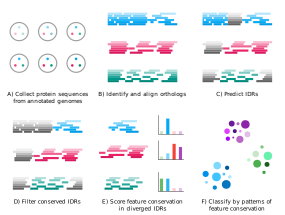
\includegraphics[width=\textwidth]{out/aims_overview.png}
\centering
\caption{\textbf{Graphical overview of aims.}
\textbf{(A)} The large open circles represent the genomes of different \textit{Drosophila} species, and the small, filled circles represent protein sequences in those genomes. Orthologs are colored with shades of the same hue. \textbf{(B-D)} Each horizontal line represents a sequence in panel A, and together each set of lines creates an alignment. The lines are broken where gaps are inserted to align equivalent segments. The grey segments denote regions of the alignment which are not part of subsequent analyses. \textbf{(E)} Each aligned IDR is scored on four features, where the strength of that feature is indicated by the height and color of its bar. \textbf{(F)} Scoring many IDRs on these features yields three distinct clusters.}
\label{fig:aims_overview}
\end{figure}

These comparisons, however, require the identification of IDRs with common ancestry that perform equivalent functions across many distinct organisms. Given the difficulties with identifying similar IDRs by their sequences, this may seem like a chicken and egg problem. Fortunately, IDRs are frequently associated with more conserved folded domains. Thus, identifying evolutionarily related proteins by their overall sequence signatures and aligning them will in turn identify the equivalent IDRs in those sequences. The first step of an evolutionary analysis of IDRs, then, is the identification of proteins with common ancestry, called orthologs. Since the first genomes were sequenced in the late 1990s, researchers have developed techniques for identifying and aligning orthologs~\cite{Fleischmann1995, Goffeau1996, CESC1998, Tatusov1997}. While these methods are generally effective, they are conducted by automated computational pipelines and prone to errors when processing the highly divergent sequences that characterize many IDRs. The evolutionary relationships between the genomes of closely related species generally make such mistakes easier to identify, and fortunately over the past five years advances in DNA sequencing technology have yielded dramatic increases in the number of sequenced genomes in the \textit{Drosophila} genus. However, because the existing methods for ortholog identification were designed for fewer or more distantly related genomes, they do not fully leverage such genomic redundancy to minimize errors. Thus, in the first chapter I develop a novel method for identifying orthologs which addresses this shortcoming and apply it to 33 \textit{Drosophila} genomes to generate a set of aligned orthologs (Fig.~\ref{fig:aims_overview}A-B). In the second chapter I then identify rapidly evolving IDRs in these alignments and analyse them with a variety of evolutionary models to detect patterns of conservation (Fig.~\ref{fig:aims_overview}C-F). Finally, in the third chapter I discuss several software tools and tutorials for fitting statistical models to data, which were created while pursuing the previous aims.


\chapter{Leveraging genomic redundancy to improve inference and alignment of orthologous proteins}
\graphicspath{{chapter1/figures/}}
\begin{abstract}
\noindent
Identifying protein sequences with common ancestry is a core task in bioinformatics and evolutionary biology. However, methods for inferring and aligning such sequences in annotated genomes have not kept pace with the increasing scale and complexity of the available data. Thus, in this work we implemented several improvements to the traditional methodology that more fully leverage the redundancy of closely related genomes and the organization of their annotations. Two highlights include the application of the more flexible \textit{k}-clique percolation algorithm for identifying clusters of orthologous proteins and the development of a novel technique for removing poorly supported regions of alignments with a phylogenetic HMM. In making the latter, we also wrote a fully documented Python package Homomorph that implements standard HMM algorithms and created a set of tutorials to promote its use by a wide audience. We applied the resulting pipeline to a set of 33 annotated \textit{Drosophila} genomes, generating 22,813 orthologous groups and 8,565 high-quality alignments.
\end{abstract}

\section*{Introduction}
Comparative genomics is a powerful tool for yielding insights into evolutionary relationships, molecular function, and the forces that drive gene, genome, and population evolution. These methods often rely on the identification of homologous sequences or homologs, that is sequences with common ancestry, since this ensures that differences between sequences reflect variations in evolution from a common point of divergence. However, many analyses impose the additional condition that the sequences have diverged through speciation events (orthology) rather than duplications (paralogy) or other mechanisms such as horizontal gene transfer~\cite{Fitch1970}. The underlying assumption is ``orthologs'' have conserved equivalent functions whereas ``paralogs'', by virtue of their redundancy, are more likely to diverge~\cite{Ohno1970, Nowak1997, Altenhoff2012, Pegueroles2013, Soria2014}.\footnote{For multiple sequences, orthology is usually defined relative to their most recent common ancestor. This technically includes sequences which split by duplication after this point (``in-paralogs''), but excludes sequences which split by duplication before (``out-paralogs'') \cite{Remm2001}. Many current orthology inference pipelines explicitly incorporate steps to detect in-paralogs. However, the resulting orthologs groups can easily be restricted to those without in-paralogs (``single copy orthologs'') for analyses where an assumption of conserved function is necessary.} This relationship between orthology and function is an essential component of modern biological research since it permits the transfer of annotations between biological systems using sequence similarity alone.

Given this importance, methods for inferring orthologous groups of proteins were developed shortly after the first genomes were sequenced in the late 1990s~\cite{Fleischmann1995, Goffeau1996, CESC1998}. One early and influential approach was to cluster triangles of hits resulting from homology searches between pairs of genomes~\cite{Tatusov1997}. Graph-based approaches have remained popular, and in the intervening years many other researchers have refined this method by implementing various pre- and post-processing steps. Despite these improvements, many databases and pipelines use the same triangle clustering algorithm or other methods which require relatively few hits between sequences to infer an orthologous group, \textit{e.g.} connected components or Markov clustering~\cite{Remm2001, Enright2002, Li2003, Jensen2007, Linard2011, Emms2015, Train2017, Cosentino2018}. However, the scale of biological sequence data has changed dramatically. For example, in the last decade, the number of annotated genomes available from NCBI has increased nearly 20-fold and currently exceeds 900 (Fig.~\ref{sfig:ncbi}). Though this figure is only a rough proxy of the total number of assemblies available, it will likely continue to grow rapidly in the coming years as many large-scale genome assembly efforts such as i5K, the Bird 10,000 Genomes Project, and the Vertebrate Genomes Project have already yielded results~\cite{Thomas2020, Feng2020, Rhie2021}. Thus, the dense taxonomic sampling made possible by these projects poses new challenges and opportunities for the standard methods of orthology inference and alignment, which implicitly assume fewer and more distantly related genomes or fail to fully leverage the redundancy and organization of their annotations.

In this work we therefore developed a computational pipeline that can robustly infer and align orthologous groups of proteins even when the genomes are highly redundant. Like many other orthology inference pipelines, our overall approach is based on clustering a graph of hits from homology searches. However, we modified many details to maximize the detection of highly diverged orthologs while also minimizing the impact of incomplete or incorrect annotations. Furthermore, since modern genome annotation pipelines frequently produce gene models and protein sequences in tandem, we implemented an additional clustering step to organize the resulting orthologous groups of proteins into gene-level units. However, most of our efforts were focused on the final step of aligning the orthologous sequences. Though genome annotation pipelines are often proficient at identifying the overall locus of genes, the accurate identification of exon boundaries and start codons when transcript evidence is limited remains an ongoing challenge~\cite{Frankish2015, Dunne2018}. Consequently, protein sequences derived from annotation pipelines can include non-homologous segments of significant length or exclude highly conserved segments. Such heterogeneity in the structure and length of the sequences in an orthologous group poses many challenges for their alignment and subsequent analysis. Thus, we implemented several novel quality control and data cleaning steps to correct mis-alignments and identify likely sequencing, assembly, or annotation errors.

To develop these methods, we chose a set of 33 assembled and annotated \textit{Drosophila} genomes, which includes all 12 species from the original \textit{Drosophila} 12 Genomes Consortium~\cite{D12GC2007}. However, the genomes of these 12 species have been re-sequenced since their first release, which has resulted in substantial improvements in their assemblies and annotations. Despite these developments and other several other recent genome assembly projects of species in the \textit{Drosophila} genus, there is not yet a collection of high-quality alignments of orthologous proteins that reflects these improvements in genome assembly and diversity~\cite{Miller2018, Kim2021}. Given the \textit{Drosophila} genus spans diverse habitats and over 50 million years of evolution but maintains a conserved life cycle and body plan, such a resource would facilitate a new generation of studies that illuminate the forces that drive protein evolution in unprecedented detail~\cite{Wiegmann2011, Obbard2012}.

\begin{figure}[h!]
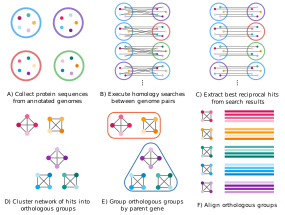
\includegraphics[width=\textwidth]{graphical_overview.png}
\centering
\caption{\textbf{Overview of homology inference pipeline.}
\textbf{(A-C)} The large, open circles represent the annotated genomes, and the small, filled circles represent the protein sequences associated with each annotation. Sequences that share homology are colored with shades of the same hue. \textbf{(D-F)} The small, filled circles and lines represent the same sequences and best hits from the previous steps.}
\label{fig:graphical_overview}
\end{figure}

\section*{Results}
\subsection*{Pipeline overview}
Our pipeline follows a similar overall approach to other graph-based methods of orthology inference. First, protein sequences from annotated genomes are collected (Fig.~\ref{fig:graphical_overview}A), and homology searches are then conducted between all query-target pairs of genomes (Fig.~\ref{fig:graphical_overview}B). The raw output from these homology searches is processed to yield best hits between pairs of sequences (Fig.~\ref{fig:graphical_overview}C). Next, the network of best hits is clustered into self-consistent orthologous groups (Fig.~\ref{fig:graphical_overview}D). Since genes can have multiplied associated isoforms, we then implemented a novel second clustering step where orthologous groups are grouped by their parent genes, which are represented by the two sets of clusters with warm and cool colors, respectively (Fig.~\ref{fig:graphical_overview}E). Finally, representative sequences in each orthologous group are aligned (Fig.~\ref{fig:graphical_overview}F). In the following sections, we discuss each of these and other steps which were omitted for clarity in greater detail.

\subsection*{Input genomes and pre-processing}
All annotated genomes in the genus \textit{Drosophila} available in April 2022 were downloaded from NCBI's RefSeq database. The assemblies annotated by the NCBI eukaryotic genome annotation pipeline have passed several quality checks and all have supporting transcript evidence, so the annotations are generally highly complete~\cite{Thibaud-Nissen2013}. The \textit{D. miranda} annotation was excluded due to its unusual karyotype~\cite{Dobzhansky1935}. Other annotations were excluded after preliminary clustering showed a deficiency in the number of orthologous groups containing those genomes, indicating their annotations were less complete (data not shown). The \textit{D. melanogaster} annotation was downloaded from FlyBase~\cite{Gramates2022}. In total, the input data consists of 33 genomes, which are listed in Table~\ref{stable:genomes}. Many genes have transcripts that differ only in their UTRs, and as a result there are many duplicate protein sequences in the annotations. Though not strictly necessary, we removed the duplicates in our pipeline, which greatly reduced the computational burden of later steps.

\subsection*{Extraction of best hits from BLAST output}
The protein sequences in each genome annotation were searched against each other in reciprocal pairs using BLAST, yielding a list of high-scoring segment pairs (HSPs) for each query-target pair~\cite{Camacho2009}. HSPs are local alignments, meaning they do not necessarily span the entire lengths of the query and target sequences. Consequently, the search algorithm may return multiple HSPs for each query-target pair if statistically significant regions of homology are separated by nonhomologous or poorly conserved regions. Though the most significant HSP is often used to represent all HSPs between a query-target pair, this approach can fail to rank the pairs by their overall significance if their alignments are broken into multiple HSPs. Furthermore, since query-target pairs were later filtered by the amount overlap between their sequences, it can also exclude pairs that pass the overlap threshold even if the most significant HSP alone does not. Thus, HSPs were merged into a single object called a hit. The best hits for each query were then taken as the highest-scoring hits that passed a minimum overlap criterion and were reciprocal between the query and target sequences.

\subsection*{Clustering in orthologous groups}
The best hits between sequences are naturally visualized as a graph where sequences are nodes and best hits are edges between nodes. Two connected components, sets of nodes joined by a sequence of edges, are shown (Fig.~\ref{fig:components}A,B). The sequences in the first (Fig.~\ref{fig:components}A) all contain C2H2 zinc fingers, whereas the sequences in the second (Fig.~\ref{fig:components}B) are members of the Par-1 family of serine/threonine protein kinases. In both components, some sets of nodes have a high density of edges, forming distinct clusters, whereas other nodes are only sparsely connected to their neighbors. To better understand the structure of these two components, we calculated the number of sequences, unique genes, and unique species in each. The first has 385, 346, and 33 sequences, genes, and species, respectively, and the second has 222, 33, and 33 sequences, genes, and species, respectively. We then plotted the relationship between the number sequences and unique genes across all components to see if this pattern holds true generally (Fig.~\ref{fig:components}C). Two distinct trendlines are apparent. The first increases linearly with the number of sequences with a slope of one, indicating each sequence is generally associated with a unique gene. The second is constant with an intercept of 33, indicating the number of unique genes quickly saturates at the total number of genomes. Thus, there are generally two classes of components. The first is composed of many distinct genes, whereas the second is composed of many different isoforms of a single group of genes.

The diffuse networks observed in the first component class are likely the result of a combination of factors, including rapid evolution, gene duplication, and annotation errors. Regardless of their origin, these hits are not strong candidates for comparative analyses since an orthology relationship is supported by relatively few genome pairs. Instead, likely orthologs should consistently identify each other as best reciprocal hits across many genome pairs. The same is true of the hits in the second component class. Although the genes as a unit form a single orthologous group, sequences with few hits are likely non-conserved or tissue-specific isoforms. Thus, orthologous groups can be operationally defined as self-consistent clusters in the hit graph. However, sequence divergence or assembly and annotation errors may prevent a best reciprocal hit between orthologous sequences across all genome pairs. In fact, although the most common number of reciprocal hits is 32, one fewer than the total number of genomes, many sequences have fewer (Fig.~\ref{fig:components}D). Thus, the clustering method should require a high degree of self-consistency without demanding complete consensus.

\begin{figure}[h!]
\includegraphics[width=\textwidth]{components/out/0017-005F.png}
\centering
\caption{\textbf{Selected connected components of hit graph and summary statistics.}
\textbf{(A-B)} Two distinct connected components of the hit graph. Edges are colored by the value of their bit score. \textbf{(C)} Hexbin plot of the number of sequences and the number of unique genes in each component. \textbf{(D)} Histogram of number edges associated with each sequence, \textit{i.e.} the degree of each node. Only the lower 99th percentile of the distribution is shown.}
\label{fig:components}
\end{figure}

The identification of sets of densely connected nodes in graphs is known as community detection in network analysis. While many community detection algorithms are available, only some are commonly used in the context of orthology inference. One early method that remains popular is building clusters progressively by identifying nodes that form a triangle with at least two other nodes in the cluster~\cite{Tatusov1997, Jensen2007}. Other approaches include the MCL algorithm, which clusters graphs by similating stochastic flow, and connected components or other single-linkage criteria~\cite{Remm2001, Enright2002, Li2003, Emms2015, Train2017, Cosentino2018}. While these methods are robust when clustering hit graphs derived from smaller or more diverse sets of genomes, they are not suitable for the large number of closely related genomes in this work since they require relatively few edges to define a cluster. For example, the MCL algorithm and connected components method assign a node to a cluster as long as it has a single edge, and triangle clustering only requires two edges to two adjacent nodes.

However, connected components and triangle clustering are special cases of the more general \textit{k}-clique percolation algorithm where \textit{k} equals two and three, respectively. The clique percolation algorithm detects clusters by first identifying cliques, sets of nodes which are fully connected, of a specified size \textit{k} in the graph (Fig.~\ref{fig:percolation}A). Clusters are then taken as the connected components of an overlap graph where an edge exists between two cliques if they share \textit{k}-1 nodes in common. An intuitive way to visualize this algorithm is by ``rolling'' a clique of some size \textit{k} over the graph (Fig.~\ref{fig:percolation}B). More specifically, a cluster is initiated when a set of nodes which form a \textit{k}-clique is identified. The cluster expands by shifting the \textit{k}-clique to an adjacent \textit{k}-clique that shares \textit{k}-1 nodes in common with the current \textit{k}-clique. A cluster stops expanding when there are no adjacent \textit{k}-cliques, and the algorithm terminates when there are no \textit{k}-cliques which are not part of a cluster. The strength of this algorithm is its ability to exclude sparsely connected nodes from clusters with an easily tunable parameter \textit{k}. Higher values of \textit{k} require greater overlap between a candidate node and those already in the cluster and therefore produce tighter clusters at the cost of excluding more speculative orthology relationships (Fig.~\ref{fig:percolation}C). We set \textit{k} to four as compromise between these concerns, yielding 22,813 orthologous groups, a plurality of which contained all 33 species (Fig.~\ref{sfig:clusters}).

\begin{figure}[h!]
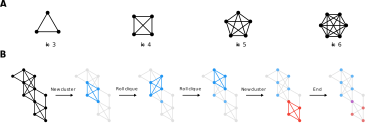
\includegraphics[width=\textwidth]{percolation/percolation.png}
\includegraphics[width=\textwidth]{percolation/out/005F.png}
\centering
\caption{\textbf{Clique percolation algorithm.}
\textbf{(A)} Cliques for \textit{k} equal to three, four, five, and six. \textit{k} equal to one and two correspond to a single node and two nodes joined by an edge, respectively. \textbf{(B)} Illustration of clique percolation algorithm where \textit{k = 4}. \textbf{(C)} A single component clustered by clique percolation with varying values of \textit{k}. Nodes are colored according to their cluster. If a node belongs to multiple clusters, it uses a blend of those colors.}
\label{fig:percolation}
\end{figure}

\subsection*{Addition of paralogs to orthologous groups}
A weakness of the best reciprocal hits criterion is its exclusion of recently diverged paralogs. Since only the highest scoring hits for each query are included in the graph, a paralog without a corresponding duplicate in the target genome is ignored if it is marginally more diverged than the other copy. This is corrected by adding likely paralogs to the orthologous groups. Briefly, the protein sequences in each genome were searched against themselves. If the bit score for an intra-genome hit exceeded the bit score of any inter-genome hits for the same query, the two sequences were identified as a paralogous pair. Orthologous groups were then supplemented with paralogs by adding the paired sequences for each of the original members of the orthologous group. Most orthologous groups contain no paralogs, and those that do generally have few relative to the original number of sequences in the group (Fig.~\ref{sfig:paralogs}).

\subsection*{Grouping orthologous groups by gene}
As genes can have several annotated isoforms, each gene can be associated with several orthologous groups. However, the orthologous groups are not organized into gene-level units since they were clustered using sequence similarity only. A graph-based approach was therefore used to group orthologous groups with similar sets of parent genes. First, a gene overlap graph was constructed by defining an edge between orthologous groups if the intersection of their associated sets of parent genes is at least 50\% of the smaller of the two. Gene groups were then taken as the connected components of the resulting graph, yielding 14,909 groups. This is commensurate with the roughly 15,000 genes in each genome, which suggests this approach has successfully clustered orthologous groups derived from a common set of parent genes.

\subsection*{Initial alignment and selection of representative sequences}
Since the NCBI annotation pipeline incorporates transcriptome data from a variety of sources, its inputs are heterogeneous in sequencing depth, developmental stage, and tissue of origin across different genomes. As a result, some genomes are annotated with different or multiple splice isoforms of a given orthologous gene, which can create complex networks in the resulting hit graph. For example, if the genomes are variably annotated with one or both of two distinct isoforms, the resulting graph may contain two clusters connected by a ``bridge'' formed by the genomes which contain only one of the isoforms. If the nodes bridging the two clusters form cliques with themselves and the clusters, the clique percolation algorithm will merge all the nodes into a single orthologous group where some genes have multiple associated sequences. However, these additional sequences can complicate downstream comparative analyses that may not easily generalize to genes with multiple associated sequences. Thus, in our pipeline a single representative was chosen for each gene using an alignment-based strategy detailed in the methods section. Briefly, a statistical profile was created from an alignment of the sequences in each orthologous group, and the representative for each gene was chosen as the sequence which best matched this profile.

\subsection*{Selection of single copy orthologous groups}
The criteria for selecting orthologous groups for further analyses depends on the biological question under investigation. For example, studies of gene duplication will focus on orthologous groups with paralogs in some lineages but not in others. In contrast, analyses which assume functional conservation should restrict the orthologous groups to single copy orthologs since paralogs more frequently undergo functional divergence~\cite{Altenhoff2012, Pegueroles2013, Soria2014}. A simple method for identifying such groups is requiring each species to have exactly one associated gene. However, since the probability of at least one missing gene annotation approaches one as the total number of genomes increases, this is too restrictive and fails to leverage the redundancy of closely related genomes. Instead, a set of phylogenetic diversity criteria detailed in Table~\ref{stable:diversity_criteria} were applied to ensure the major lineages were represented in downstream analyses. Furthermore, genome-wide analyses should select one orthologous group per each of the previously identified gene groups as to not bias the results towards genes with many distinct groups of isoforms. In summary, orthologous groups failing the phylogenetic diversity criteria were first removed, and the representative for each gene group was chosen as the highest scoring orthologous group when ranked by the number species and the sum of the bit scores associated with each edge. This significantly reduced the number of orthologous groups from 22,813 to 8,566.

\subsection*{Alignment refinement}
Though the pipeline’s quality control measures ensure a high degree of overall sequence identity between members of an orthologous group, some sequences contain long ``poorly supported'' segments which have no homology to most or any other sequences in the alignment. Since most common multiple sequence alignment algorithms assume the sequences are largely homologous, these segments are sometimes ``over-aligned'' by forcing them into alignment where chance sequence similarities occur. Typically, these segments remain contiguous, so the alignments alternate between short runs of columns with few or no gaps and large gap-rich regions (Fig.~\ref{fig:realignment}A-B, left). More rarely, when long poorly supported segments are adjacent to a long gap in the same sequence, the two are interlaced, yielding long gaps interrupted by short segments of spurious alignment (Fig.~\ref{fig:realignment}C, left).

The aligner MAFFT has a mode for addressing over-alignment with a parameter, \textit{a\textsubscript{max}}, that adjusts the strength of the correction~\cite{Katoh2013, Katoh2016}. \textit{a\textsubscript{max}} varies between 0 and 1, with higher values yielding a stronger correction. While values above 0.8 completely eliminate over-alignment and successfully align highly conserved regions, the alignment as a whole is severely degraded, as even homologous sequences with a small amount of divergence are separated by gaps. Thus, in our pipeline orthologous groups were aligned in two stages. In the first, the sequences were aligned with a strong correction of 0.7. Highly conserved regions were identified, which divided the alignment into a complementary set of diverged regions. The sequences in each of these regions were then extracted and aligned separately with a more conservative value for \textit{a\textsubscript{max}} of 0.4. The resulting ``sub-alignments'' were ``stitched'' back into their positions in the original alignment. By defining highly conserved ``anchor'' regions, this approach largely prevents the alignment of chance sequence similarities in long poorly supported segments (Fig.~\ref{fig:realignment}, right).

\begin{figure}[h!]
\includegraphics[width=\textwidth]{realignment/out/merged.png}
\centering
\caption{\textbf{Alignment with long poorly supported segments.}
The alignments of representative sequences in orthologous groups 0167 \textbf{(A)}, 2770 \textbf{(B)}, and 23D9 \textbf{(C)} before and after refinement.}
\label{fig:realignment}
\end{figure}

\subsection*{Alignment curation}
Although the refinement process corrects most cases of over-alignment, the alignment may still contain regions whose aligned segments have poor or inconsistent support. For example, long poorly supported segments in internal regions were not removed from the alignment since they are bounded by at least one consensus column to the left and right. Additionally, some regions have a significant fraction of sequences with strongly supported segments, but the observed gap pattern is discordant with the expected phylogenetic relationships. Since they are present in so few sequences, the former segments are likely artifactual, resulting from errors during assembly or annotation. (Biological explanations such as alternative splice sites, frameshift mutations, or transposition events are also possible, however.) In contrast, the high sequence identity and clear boundaries of the segments in the latter regions suggest they are conserved but skipped exons. Given the heterogeneous sourcing of the transcript evidence, these sequences containing these segments are likely splice isoforms specific to certain tissues or developmental stage.

% To investigate these hypotheses, the genome sequences and supporting transcript evidence for several segments and regions were examined in detail: 0254, 26CF, 202C, 188E, 2E9F, 34B7, 0C31.

Since the segments in these regions are likely the result of incorrect or incomplete annotations rather than meaningful biological variation, maintaining them in the alignments would propagate spurious homologies to subsequent analyses. This is a common issue in alignments generated by automated pipelines, so downstream analyses often focus on the strongly supported regions by removing or ``trimming'' columns below some threshold number of gaps or sequence identity~\cite{Castresana2000, CapellaGutierrez2009}. This approach, however, is inadequate if the taxonomic sampling is dense, as a single indel event along a lineage containing many species can increase the number of gaps above the threshold. Moreover, as this method does not incorporate any spatial information, it can rapidly alternate between trimming and preserving columns. Thus, it can severely disrupt any analyses which are sensitive to the spatial organization of an alignment.

Phylogenetic HMMs (phylo-HMMs) are statistical models that incorporate phylogenetic and spatial information to calculate the probability that each observation in a sequence was generated by one of several ``hidden states''~\cite{Felsenstein1996}. Since they can evaluate both the probability of a gap pattern in a column given the known phylogenetic relationships and the local context, a phylo-HMM was used to segment the alignment into contiguous regions with different patterns of gaps. A fully specified phylo-HMM requires a fixed number of hidden states and a probability distribution for each. Thus, we identified four distinct types of regions in the alignments, roughly corresponding to highly conserved regions with few to no gaps, diverged regions, regions with a stable gap pattern discordant with the expected phylogenetic relationships, and regions with poorly supported segments. For simplicity, however, we refer to the states that generate each type of region as 1A, 1B, 2, and 3, respectively. To model probability distributions for each state, we first conceptualized the observed alignments as the superposition of two distinct processes (Fig.~\ref{fig:hmm}A, left). The first is a phylogenetic process which evolves and splits a single ancestral sequence over time according to a tree. The second is the annotation process which can erroneously exclude or include segments from a sequence. The result is an alignment of annotated sequences which contains evolutionary information obscured by ``noise'' from the annotation process, shown here by the exclusion of three N-terminal residues in the fourth annotated sequence. To simplify modeling this behavior with an HMM, we coded the sequences into binary symbols. The distributions for each state then consisted of two components derived from the encoded sequences (Fig.~\ref{fig:hmm}A, right). The first component models the gap pattern with a Markov process. This Markov process is in turn composed of two subprocesses where the first is a phylogenetic process, and the second is a jump process. These subprocess roughly correspond to changes caused by evolution and annotation, respectively. Because this first component did not fully capture the propensity for the gap patterns to remain constant, we included a second component that models the ``gap stickiness'' as a beta-binomial random variable by counting the number of symbols that remain constant between columns. Each component is associated with a set of parameters, and the unique parameters for each state yield its characteristic gap pattern and gap stickiness.

After the model was trained on manually labeled examples, it was used to assign a label to the columns in each alignment. Columns assigned to states 1A and 1B are the regions of interest for downstream analyses since the gaps generally follow the expected pattern given the phylogenetic tree. In contrast, columns assigned to states 2 and 3 largely corresponded to the long poorly supported segments and phylogenetically discordant regions discussed previously and were therefore removed from the alignments. In the example decoded alignment shown, the decoded states closely follow the expected patterns (Fig.~\ref{fig:hmm}B). Overall, fewer than 10\% of alignments were trimmed of any regions. However, when regions were trimmed, they were largely inferred as state 3, meaning the removed regions are generally long poorly supported segments that are aligned to few if any other sequences (Fig.~\ref{sfig:insertion_trim}).

% TODO: Update text for new figure

\begin{figure}[h!]
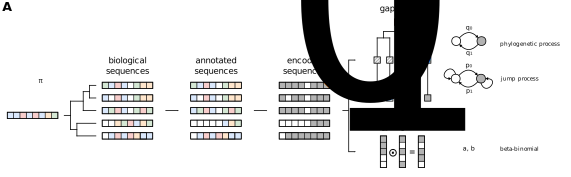
\includegraphics[width=\textwidth]{hmm/hmm_architecture.png}
\includegraphics[width=\textwidth]{hmm/out/2252.png}
\centering
\caption{\textbf{HMM emission architecture and a decoded alignment.}
\textbf{(A)} Schematic of theoretical alignment generating process and corresponding probabilistic components in HMM. White and colored boxes indicate gap and non-gap symbols in the biological sequences, respectively. White and grey boxes indicate gap and non-gap symbols in the encoded sequences, respectively. c\textsubscript{0} and c\textsubscript{1} indicate the first and second columns in the alignment, respectively. The parameters associated with each component are shown to the right. \textbf{(B)} The alignment of the representative sequences in orthologous group 2252 decoded using the trained HMM.}
\label{fig:hmm}
\end{figure}

Though the phylo-HMM removed phylogenetically incongruent ``insertions,'' some sequences still contained extensive segments of uninterrupted gaps. These segments are easily identified in regions which are otherwise highly conserved, so they are also likely the result of incorrect or incomplete annotations. Unfortunately, they can also span more diverged regions, which complicates a simple rule- or threshold-based approach for identifying them. Thus, another phylo-HMM was trained to label each position in a sequence as generated by either a ``missing'' or ``not missing'' state. In this case, however, the aligned sequences were processed individually and not as aligned columns. As the previous phylo-HMM already ensured each column has sufficient support, these labels can instead be used to exclude sequences from downstream analyses depending on the amount of tolerated overlap with the regions of interest.

\subsection*{Inference of species trees}
Many phylogenetic methods require a species tree to inform the evolutionary relationships between sequences. In fact, the phylo-HMMs discussed previously used a species tree as an input, though we omitted this detail for clarity of exposition. Therefore, to support the curation step and other downstream analyses, we sought to infer phylogenetic trees from the aligned sequences. However, since the roots of phylogenetic trees are not identifiable with commonly used time-reversible substitution models, we repeated the orthology inference pipeline with the outgroup species \textit{Scaptodrosophila lebanonensis}. Afterwards, we inferred phylogenetic trees using the LG model of amino acid substitution from 100 meta-alignments sampled from alignments of single copy orthologous groups. We then combined them into a single consensus tree (Fig.~\ref{fig:trees}A). To provide a similar tree for the analysis of non-coding regions, we inferred phylogenetic trees using the GTR model of nucleotide substitution from 100 meta-alignments sampled from nucleotide alignments which were ``reverse translated'' from the protein alignments and their corresponding coding sequences (\ref{fig:trees}B). Both trees have an identical topology, which is consistent with other published phylogenies~\cite{D12GC2007, DaLage2007}.

\begin{figure}[h!]
\includegraphics[width=\textwidth]{trees/out/trees1.png}
\centering
\caption{\textbf{Phylogenetic tree of species.}
\textbf{(A)} Consensus tree from LG model fit to meta-alignments directly sampled from the original protein alignments. \textbf{(B)} Consensus tree from GTR model fit to meta-alignments sampled from ``reverse translated'' nucleotide alignments. Values at nodes are bootstrap percentages.}
\label{fig:trees}
\end{figure}

\section*{Discussion}
The orthologous groups and alignments yielded by this pipeline are a valuable resource for comparative studies of gene birth/death processes and protein evolution at the level of both entire proteomes and specific gene families in the \textit{Drosophila} genus. To assist these efforts, the final alignments after curation and the labels from the ``missing'' phylo-HMM are provided as supplemental data. Although this work focused on single copy orthologs, other studies may require different subsets of orthologous groups that demand other pre-processing and alignment strategies. Therefore, we have included the orthologous groups and the initial alignments with and without non-representative sequences in the supplemental data as well. While we anticipate these resources will remain relevant in the near term, the trends that permitted this work to substantially improve on previous efforts will render them obsolete in the coming years as more \textit{Drosophila} genomes are assembled and annotated. However, an authoritative and lasting set of orthologous groups and alignments is not the primary goal of this work. Instead, it serves as a case study in how dense taxonomic sampling and modern genome assembly and annotation pipelines present new opportunities and challenges to the traditional techniques for identifying and aligning orthologous groups.

For example, despite many additional pre-processing steps and other tweaks introduced by later authors, the basic framework of orthology inference by clustering the hit graph has remained largely unchanged in the past twenty years~\cite{Tatusov1997, Remm2001, Li2003, Jensen2007, Linard2011, Emms2015, Train2017, Cosentino2018}. This longevity is a testament to the robustness of the underlying idea that orthologous proteins should consistently identify each other as the most similar pairs between their genomes. Even as the number of genomes and their taxonomic density has increased dramatically, many orthology inference pipelines continue to use algorithms which were originally applied to sets of far fewer and more distantly related genomes. This mismatch in scale increases the chance of propagating annotation errors since only a small number of edges are needed to create or merge clusters. Thus, we instead applied a generalization of the triangle and connected components clustering methods called \textit{k}-clique percolation where \textit{k} is a tunable parameter that influences the tightness of a cluster. The optimal value of \textit{k} for a given set of genomes is unclear and likely depends on the desired trade-off between sensitivity and specificity. Furthermore, \textit{k} is not necessarily a global parameter and can instead depend on the properties of each connected component. For example, one possibility is to take an entire component as an orthologous group if its number of unique genes and unique species are equal since all the sequences are isoforms of a single set of genes. This would effectively set \text{k} equal to one for this component. Another approach is to make \textit{k} an decreasing function of the density of edges, so sparser graphs are clustered more permissively. However, percolation theory or simulations may yield additional insights.

Another challenge is the annotation of multiple isoforms for a single gene. Though prior pipelines have generally selected the longest isoform as the representative before conducting the orthology searches, if the sequences do not share a common intron-exon structure this approach can introduce artifacts or other issues during alignment. Instead, as protein sequences are increasingly derived from or linked to genomic sequences, we sought to incorporate the full annotations into the orthology inference pipeline. This, however, created two additional complications. First, a single gene could have several associated orthologous groups if its isoforms belonged to different clusters. Second, a single orthologous group could have several isoforms of a single gene if its isoforms were clustered together. In both cases, the presence of multiple sequences for a single gene creates ambiguities over which is the ``primary'' isoform. Since the first occurs at the level of orthologous groups, the orthologous groups were first grouped by the similarity of their parent genes using a graph-based strategy. Afterwards, a single representative is easily chosen as the group with the largest number of distinct species, though other criteria are possible. Since the second occurs within an orthologous group, the sequences were first aligned, and a representative for each gene was chosen as the sequence which was most concordant with this initial alignment.

The second major innovation in this work is its method for the refinement and trimming of alignments. Since sequences produced from automated annotation pipelines can contain long segments which are not homologous to most or any other sequences in their respective orthologous groups, their alignments may contain over-aligned or poorly supported regions which can introduce artifacts into downstream analyses. Thus, in refinement over-alignment is avoided by aligning the sequences in two stages. In the first highly conserved regions are aligned using a strong correction for over-alignment, and in the second more diverged regions are aligned with a weaker correction. This process usually prevents errors caused by long poorly supported segments without degrading the quality of the alignment. In trimming, a phylo-HMM is used to remove regions which are poorly supported by the phylogenetic consensus.

While the combination of these two steps yielded high-quality alignments that are suitable for further analyses, they are an \textit{ad hoc} fix for underlying issues with the gene models and alignment algorithms. The most principled solution is to optimize or supplement the gene models using the initial alignments generated by the orthology inference pipeline, which is possible with tools such as OMGene or OrthoFiller~\cite{Dunne2018, Dunne2017}. However, if preserving the original annotations is desired or necessary, the remaining possibility is to correct the alignments as we have done here. In fact, the errors we sought to address broadly stem from shortcomings of current alignment algorithms rather than errors in the sequences themselves. Though the scoring functions of modern multiple sequence alignment algorithms are complex, they are generally derived from models that penalize gaps with a linear or affine cost. As a result, they often interlace gaps with short, aligned segments rather than a single long gap. However, when the sequences are different isoforms of a single gene, their alignment will necessarily contain contiguous exon sized gaps. The same is true when aligning isoforms of diverged orthologs, though the relationship between their exons may be complex.

The most popular aligners for protein sequences (Clustal Omega, MAFFT, MUSCLE, T-Coffee) do not include splice sites in their alignments, which makes them prone to aligning non-homologous exons~\cite{Sievers2017, Katoh2013, Edgar2004, Notredame2000}. Current algorithms can easily be extended to incorporate splice sites by coding them as a new symbol and preventing alignment between splice sites and amino acids, which was recently implemented in the aligner, \textit{Mirage}~\cite{Nord2018}. The biggest challenge in practice, however, is mapping a protein sequence to its genomic sequence to identify splice sites in the protein sequence. Although this information can in principle be derived from the GTF annotation files produced by the NCBI pipeline, annotating the splice junctions in the protein sequences themselves would facilitate splice-sensitive alignment.

These improvements would enhance rather than replace the phylo-HMM trimming method developed in this work. The model could easily be extended to include a state that outputs a splice symbol before transitioning to one of the states in the current architecture. This intermediate state would increase the accuracy of state inference since a splice symbol followed by a phylogenetically discordant gap pattern would strongly signal a state 2 region. The association between state 2 and skipped exons can be made explicit by requiring that transitions to and from state 2 first proceed through the splice state. This of course depends on proper labeling of the training data, which would be trivial since the boundaries between exons would be marked by splice site symbols rather than inferred from gap patterns. Unfortunately, this would not allow the phylo-HMM to label extended exon boundaries as state 2 since they would not be bounded by splice symbols to the left and right. Accordingly, the phylo-HMM would need to permit transitions between state 3 and any other state to accommodate more complex splice variants and other annotation errors. Thus, this extended phylo-HMM would combine the strengths of splice-sensitive alignment with the more heuristic approach used here. Since state 2 inferences would necessarily correspond to skipped exons, they would be suitable for analyses of this form of alternative splicing. Though state 3 inferences would not directly correspond to specific biological process, they still have value as spatially and phylogenetically aware labels for trimming poorly supported segments from alignments.

The phylo-HMM could be further enhanced by expanding its emission distribution to include more symbols in the amino acid alphabet. This would allow it to better model observed substitution patterns between specific symbols, for example the high rate of exchange between gaps and glutamine residues caused by polyglutamine tracts. The transitions between amino acids could be parametrized with a published matrix such as LG~\cite{Le2008}, but the transitions between amino acids and gaps would be inferred from labeled data. It is unclear if the resulting gain in accuracy would justify the increased computational burden, however.

Though there are benchmarks available for optimizing and comparing methods of orthology inference, the metrics are calculated over a set of reference genomes which are sparsely sampled over a broad taxonomic range, so it is unclear if they are informative for method designed to yield robust inferences when the genomes are highly related~\cite{Nevers2022}. Furthermore, the heterogeneity of genome architectures and annotations may require quality assurance methods tailored to each set of genomes. Thus, there is likely no one-size-fits-all approach to orthology inference, and with many other standalone programs available for more standard use cases (Hieranoid, OMA standalone, OrthoFinder, OrthoInspector, Orthologer), we have chosen not to package the code into an end-to-end pipeline~\cite{Kaduk2017, Altenhoff2019, Emms2019, Linard2014, Zdobnov2020}. Instead, we have devoted considerable attention to organizing and documenting the code to make it accessible to a newcomer and thereby facilitate the adaptation of specific steps to similar projects as needed.

In contrast, though many HMM packages are available for the Python programming language, we found none were satisfactorily documented or contained tutorials to introduce HMMs and their APIs to a wide audience. We therefore refactored this code into a package available on PyPI and GitHub called Homomorph. The package itself only implements standard HMM algorithms, but the GitHub repository includes tutorials that introduce the API and implement training routines. Similar tutorials for machine learning libraries such as TensorFlow have undoubtedly fueled the application of neural networks across diverse fields, but HMMs are also powerful models that can be more appropriate when the data obey certain statistical or structural constraints. Thus, we hope this package and its accompanying tutorials will serve as an on-ramp to HMMs and spur their greater adoption by non-specialists.

Though databases of orthologous groups such as COGs, Ensembl Compara, EggNOG, OMA, OrthoDB, OrthoInspector, and OrthoMCL will continue to be useful for comparative studies across broad taxonomic ranges, the increasing speed at which high-quality genome assemblies and annotations are produced means no single database can encompass the most complete data~\cite{Galperin2020, Herrero2016, HuertaCepas2018, Altenhoff2020, Zdobnov2020, Nevers2018, Chen2006}. Furthermore, since many early comparative genomics studies spanned diverse branches of the tree of life, future research will likely prioritize taxonomic depth over breadth. Thus, custom sets of orthologous groups will grow more and not less common. Despite the challenges these developments pose, they also present new opportunities to bridge the gap between mutational and macroevolutionary processes.

\section*{Materials and methods}
\subsection*{Sequence de-duplication and BLAST search parameters}
The protein sequences for each annotation were de-duplicated by removing any sequences which had already appeared in association with the same gene. Thus, the first accession associated with a sequence and gene pair is the sequence’s representative accession for the gene. BLAST+ 2.13.0 was used for the sequence similarity searches~\cite{Camacho2009}. An E-value cutoff of 1 was used for the initial searches. However, this cutoff was lowered to 1E-10 during processing of the BLAST output.

\subsection*{Extraction of HSPs from BLAST output}
To reduce the computational burden of merging HSPs into hits, the BLAST output was filtered to extract HSPs associated with the highest-scoring gene. The HSPs were first grouped by target protein, and the resulting groups were sorted in descending order by the bit score of their highest-scoring HSP. Iterating over the groups, all the HSPs in a group were passed to the next step until the parent gene of the group was not the parent gene of the highest ranked group. This method collects all candidate HSPs for a target gene if the highest-scoring HSP within a group exceeds the highest-scoring HSP of the next best gene. This is in some senses an extension of the best hit criterion where hits are considered at the level of genes rather than proteins. If multiple genes tied for the highest-scoring HSP, the iteration stopped when the parent gene of the current group matched none of these highest-scoring genes.

\subsection*{Merging of HSPs into hits}
HSPs were merged in two stages where the first combined non-overlapping HSPs, and the second combined the remaining HSPs. In the first stage, proceeding from highest to lowest bit score, HSPs were marked as ``disjoint'' if they do not overlap with any other HSP previously marked as disjoint. Although this greedy strategy does not necessarily yield the highest-scoring set of disjoint HSPs, it prioritized higher scoring HSPs. In the second stage, all disjoint HSPs were marked as ``compatible,'' and proceeding from highest to lowest bit score the remaining HSPs were marked as compatible if the overlap with any other compatible HSP was no more than 50\% of the length of either. The best hit for each query was chosen as the hit with the highest sum of bit scores from disjoint HSPs. The best hits were then filtered by overlap and reciprocity criteria. The overlap criterion was applied first and requires that 50\% of residues in the query are aligned in compatible HSPs. This excludes false positives from conserved domains embedded in larger non-homologous proteins by ensuring the hits span a sufficient fraction of the query and target sequences. The reciprocity criterion requires each query-target pair has a corresponding hit where the roles are reversed, which ensures there is no ambiguity in which target is the best match for the query.

\subsection*{Clustering by \textit{k}-clique percolation}
\textit{k}-clique percolation was implemented in two steps. In the first, maximal cliques were identified. In the second, a percolation graph is constructed by defining edges between cliques if they have \textit{k}-1 nodes in common. Clusters are the connected components of this second graph. The first step uses the NetworkX implementation of a maximal clique algorithm. The second step uses a modification of the NetworkX implementation of the \textit{k}-clique community algorithm. The NetworkX implementation exhaustively finds all edges in the percolation graph. Since joining a \textit{k}-clique community only requires that a clique has a single edge connecting it to that a community, this approach is needlessly expensive for large graphs. The custom implementation instead uses a progressive approach where each clique is checked against a list of known communities, merging communities as necessary in each step.

The hit graph is sparse, so these algorithms are efficient when applied to its individual connected components. However, some components have a structure with many maximal cliques, which dramatically slows the first or second step of the clique percolation algorithm. Thus, if either step exceeded 90 s, the process timed out, and the simpler \textit{k}-core algorithm was used instead. Out of over 10,000 connected components, only seven timed out, and many of those contained highly dense clusters of histone sequences.

\subsection*{Addition of paralogs to orthologous groups}
The protein sequences for each annotation were searched against themselves with the same settings as for the inter-genome searches. The resulting output was processed identically except the HSPs were not filtered using the best gene criterion. Thus, all HSPs for each query were merged into hits. The best hit for each query and target gene was then chosen as the hit with the highest sum of bit scores from disjoint HSPs. (Grouping by target gene ensured only the highest-scoring isoform was selected.) Query-target pairs whose hits which exceeded the maximum bit score for all inter-genome hits associated with that query and passed the overlap and reciprocity filters were designated as paralogous pairs. The orthologous groups were supplemented with paralogs by adding the paired sequences for each of the original members of the orthologous group.

\subsection*{Initial alignment and selection of representative sequences}
The sequences in each orthologous group were aligned using MAFFT 7.490 with the following settings: -{}-globalpair -{}-maxiterate 1000 -{}-thread 1 -{}-anysymbol -{}-allowshift -{}-leavegappyregion -{}-unalignlevel 0.4~\cite{Katoh2013}. Representative sequences for each gene were then selected by maximum likelihood according to binary profiles constructed from these alignments. First each sequence was coded into gap and non-gap symbols. The sequences were then grouped by gene, and for each group and position if at least one sequence was aligned in the group, the group contributed one count for the non-gap symbol to the profile at that position. Otherwise, the group contributed a count for the gap symbol at that position. To account for the phylogenetic dependencies between sequences, the counts were weighted according to a Gaussian process over the GTR2 consensus tree described in the section on inferring species trees~\cite{Altschul1989}. If a species had multiple genes in the orthologous group, the species weight was divided evenly among them. Each coded sequence was then scored according to this profile, and the maximum likelihood sequence for each gene was selected as its representative. By assigning a non-gap count to groups and positions where at least one sequence is aligned, the profile incentivizes the selection of sequences contain the fewest gaps and match the consensus alignment. Unfortunately, this scheme can cause a sequence to score negative infinity if it has a gap at a position where every group has at least one aligned sequence, so the profile was initialized with a pseudocount of 0.005 for the gap and non-gap symbols at each position.

\subsection*{Alignment refinement}
The representative sequences in the single copy orthologous groups were aligned with the same settings as described in the previous section except \textit{a\textsubscript{max}} was set to 0.7. A binary profile was created from the alignment using Gaussian process sequence weighting as described in the section on selecting representative sequences. (Because the orthologous groups were single copy and contained only representative sequences, each sequence received the full weight associated with its species.) The binary profile was then converted into a binary mask by identifying where the weighted fraction of non-gap symbols exceeded 0.5. The binary mask was closed with a structuring element of size three, and highly conserved regions were identified as the contiguous intervals of this closed mask with a minimum length of 10. Diverged regions were taken as the complement of the highly conserved regions. For each diverged region, the corresponding segments of the sequences in the initial alignment were extracted and aligned with \textit{a\textsubscript{max}} set to 0.4. The resulting sub-alignments were then stitched into the initial alignment.

\subsection*{Alignment curation}
The alignments were coded into gap and non-gap symbols to simplify the emission distributions. The ``insertion'' phylo-HMM was composed of the four hidden states described in the main text. The emission distributions for each consisted of two components which modeled the gap pattern and the propensity for those patterns to remain constant (``gap stickiness''), respectively. The first component was a two-state Markov process which was in turn composed of two subprocess. The first was a phylogenetic process on the on the GTR2 consensus tree described in the section on inferring species trees, and the second was jump process at the tips. The second component was a beta-Bernoulli distribution on the number of symbols which were constant between subsequent columns. The ``missing data'' phylo-HMM was composed of two hidden states which were both parameterized with the same two-state, two component Markov process as the insertion phylo-HMM. However, the emission probabilities were calculated as the posterior probability of the observed symbol given the data rather than the probability of the data. Only the alignments of the single copy orthologous groups were curated, so each tip in the species tree would correspond to a single sequence in the alignment.

All HMM algorithms were implemented with custom code which is available as the package Homomorph on PyPI. The insertion phylo-HMM was trained on 39,298 manually labeled columns in 11 alignments, and the deletion phylo-HMM was trained on 58,655 manually labeled positions in 20 sequences in 9 unique alignments (Fig.~\ref{sfig:insertion_training}, Fig.~\ref{sfig:missing_training}). Because maximum-likelihood estimation of the model parameters yielded posterior decoding curves which toggled between hidden states too rapidly, the models were instead trained discriminatively~\cite{Krogh1999}. The difference, briefly, is maximum-likelihood estimation finds the parameters that best reproduce the observed distributions whereas discriminative training finds the parameters that minimize prediction error. Discriminatively trained models typically perform better in practice since real-world data are rarely fully described by the distribution specified by the model.

The posterior distributions over states were calculated for each alignment using the trained insertion phylo-HMM. States 2 and 3 have distinct characteristics which require different trimming strategies, so regions with a high probability of state 3 were handled first. Because the posterior probability of a state can change rapidly or gradually depending on the local context, a simple cutoff would not necessarily define the boundaries as the columns where the gap pattern changes most abruptly. Instead, a high cutoff of 0.95 was used to define a ``seed'' region. The left and right endpoints of the seed were then expanded both inwards and outwards to define two intervals from which boundaries were selected. The outward expansion halted when the probability or its derivative was below 0.01 and 0.001, respectively. The inward expansion halted when the derivative was below 0.001. The left and right boundaries were chosen as the columns in each interval with the maximum product between the derivative and the change in the gap profile between columns. The gap profile was calculated as the number of gaps in each column using Gaussian process sequence weighting as described in the section on selecting representative sequences. By combining where the model’s confidence changed rapidly with the observed change in the gap pattern, this method generally selected reasonable boundaries.

% TODO: Update training numbers, cutoffs, and add additional state 3 check

Because the long poorly supported segments in state 3 regions were sometimes aligned to highly conserved columns or short segments in other sequences, trimming columns entirely would remove these segments from the other sequences even if they do not qualify as long and poorly supported themselves. Thus, regions with high state 3 probabilities were trimmed at the level of individual sequences rather than entire columns with the following method. First, the mean number of non-gap symbols in a region was calculated using Gaussian process sequence weighting. (The sequences with the five most non-gap symbols were also excluded to not bias the estimate with long poorly supported segments.) The final mean $\mu$ was taken as the minimum of this value and two. A cutoff \textit{k}, derived from a geometric model of the number of non-gap symbols and a significance level $\alpha$, was calculated using the following equation $k = \log(\alpha) / \log(1 - p) - 1$ where $p = \frac{1}{\mu + 1}$ and $\alpha = 0.01$. Any sequence whose number of non-gap symbols in the region equaled or exceeded this value was trimmed by replacing all non-gap symbols with gaps.

To trim the remaining state 2 regions, the posterior probability of state 2 was added to a modified state 3 probability which was set to zero for any state 3 regions identified in the previous step. This ensured that any regions which were intermediate between state 2 and 3 were included. Regions were defined from this combined probability using the algorithm described previously except with a high probability cutoff of 0.9 instead of 0.95. The posterior probabilities from the missing data phylo-HMM were also converted into state assignments using a similar method. However, the initial seeds were defined with a cutoff of 0.95, and the seeds were expanded outward to first non-gap symbol or until the posterior probability of the ``missing data'' state was below 0.5. These assignments, which are available in the supplementary data, can be used to filter segments or entire sequences from downstream analyses.

\subsection*{Inference of species trees}
The orthology inference pipeline was first repeated with the outgroup species \textit{Scaptodrosophila lebanonensis}. Then orthologous groups with one sequence for each species were aligned, and 100 meta-alignments were constructed by randomly sampling 10,000 columns from these 9,435 alignments. (The alignments were not refined before sampling.) To determine the effect of invariant columns and gaps, two sampling strategies were used where invariant columns were allowed or disallowed and the maximum fraction of gaps was set at 0, 50, and 100\%. Their combination yielded six different sets of meta-alignments. A tree was fit to each meta-alignment with the LG substitution model and four discrete gamma rate categories using IQ-TREE 1.6.12~\cite{Nguyen2014, Le2008, Yang1994}. If the sampling strategy allowed invariant columns, an invariant rate category was included. The resulting trees from each set were then merged into a majority consensus tree (Fig.~\ref{sfig:trees_LG}).

To fit trees using the GTR model of nucleotide substitution, the protein alignments were converted to nucleotide alignments using the corresponding coding sequences in the genome annotations. Some protein sequences are ``low quality,'' meaning their coding sequences contain frameshifts, premature stop codons, or other errors even though they are strong hits to known protein-coding genes. The NCBI annotation pipeline corrects some of these defects in the protein sequences, which can complicate a simple ``reverse translation'' of the alignment. After rejecting alignments where the expected translation from a coding sequence differed from its corresponding protein sequence, 3,425 alignments remained. Consensus tree were derived from meta-alignments sampled from these alignments using the approach described previously except the GTR model was used in place of the LG model.

To fit trees using the two-state GTR model of substitution, the protein alignments were first coded into gap or non-gap symbols. As before, 100 meta-alignments were constructed from these coded alignments for each sampling strategy. In this case, only the presence of invariant columns was varied, yielding two sets of meta-alignments. Trees were then fit using the GTR2 model with no rate categories. An invariant category, however, was included if invariant columns were allowed. Since the bootstrap confidences were sometimes lower than 50\%, the resulting trees from each set were then merged into a loose consensus tree to prevent multifurcations (Fig.~\ref{sfig:trees_GTR}).

\subsection*{Code and data availability}
\begin{sloppypar}
The code used to produce the results and analyses is available at \url{https://github.com/marcsingleton/orthology_inference2023}. HMM algorithms were implemented in the standalone package Homomorph which is available at \url{https://github.com/marcsingleton/homomorph} and on the Python Package Index (PyPI). The following Python libraries were used: matplotlib, NumPy, pandas, SciPy, and TensorFlow~\cite{Hunter2007, Harris2020, McKinney2010, Virtanen2020, Abadi2015}. Relevant output files are available in the supporting information. There is no primary data associated with this manuscript. All primary data are available from publicly accessible sources described in their corresponding sections.
\end{sloppypar}


\chapter{Evolutionary analyses of IDRs reveal conserved features}
\begin{abstract}
\noindent
Here's where my abstract will go!
\end{abstract}

\section{Introduction}
Here's where my introduction will go!

\section{Results}
\begin{figure}[h!]
\includegraphics[width=\textwidth]{substitution/out/substitution.png}
\centering
\caption{\textbf{Amino acid substitution models fit to disorder and order regions.}
\textbf{(A)} Amino acid frequencies of substitution models. Amino acid symbols are ordered by their enrichment in disorder regions, calculated as the disorder-to-order ratio of their frequencies. Error bars represent standard deviations over models fit to different meta-alignments ($n = 25$). \textbf{(B-C)} Exchangeability coefficients of disorder and order regions, respectively, averaged over meta-alignments. \textbf{(D)} $\log_{10}$ disorder-to-order ratios of exchangeability coefficients. \textbf{(E-F)} Rate coefficients of disorder and order regions, respectively, averaged over meta-alignments. The vertical and horizontal axes indicate the initial and target amino acids, respectively. \textbf{(G)} $\log_{10}$ disorder-to-order ratios of rate coefficients.}
\label{fig:substitution}
\end{figure}

\section{Discussion}
Here's where my discussion will go!

\section{Materials and methods}

\subsection{Alignment and tree generation}
Alignments of single copy orthologs and the outputs of the missing data phylo-HMM were obtained from the analyses conducted in chapter~\ref{chapter:1}. Likewise, the LG consensus tree generated by the ``non-invariant, 100\% redundancy'' sampling strategy was used as the input or reference where indicated in subsequent phylogenetic analyses.

\subsection{IDR prediction and filtering}
AUCPreD was used to predict the disorder score of each residue of each sequence in the alignments after the gap symbols were removed~\cite{Wang2016}. The resulting scores were then aligned using the original alignment. The average score for each position was calculated using Gaussian process sequencing weighting over the LG consensus tree~\cite{Altschul1989}. Any positions inferred as ``missing'' by the missing data phylo-HMM or to the left or right of the first or last non-gap symbol, respectively, were excluded. For simplicity, the Gaussian process weights were not re-calculated from a tree pruned of the corresponding tips, and instead the weights corresponding to the remaining sequences were re-normalized. The scores at any remaining positions with gap symbols were inferred by linear interpolation from the nearest scored position.

The average disorder scores were converted into contiguous regions with the following method. Two binary masks were defined as positions where the average score exceeded high and low cutoffs of 0.6 and 0.4, respectively. The low-cutoff mask was subjected to an additional binary dilation with a structuring element of size three to merge any contiguous regions separated by a small number of positions with scores below the cutoff. ``Seed'' regions were then defined as 10 or more contiguous ``true'' positions in the high-cutoff mask, and ``disorder'' regions were obtained by expanding the seeds to the left and right until the first ``false'' position in the low-cutoff mask or the end of the alignment. ``Order'' regions were taken as the complement of the disorder regions in each alignment.

The regions were filtered with the following criteria. First, segments with non-standard amino acid symbols, which overlapped with any position labeled as ``missing'' by the missing data phylo-HMM, or whose number of non-gap symbols was below a length cutoff were removed. Regions whose remaining segments satisfied the set of phylogenetic diversity criteria detailed in Table~\ref{stable:diversity_criteria} were included in the final set. The length cutoffs were set to 30, 60, and 90 residues, which generated three distinct sets of regions.

\subsection{Fitting amino substitution models}
To fit amino acid substitution matrices to disorder and order regions, 25 meta-alignments were constructed by randomly sampling 100,000 columns from the respective subsets in the filtered regions derived from the 30 residue length cutoff. To determine the effect of gaps, the maximum fraction of gaps was set at 0, 50, 100\%. The combination of the region types and sampling strategy yielded six different sets of meta-alignments. A GTR20 substitution model with four FreeRate categories and optimized state frequencies was fit to each meta-alignment using IQ-TREE 1.6.12~\cite{Nguyen2014}. Exchangeability and rate coefficients were normalized to make the average rate of each model equal to 1. All figures are derived from the maximum 50\% gap fraction meta-alignment set unless otherwise noted.

\subsection{Definition and calculation of features}
Features were calculated as in Zarin \textit{et al.} with the following modifications~\cite{Zarin2019}. The regular expression for polar residue fraction was [QNSTCH], which, in contrast to the original study, excludes glycine residues. Additionally, length, expressed in log scale, was replaced with a feature proportional radius of gyration for an excluded-volume polymer~\cite{Flory1949}. Because the radii of gyration of chemically denatured proteins closely match the values expected for equivalent random coils, we felt this feature would better capture the relationship between an IDR's length and its biophysical properties~\cite{Kohn2004}. Finally, several motifs from ELM were replaced with their metazoan counterparts or updated versions of the same entries~\cite{Kumar2021}. These differences are noted in the supplementary data. Kappa, omega, SCD, hydropathy, PPII propensity, and Wootton-Federhen sequence complexity were calculated with localCIDER 0.1.19~\cite{Holehouse2017}. Isoelectric point was calculated with the Python package isoelectric, which is available on PyPI or at \url{https://isoelectric.org/}~\cite{Kozlowski2016}. Otherwise, features were calculated with custom code. A full list of features and their definitions is given in Table~\ref{stable:features} and Table~\ref{stable:regexes}.

\subsection{Brownian motion and Ornstein-Uhlenbeck analyses}

\subsection{Simulation analyses}

\subsection{GO term analyses}

\subsection{Code and data availability}
The code used to produce the results and analyses is available at \url{https://github.com/marcsingleton/IDR_evolution2023}. The following Python libraries were used: matplotlib, NumPy, pandas, SciPy, and scikit-learn~\cite{Hunter2007, Harris2020, McKinney2010, Virtanen2020, Pedregosa2011}. Relevant output files are available in the supporting information. There is no primary data associated with this manuscript. All primary data are available from publicly accessible sources described in their corresponding sections.

\chapter{Tools and tutorials for fitting mixture models and HMMs}
\graphicspath{{chapter3/}}
\begin{abstract}
\noindent
Fitting statistical models to data is often a key step in the scientific method because it can formalize hypotheses and conclusions as unambiguous and testable statements. The major scientific computing library for the programming language Python, SciPy, provides ready-to-use implementations of core statistical functions, which allows users with varying levels of expertise to easily apply them to their data. However, SciPy does not support two common and powerful types of models called mixture models and hidden Markov models (HMMs). Other more specialized packages such as hmm-learn and pomegranate provide implementations for a restricted subset of these models, but they use APIs which are not compatible with SciPy. This can pose a barrier to entry for beginners and prevent more advanced users from easily extending these packages' capabilities. We therefore created two packages, MixMod and Homomorph, that implement mixture models and HMMs, respectively, and conform to the SciPy API for specifying distributions. Each package is fully documented, and we wrote a set of tutorials which both introduce their APIs and illustrate various training techniques through a series of examples. These packages are available on the Python Package Index (PyPI) under the names mixmod and homomorph, and the source code is hosted alongside the tutorials on GitHub at \url{https://github.com/marcsingleton/mixmod} and \url{https://github.com/marcsingleton/homomorph}, respectively.
\end{abstract}

\section{Overview of tools and tutorials}
Most code written for data analysis is \textit{ad hoc}, that is, it is intended to accomplish a single task and cannot be used for any other purpose. However, often solving one problem entails solving several other problems along the way, and sometimes those intermediate solutions are general enough to be widely useful. This happened twice over the course of this work, both times involving fitting probabilistic models to data. The first was mixture models, which describe data that contain several subpopulations, each with its own statistical properties, mixed together. For example, in exam scores there are often two clusters: the high-scoring group of students who understood the material and the low-scoring group who did not. The second was hidden Markov models (HMMs), which like mixture models, describe data with several subpopulations. However, in HMMs the data are ordered in a time series and observations from a given subpopulation tend to occur consecutively. These models are frequently used to analyze systems which toggle between different states over time, for example periods of growth and recession in the economy.

Both types of models are well-known and frequently used. Despite this, none of the major scientific computing libraries for Python such as SciPy or statistical modules like scikit-learn or statsmodels contained generic implementations of either. A major factor in this exclusion is likely the high level of stability and consistency these packages guarantee. Mixture models and HMMs are not so much single models but rather recipes for creating models. As a result, implementing these models for arbitrary distributions is not trivial, so these packages often sacrifice generality to support training methods for common use cases. For example, scikit-learn implements mixture models where all subpopulations are restricted to normal distributions. Other more specialized packages like hmm-learn and pomegranate are more flexible, but they still limit their built-in support to a relatively small number of common distributions, including normal, exponential, categorical, and Poisson, among others. Furthermore, to support these additional features these packages implement custom APIs which may pose a barrier to users who are already comfortable with the interface of SciPy's statistical module.

We therefore sought to create lightweight implementations of mixture models and HMMs which are available in the packages MixMod and Homomorph, respectively. A key design goal was to ensure these packages were both immediately accessible but also easily extensible. Thus, both packages conform to the SciPy API for specifying distributions, which allows use of its large number of distributions but also permits advanced users to easily implement custom distributions as needed. Fitting models parameterized by arbitrary distributions to data remains a significant challenge, however. MixMod supports fitting models whose subpopulations are parameterized by roughly a dozen distinct distributions, including several common continuous and discrete distributions. Homomorph has no built-in methods for fitting models. We instead wrote an extensive tutorial that covers the theory and implementation of several model fitting approaches for specific distributions. This tutorial is the centerpiece of a series of tutorials for both MixMod which demonstrate their APIs and common applications through a series of examples. Our hope is together these packages and tutorials will bridge the gap between beginner and advanced users by illustrating how complex probabilistic models are constructed from simple pieces.

The tutorials are available alongside the source code for these packages on GitHub. Though each is largely independent of the others, they follow a logical progression. For example, both Mixmod and Homomorph have tutorials which serve as brief introductions to the theory, applications, and APIs for their respective models. Homomorph then has two additional tutorials. The first discusses a generalization of HMMs called autoregressive HMMs (ARHMMs), and the second covers methods for training HMMs. For brevity, only the training tutorial is adapted from its current form in the following section. As the tutorial is a self-contained document with an introduction and conclusion, it is presented without further commentary.

\section{HMM training tutorial introduction}
Welcome to the training tutorial! Since Homomorph doesn't have built-in methods for fitting HMMs to data, in this tutorial we'll cover examples of training HMMs where the hidden states are both known and unknown using maximum likelihood estimation and the estimation-maximization algorithm, respectively. We'll then discuss an advanced approach called discriminative training.

The material in sections four through six owes a heavy debt to two sources, respectively. The first is the book \textit{Biological Sequence Analysis}, which is an excellent resource on HMMs and other probabilistic models and their applications~\cite{Durbin1998}. The second is the paper Hidden Neural Networks by Anders Krogh and Søren Riism~\cite{Krogh1999}. Many of the theoretical results for HMMs shown here are adapted or expanded from the derivations outlined in those references, so this tutorial wouldn't have been possible without them.

Clearly we have a lot of ground to cover, so let's get started!

\section{What is training?}

\subsection{Training, informally}

Training and learning are jargon commonly used in machine learning. While convenient as shorthand, they obscure what's actually happening: parameter estimation or, more generally, optimization. Statistical models are specified by some number of parameters, so the name of the game is choosing parameters that fit the data the best. Depending on the model, this can be as simple as taking an average or as complex as needing specialized algorithms and thousands of computing hours. Note that the notion of a ``best'' fit to the data isn't always immediately obvious, and some applications will define it differently. (We'll see at least two distinct definitions in the following sections.) In every case, however, some quantity of interest is defined that is hopefully correlated with the ability to predict real-world outcomes, and then some computational method is used to find parameters that maximize or minimize that quantity.

\subsection{Training, formally}

Now that we understand what training is intuitively, let's briefly discuss how it's defined mathematically. This section will mainly serve to introduce some terminology used throughout this tutorial, but it will also highlight the features that are common to all optimization problems regardless of application or mathematical form.

At the core of every optimization problem is a function whose output is optimized with respect to one or more inputs. This is called the \textit{objective function} or simply the \textit{objective}. This terminology is common when discussing optimization generically, and the kind of extremum (minimum or maximum) is unstated. In machine learning and statistics, however, the objective is often framed as a kind of distance between the model's output and the actual data. Distance has a very specific meaning in mathematics, so instead this quantity is called \textit{loss}. Naturally, then, the goal is to minimize loss. Unlike in many optimization problems where the optimal value of the objective is as important as the inputs that achieve that optimum, when fitting models the loss is often only a means to an end. Though the loss has applications when comparing the fits of different models, the optimized parameters are typically the ultimate goal.

The form of the loss function depends on the exact nature of the problem, so it's difficult to go any further without speaking in overly general terms. Thus, to illustrate these concepts mathematically, we'll use an extremely common loss function, the mean squared error. Let's now define the data, model, and loss precisely. The data, $D$, are composed of $N$ examples which are the indexed ordered pairs $\{(x_i, y_i):1 \le i \le N\}$. Each $x_i$ and $y_i$ is an input and output, respectively. Though these quantities can be vector-valued, we'll keep our discussion general enough to not have to worry about these details. The model is a function, $f$, which accepts an input, $x$, and returns an output, $\hat{y}$. The output is designated with a hat to indicate it was calculated from the model rather than observed. This function also accepts a set of parameters, $\Theta$, which can be tuned to better fit the data. Thus, we write $\hat{y} = f(x, \Theta)$. Finally the loss function, $L$, accepts the data, model, and parameters and returns a measure of the deviation from the data, $L(D, f, \Theta)$. For the mean squared error, this is written as

\begin{align*}
L(D, f, \Theta)
&= \frac{1}{N} \sum_{i=1}^N \left( \hat{y}_i - y_i \right)^2 \\
&= \frac{1}{N} \sum_{i=1}^N \left( f(x_i, \Theta) - y_i \right)^2. \\
\end{align*}

In this case, the loss is expressed as a sum over individual examples. This is extremely common, so losses are frequently written in terms of an individual input and output pair rather than the data as a whole. Furthermore, since the data and model are usually fixed, they are often dropped as arguments, making the loss a function of the parameters alone:

\begin{equation*}
L(D, f, \Theta) = L(\Theta).
\end{equation*}

The optimized or learned parameters are then written as

\begin{equation*}
\hat{\Theta} = \argmin_\Theta L(\Theta).
\end{equation*}

Finding these optimal parameters is not always straightforward. For simple models, such as one-dimensional linear regression where $f(x, \Theta) = \theta_1 x + \theta_0$, there are closed-form solutions. However, many modern machine learning models offer no such luxury, so other approaches are needed. There are various techniques for such cases depending on the structure of the model. However, all are usually iterative in nature, meaning they gradually decrease the loss in a series of steps. For complex models and large data sets, each step can involve significant computation, which is why these models are often trained on computational clusters with specialized hardware.

\section{Training with known states}

Sometimes the universe is kind and gives us data where the underlying states are known. This is by far the easiest case since all the information is available to us, and as HMMs are probabilistic models, we can rely on the rich theory of mathematical statistics to define optimality and identify the corresponding parameters. Depending on the emission distributions, there are even closed-form solutions for these optimal parameters!

\subsection{Maximum likelihood estimation}

The strength of probabilistic models is that for a given set of parameters, every possible input is associated with a probability or probability density, so objective functions are naturally defined in terms of these quantities. This doesn't answer the question of what probability we should try to optimize, however. There are several common approaches, but one of the most natural is to maximize the probability of the data with respect to the parameters. Let's clarify what this means by writing it mathematically. We call our data, which is a set of indexed observations $\{x_i:1 \le i \le N\}$, $D$ and the probability mass function $f(x, \Theta) = P(X = x | \Theta)$. (The right-hand side translates to ``the probability that the random variable called $X$ assumes the value $x$ given the set of parameters $\Theta$.'' In probability, the random processes that generate observations are distinguished from the observations themselves.) The probability of the data is then written as

\begin{align*}
P(D|\Theta)
&= \prod_{i=1}^N P(X=x_i | \Theta) \\
&= \prod_{i=1}^N f(x_i, \Theta) \\
\end{align*}

since each observation is independent and identically distributed. Sums are easier to work with, so it's common to take the logarithm of both sides and call the result

\begin{equation*}
L(\Theta) = \log P(D|\Theta) = \sum_{i=1}^N \log f(x_i, \Theta)
\end{equation*}

the \textit{log-likelihood function}. The original product then is the \textit{likelihood function}; however, the logarithm doesn't change the position of the extrema, so this distinction is not very important for our purposes.

Before moving forward, let's discuss some nuances of the likelihood function. First, even though it's defined in terms of observations that assume discrete values (notice that $f$ is probability rather than a probability density), the definition is the same for continuous observations. The only difference is the likelihood is no longer considered a probability since it's technically a probability density. However, this not a common interpretation anyway since even for discrete data the probability of any set of observations approaches zero as the number of observations increases. It's instead more useful to compare ratios of likelihoods under different models. That, however, is a topic for another time. Another subtle point is the likelihood function is not the probability that the parameters are correct. Instead a particular choice of parameters is viewed as certain, and then the probability of the data is calculated given that choice. Finally, as with the mean squared loss defined earlier, though the likelihood is technically a function of both the parameters and the data, the data are often dropped as an argument to emphasize that they are typically fixed.

Unlike for a loss function, we want to maximize the log-likelihood since this maximizes the probability of the data under the model. This defines the following set of parameters

\begin{equation*}
\hat{\Theta} = \argmax_\Theta L(\Theta)
\end{equation*}

which are known as \textit{maximum likelihood estimates} (MLEs). Though this objective isn't quite a loss in the sense of a distance from some desired outputs, it's similar in spirit. Since the model should assign common events high probabilities (and accordingly rare events low probabilities since the total probability is constrained to sum to one), the log-likelihood in effect penalizes deviations from the empirical distribution. In fact, simply negating the log-likelihood function converts the maximization into a minimization, making it a kind of loss. Furthermore, for some models algebraic manipulations can reveal an expression which is more readily interpreted as a distance.

Calculus tells us that for differentiable functions local extrema are necessarily where the derivative relative to the input is zero. If $\Theta$ is a set of $N$ parameters, this condition must occur simultaneously for the derivative relative to each. In other words,

\begin{equation*}
\frac{\partial L}{\partial \theta_1} = 0, \quad \ldots, \quad \frac{\partial L}{\partial \theta_N} = 0
\end{equation*}

for each $\theta_i \in \Theta$. In some cases these equations can be solved explicitly, but often numerical techniques are needed. We'll see two examples of such approaches in later sections.

\subsection{Maximum likelihood estimates for HMMs}

\subsubsection{Decomposition into independent products}

Now we'll turn to HMMs and derive the MLEs for labeled data. Here the data, $D$, are again composed of $N$ examples of ordered pairs $\{(x_i, y_i): 1 \le i \le N\}$ where $x_i$ is a sequence of states and $y_i$ is a sequence of emissions, each with length $T_i$. The probability of the data given the parameters is then

\begin{align*}
P(D|\Theta)
&= P(X_1=x_1, Y_1=y_1, \ldots, X_N=x_N, Y_N=y_N|\Theta) \\
&= \prod_{i=1}^N P(X_i=x_i, Y_i=y_i|\Theta). \\
\end{align*}

The joint probability expands into a product of the probabilities of individual examples since each is independent and identically distributed. Let's focus on one pair of state and emission sequences denoted $x$ and $y$, each with length $T$. Using the Markov property of HMMs, we can derive an expression for their joint probability:

\begin{align*}
P(D|\Theta)
=& \ P(X=x, Y=y|\Theta) \\
=& \ P(Y_1=y_1|X_1=x_1,\Theta) P(X_1=x_1|\Theta) \\
 & \times \prod_{t=1}^{T-1} P(Y_{t+1}=y_{t+1}|X_{t+1}=x_{t+1},\Theta) P(X_{t+1}=x_{t+1}|X_t=x_t,\Theta). \\
\end{align*}

(Note that here the subscripts refer to the index within a sequence rather than the index of the example.)

All these capital letters are cluttering this expression, so we'll make a few common substitutions to simplify it. First, we assume there are $S$ states numbered from $1$ to $S$ and write the transition and start probabilities as $P(X_{t+1}=j|X_t=i, \Theta) = a_{ij}$ and $P(X_1=i|\Theta) = a_{0i}$, respectively. Second, we define $e_i(y_t) = P(Y_t=y_t|X_t=i, \Theta)$. We can think of each $e_i$ as a function that accepts an emission $y_t$ and outputs a probability or probability density. Putting all this together, we have

\begin{equation*}
P(X=x, Y=y|\Theta) = e_{x_1}(y_1)a_{0x_1} \prod_{t=1}^{T-1} e_{x_{t+1}}(y_{t+1}) a_{x_t x_{t+1}}.
\end{equation*}

Since log-likelihoods are easier to work with, we take the logarithm of both sides and write the product as a sum of log terms:

\begin{align*}
\log P(X=x, Y=y|\Theta)
&= \log \left( e_{x_1}(y_1)a_{0x_1} \prod_{t=1}^{T-1} e_{x_{t+1}}(y_{t+1}) a_{x_t x_{t+1}} \right) \\
&= \log a_{0x_1} + \sum_{t=1}^{T-1} \log a_{x_t x_{t+1}} + \sum_{t=1}^T \log e_{x_t}(y_t). \\
\end{align*}

This is now a fairly clean expression since at each step we pick the right transition probability and emission distribution using the state sequence. However, it will be useful both theoretically and computationally to write this expression in terms of the number of times each transition appears in the sequence. To do this, we first need the Kronecker delta function, which is defined as

\begin{equation*}
\delta_{ij} =
\begin{cases}
    0 &\text{if } i \neq j \\
    1 &\text{if } i=j. \\
\end{cases}
\end{equation*}

Then we can write the number of transitions between states $i$ and $j$ as

\begin{equation*}
n_{ij} = \sum_{t=1}^{T-1} \delta_{ix_t} \delta_{jx_{t+1}}.
\end{equation*}

We can define a similar variable that counts the number of times each state starts the state sequence:

\begin{equation*}
n_{0i} = \delta_{ix_1}.
\end{equation*}

For a single example, this might seem unnecessarily complex since one $n_{0i}$ is equal to one and all others are zero. However, this form will be convenient for generalizing to data that contain multiple examples.

Inspection of the previous equation shows we can write it using the quantities we've defined and a similar trick with the Kronecker delta function for the emissions:

\begin{align*}
\log P(X=x, Y=y|\Theta)
&= \log a_{0x_1}+ \sum_{t=1}^{T-1} \log a_{x_t x_{t+1}} + \sum_{t=1}^T \log e_{x_t}(y_t) \\
&= \sum_{i=1}^S n_{0i} \log a_{0i} +
   \sum_{i=1}^S \sum_{j=1}^S n_{ij} \log a_{ij} +
   \sum_{i=1}^S \sum_{t=1}^T \delta_{ix_t} \log e_{x_t}(y_t). \\
\end{align*}

(To ensure this expression is valid for forbidden start states or transitions, we define $0 \log0 = 0$.)

While this may look complicated, it's the same sum of the log probabilities of each start state, transition, and emission. However, when it's written in this form, two things are clear. First, many calculations are expressed as the logarithm of a parameter multiplied by the number of times it appears in the training data. Second, each of these sums is independent of the others, meaning they have no parameters in common. In fact, the transition sum can be broken into independent sums for each initial state. The same is true for the emission sum if none of the emission distributions share parameters. This dramatically simplifies the optimization since we can maximize the probability of the entire expression by maximizing each sum separately. Finally, although we've derived this expression for a single pair of state and emission sequences, the form is identical for the data as a whole. The only differences are the counts are taken over all state sequences and the emission sum is taken over all emission sequences.

\subsubsection{MLEs for categorical distributions}

Now that we've broken the maximization problem into a set of simpler problems, let's review the solutions for each. The optimal parameters for the emissions will depend on their distributions, but the start and transition distributions will always take the form of a single choice from a set of options. This is formally called a \textit{categorical distribution} which itself is a special case of the \textit{multinomial distribution}. Fortunately, the MLEs for categorical distributions have a simple form when they are parameterized directly in terms of the probability of selecting each outcome. The derivation is somewhat involved, so we'll skip to the final result. Using the count variables defined earlier, the MLE for each $a_{ij}$ is given as

\begin{equation*}
\hat{a}_{ij} = \frac{n_{ij}}{\sum_{j=1}^S n_{ij}}.
\end{equation*}

The interpretation is intuitive. Our estimate of the probability of state $i$ transitioning to state $j$ is simply the fraction of times we observe this in the data! One problem with this equation, however, is if we're working with a relatively small amount of data, we may never observe a certain transition and estimate its probability as zero. This means according to the model the transition is impossible, which may be contrary to our hypothesis of the underlying process. In these cases, it's customary to add a small non-negative correction factor, $r_{ij}$, for each pair of states:

\begin{equation*}
\hat{a}_{ij} = \frac{n_{ij} + r_{ij}}{\sum_{j=1}^S n_{ij} + r_{ij}}.
\end{equation*}

These corrections may look like a sloppy fix, but they have a natural Bayesian interpretation as the parameters of a Dirichlet prior on the transition probabilities. What this means in practice is the size of each $r_{ij}$ reflects the prior expectation for the probability of that transition, with larger values indicating more certainty.

\subsection{Examples}

Let's now take what we've learned and apply it to some examples. We'll first write code to estimate the parameters for an HMM with categorical emission distributions since we've already reviewed the MLEs in the previous section. We'll then use the principle of maximum likelihood to derive the estimators for other common emission distributions and write implementations from scratch.

\subsubsection{Categorical emission distribution}

To get started, we'll first import the packages and some plotting settings used throughout this tutorial.

\begin{NotebookIn}
import pprint
import random
from functools import reduce
from itertools import accumulate

import homomorph
import matplotlib.pyplot as plt
import numpy as np
import scipy.stats as stats
from numpy import exp, log
from sklearn.metrics import roc_curve
from utils import fit_CML

legend_kwargs = {'frameon': False,
                 'loc': 'center left',
                 'bbox_to_anchor': (1, 0.5)}
\end{NotebookIn}

Let's create our HMM. Since the purpose of this tutorial is to illustrate training techniques rather than to motivate the applications of HMMs with relevant examples, we'll arbitrarily label the states with numbers and the emissions with letters.

\begin{NotebookIn}
t_dists = {1: {1: 0.95, 2: 0.05},
           2: {1: 0.05, 2: 0.9, 3: 0.05},
           3: {2: 0.35, 3: 0.65}}
e_dists = {1: {'A': 1},
           2: {'A': 0.5, 'B': 0.5},
           3: {'B': 1}}
start_dist = {1: 0.2, 2: 0.5, 3: 0.3}

model = HMM(t_dists=t_dists, e_dists=e_dists, start_dist=start_dist)
model
\end{NotebookIn}

\begin{NotebookOut}
HMM(states={1, 2, 3},
    stop_states=[],
    name='hmm')
\end{NotebookOut}

We'll now generate 10 examples, each with length 200. The simulations are returned as a single sequence of (state, emission) tuples. However, since in the theory section we defined the states and emissions as separate sequences, we'll do a bit of Python magic to put the data in this form.

\begin{NotebookIn}
data = [model.simulate(200, random_state=i) for i in range(10)]
print('Original form:', data[0][:5])
data = [list(zip(*example)) for example in data]
print('New form:', [seq[:5] for seq in data[0]])
\end{NotebookIn}

\begin{NotebookOut}
Original form: [(2, 'A'), (1, 'A'), (1, 'A'), (1, 'A'), (1, 'A')]
New form: [(2, 1, 1, 1, 1), ('A', 'A', 'A', 'A', 'A')]
\end{NotebookOut}

We're now ready to implement the MLEs for the transition probabilities. Before, though, we should discuss selection of the model structure, that is, the number of states and the allowed transitions between those states. Since in this case the data are simulated, we know the structure exactly. However, modeling real-world data is often far more complicated since it's rare to have perfect knowledge of the data generating process even if the states are labeled. Thus, it's tempting to use a fully connected model that allows transitions between each pair of states and let the model learn what transitions are actually used from the data. That said, constraining the allowed transitions can lead to better models, particularly if the constraints reflect a feature of the underlying process.

For this example, we'll assume that we have some domain knowledge that permits us to know the states and their allowed transitions. For example, state 2 can transition to every state, but states 1 and 3 can only transition to themselves and state 2. It's also customary to add a small pseudocount to the allowed transitions to ensure they're permitted by our model in the rare chance that we don't observe them in the data. There are a variety of ways to implement this, but in the approach shown below we first instantiate a transition count dictionary with the pseudocounts. We then iterate over the data to add the observed transitions and afterwards normalize the counts by the total number for each initial state to obtain the estimated transition probabilities.

The strength of this approach is it yields a nested dictionary which we can use as an input to the \texttt{HMM} class. We'll actually use the original \texttt{t\_dists} to establish the model structure, but if it weren't available, we could create a similar nested object which encodes the same information. (Unfortunately, it's hard to avoid specifying at least some portions of the model manually unless it's fully-connected or its structure is highly modular.)

\begin{NotebookIn}
# Make transition count dicts and add pseudocounts
t_pseudo = 0.1
t_counts = {}
for state1, t_dist in t_dists.items():
    t_count = {}
    for state2 in t_dist:
        t_count[state2] = t_pseudo
    t_counts[state1] = t_count

# Add observed counts
for example in data:
    xs, ys = example
    state0 = xs[0]
    for state1 in xs[1:]:
        t_counts[state0][state1] += 1
        state0 = state1

# Normalize counts
t_dists_hat = {}
for state1, t_count in t_counts.items():
    t_sum = sum(t_count.values())
    t_dist_hat = {}
    for state2, count in t_count.items():
        t_dist_hat[state2] = count / t_sum
    t_dists_hat[state1] = t_dist_hat
t_dists_hat
\end{NotebookIn}

\begin{NotebookOut}
{1: {1: 0.9548785594639866,
     2: 0.0451214405360134},
 2: {1: 0.05571315102689209,
     2: 0.8965165097015771,
     3: 0.04777033927153069},
 3: {2: 0.2924773022049287,
     3: 0.7075226977950714}}
\end{NotebookOut}

So far so good! The estimated transition probabilities are extremely close to their actual values.

We'll now estimate the emission probabilities. Since the emission distributions are also categorical, the code has nearly the same structure. However, we'll make a small change to illustrate some choices inherent in model selection. Although we assumed we knew the states and allowed transitions perfectly, let's say this isn't true for the emissions. For example, even though we never observe states 1 and 3 emitting an A and B, respectively, we still aren't 100\% convinced that it's impossible. Thus, we'll first gather all the possible emission types from the data and instantiate the emission distributions with a small pseudocount for each type. From there the code is largely the same.

\begin{NotebookIn}
# Collect all possible emissions
e_set = set()
for example in data:
    xs, ys = example
    e_set.update(ys)

# Make emission count dicts and add pseudocounts
e_pseudo = 0.1
e_counts = {}
for state in t_dists:
    e_counts[state] = {emit: e_pseudo for emit in e_set}

# Add observed counts
for example in data:
    xs, ys = example
    for state, emit in zip(xs, ys):
        e_counts[state][emit] += 1

# Normalize counts
e_dists_hat = {}
for state, e_count in e_counts.items():
    e_sum = sum(e_count.values())
    e_dist_hat = {}
    for emit, count in e_count.items():
        e_dist_hat[emit] = count / e_sum
    e_dists_hat[state] = e_dist_hat
e_dists_hat
\end{NotebookIn}

\begin{NotebookOut}
{1: {'A': 0.999896071502806, 'B': 0.00010392849719393058},
 2: {'A': 0.48755937570685365, 'B': 0.5124406242931463},
 3: {'A': 0.000648508430609598, 'B': 0.9993514915693904}}
\end{NotebookOut}

Again the estimates are very close!

Let's finish this out with the start distribution. The overall idea is exactly the same, except now we're working with a single distribution rather than a dictionary of distributions. Technically, we can only estimate the start distribution from the initial state of each example. Since this severely limits the amount of data relative to the transitions, it may be tempting to use the state counts over all time steps instead. However, this quantity will estimate the equilibrium distribution of the underlying Markov process, which is a function of the transition probabilities and independent of the start distribution. However, there may be data-specific reasons to think these quantities are equal, so this is again an example of a model selection decision.

\begin{NotebookIn}
# Make start count dicts and add pseudocounts
start_pseudo = 0.1
start_count = {}
for state in start_dist:
    start_count[state] = start_pseudo

# Add observed counts
for example in data:
    xs, ys = example
    start_count[xs[0]] += 1

# Normalize counts
start_sum = sum(start_count.values())
start_dist_hat = {}
for state, count in start_count.items():
    start_dist_hat[state] = count / start_sum
start_dist_hat
\end{NotebookIn}

\begin{NotebookOut}
{1: 0.10679611650485439, 2: 0.5922330097087379, 3: 0.3009708737864078}
\end{NotebookOut}

We're now ready to combine all these individual parameter estimates to create an estimated model.

\begin{NotebookIn}
model_hat = HMM(t_dists=t_dists_hat,
                e_dists=e_dists_hat,
                start_dist=start_dist_hat)
model_hat
\end{NotebookIn}

\begin{NotebookOut}
HMM(states={1, 2, 3},
    stop_states=[],
    name='hmm')
\end{NotebookOut}

Though the estimates match the parameters closely, to really see how well they compare, let's make some predictions using both. We'll use posterior decoding to obtain a distribution over states at each time step since this will give us a more nuanced picture of how each model interprets the data.

\begin{NotebookIn}
xs, ys = data[0]
fbs = model.forward_backward(ys)
fbs_hat = model_hat.forward_backward(ys)

fig, axs = plt.subplots(4, 1, figsize=(6.4, 9.6), sharex=True)

axs[0].plot(ys)
for state in t_dists:
    axs[1].plot([x == state for x in xs], label=state)
for state, line in sorted(fbs.items()):
    axs[2].plot(line, label=state)
for state, line in sorted(fbs_hat.items()):
    axs[3].plot(line, label=state)
axs[3].set_xlabel('Time step')
axs[0].set_ylabel('Emission')
axs[1].set_ylabel('Label')
axs[2].set_ylabel('Probability')
axs[3].set_ylabel('Probability')
axs[1].legend(title='true states', **legend_kwargs)
axs[2].legend(title='model', **legend_kwargs)
axs[3].legend(title='model_hat', **legend_kwargs);
\end{NotebookIn}

\begin{NotebookImage}
\includegraphics[width=0.75\textwidth]{figures/out/categorical.png}
\end{NotebookImage}

The posterior decoding curves are effectively identical. There are, of course, some minor differences but no outstanding patterns. Generally these models are good at detecting the time steps corresponding to state 1 but much worse at distinguishing between states 2 and 3. We can understand this qualitatively by examining the original model parameters. State 1 is highly ``sticky'' and only emits As, so long runs of As are extremely likely to correspond to state 1. State 3 only emits Bs, but it's fairly likely to switch to state 2. Since state 2 is equally likely to emit an A as a B, it's difficult to know if a B was emitted because the model remained in state 3 or because it switched to state 2. This shows that state inference can be highly variable even if the parameters are known exactly.

\subsubsection{Discrete emission distribution}

For the next example, we'll derive and implement the MLE for the parameter of a \textit{Poisson distribution}. Poisson distributions are commonly used to model count data with no upper bound. The underlying assumptions are the counts represent events that occur with some average rate over time and the number of events in one interval is independent of the number of events in any other non-overlapping interval. These conditions impose few restrictions, so Poisson distributions are used to model a variety of phenomena, ranging from the number of particle decays in a radioactive sample to the number of requests arriving at a web server.

If the events of a Poisson process $X$ occur at an average rate of $\lambda$, then the probability that $x$ events are observed in an interval of length $t$ is given by

\begin{align*}
P(X = x | \lambda, t)
&= f(x, \lambda, t) \\
&= e^{-\lambda t} \frac{(\lambda t)^x}{x!}. \\
\end{align*}

The rate $\lambda$ and length of the interval $t$ always appear as the product $\lambda t$, so Poisson distributions are often parameterized in terms of $\lambda$ only. Confusingly, this is frequently still called a rate even though it's actually a unitless quantity. To match these conventions, we'll also drop $t$ as a parameter, although we'll avoid referring to $\lambda$ as a rate.

We can now write the log-likelihood function explicitly:

\begin{align*}
L(\lambda)
&= \sum_{i=1}^N \log f(x_i, \lambda) \\
&= \sum_{i=1}^N \log \left( e^{-\lambda} \frac{\lambda^x_i}{x_i!} \right) \\
&= \sum_{i=1}^N -\lambda + x_i \log \lambda - \log (x_i!) \\
&= -N\lambda + \sum_{i=1}^N x_i \log \lambda - \log (x_i!). \\
\end{align*}

To find the MLE for $\lambda$, we 1) take the derivative relative to $\lambda$ and 2) solve for $\lambda$ when this expression is zero. Since in the second step we solve for specific values where the derivative is zero, we replace $\lambda$ with $\hat{\lambda}$ to clarify this distinction.

\textbf{Step 1: Differentiate the log-likelihood function}
\begin{align*}
\frac{dL(\lambda)}{d\lambda}
&= -N + \sum_{i=1}^N \frac{x_i}{\lambda} \\
\end{align*}

\textbf{Step 2: Solve for the MLE}
\begin{align*}
0 &= -N + \sum_{i=1}^N \frac{x_i}{\hat{\lambda}} \\
N &= \frac{\sum_{i=1}^N x_i}{\hat{\lambda}} \\
\hat{\lambda} &= \frac{\sum_{i=1}^N x_i}{N} = \bar{x} \\
\end{align*}

Pleasingly, the MLE for $\lambda$ is the average of the observations. Now let's implement this in code using a model with two arbitrary states. This will follow the same format as the previous section, so we'll proceed with little comment.

\begin{NotebookIn}
t_dists = {1: {1: 0.95, 2: 0.05},
           2: {1: 0.25, 2: 0.75}}
e_dists = {1: stats.poisson(3),
           2: stats.poisson(0.5)}
start_dist = {1: 0.5, 2: 0.5}

model = HMM(t_dists=t_dists, e_dists=e_dists, start_dist=start_dist)

data = [model.simulate(200, random_state=i) for i in range(10)]
data = [list(zip(*example)) for example in data]
\end{NotebookIn}

The estimate for each state's $\lambda$ is simply the average of the emissions associated with that state. However, the emissions are separated across multiple examples and not organized by state, so we'll first gather them in a dictionary keyed by state and then take the average.

\begin{NotebookIn}
# Make emission dicts keyed by state
state2emits = {}
for state in t_dists:
    state2emits[state] = []

# Add emissions
for example in data:
    xs, ys = example
    for state, emit in zip(xs, ys):
        state2emits[state].append(emit)

# Average emissions
lambda_hats = {}
for state, emits in state2emits.items():
    lambda_hat = sum(emits) / len(emits)
    lambda_hats[state] = lambda_hat
lambda_hats
\end{NotebookIn}

\begin{NotebookOut}
{1: 2.991077119184194, 2: 0.46635730858468677}
\end{NotebookOut}

Though this form of the parameter estimates is convenient for inspection, discrete emission distributions over an infinite domain are implemented as SciPy random variables in Homomorph.

\begin{NotebookIn}
e_dists_hat = {}
for state, lambda_hat in lambda_hats.items():
    e_dists_hat[state] = stats.poisson(lambda_hat)
\end{NotebookIn}

The estimators for the transition and start distributions are the same, so we can copy those cells from the previous example.

\begin{NotebookIn}
# Make transition count dicts and add pseudocounts
t_pseudo = 0.1
t_counts = {}
for state1, t_dist in t_dists.items():
    t_count = {}
    for state2 in t_dist:
        t_count[state2] = t_pseudo
    t_counts[state1] = t_count

# Add observed counts
for example in data:
    xs, ys = example
    state0 = xs[0]
    for state1 in xs[1:]:
        t_counts[state0][state1] += 1
        state0 = state1

# Normalize counts
t_dists_hat = {}
for state1, t_count in t_counts.items():
    t_sum = sum(t_count.values())
    t_dist_hat = {}
    for state2, count in t_count.items():
        t_dist_hat[state2] = count / t_sum
    t_dists_hat[state1] = t_dist_hat
t_dists_hat
\end{NotebookIn}

\begin{NotebookOut}
{1: {1: 0.9487589559877175, 2: 0.0512410440122825},
 2: {1: 0.19452247191011232, 2: 0.8054775280898876}}
\end{NotebookOut}

\begin{NotebookIn}
# Make start count dicts and add pseudocounts
start_pseudo = 0.1
start_count = {}
for state in start_dist:
    start_count[state] = start_pseudo

# Add observed counts
for example in data:
    xs, ys = example
    start_count[xs[0]] += 1

# Normalize counts
start_sum = sum(start_count.values())
start_dist_hat = {}
for state, count in start_count.items():
    start_dist_hat[state] = count / start_sum
start_dist_hat
\end{NotebookIn}

\begin{NotebookOut}
{1: 0.303921568627451, 2: 0.696078431372549}
\end{NotebookOut}

With the parameter estimates in hand, we can instantiate an estimated model and compare the decoded states to those from the actual model and the true states.

\begin{NotebookIn}
model_hat = HMM(t_dists=t_dists_hat,
                e_dists=e_dists_hat,
                start_dist=start_dist_hat)

xs, ys = data[0]
fbs = model.forward_backward(ys)
fbs_hat = model_hat.forward_backward(ys)

fig, axs = plt.subplots(4, 1, figsize=(6.4, 9.6), sharex=True)

axs[0].plot(ys)
for state in t_dists:
    axs[1].plot([x == state for x in xs], label=state)
for state, line in sorted(fbs.items()):
    axs[2].plot(line, label=state)
for state, line in sorted(fbs_hat.items()):
    axs[3].plot(line, label=state)
axs[3].set_xlabel('Time step')
axs[0].set_ylabel('Emission')
axs[1].set_ylabel('Label')
axs[2].set_ylabel('Probability')
axs[3].set_ylabel('Probability')
axs[1].legend(title='true states', **legend_kwargs)
axs[2].legend(title='model', **legend_kwargs)
axs[3].legend(title='model_hat', **legend_kwargs);
\end{NotebookIn}

\begin{NotebookImage}
\includegraphics[width=0.75\textwidth]{figures/out/poisson.png}
\end{NotebookImage}

\subsubsection{Continuous emission distribution}
The normal distribution, with its iconic bell-shaped density curve, is practically synonymous with statistics. This association is deserved as the normal distribution is the foundation of many significant results and methods in both mathematical and applied statistics. For our purposes, however, we only need to know that the normal distribution is a common and robust model for continuous measurements, so in this example we'll derive the MLEs for its parameters.

As seen in the previous example, once the MLEs are derived, the implementations are often straightforward translations from mathematical symbols to code. In fact, for many common distributions, including the normal distribution, the MLEs have closed-form expressions that can be interpreted in terms of familiar statistical quantities like the mean or variance. Thus, for this example we'll skip the implementations and only present the derivations.

Let's first review the probability density function of a normal distribution:

\begin{equation*}
f(x, \mu, \sigma^2) = \frac{1}{\sqrt{2\pi\sigma^2}} e^{-\frac{\left( x-\mu \right)^2}{2\sigma^2}}.
\end{equation*}

Though the expression may look intimidating, the important take-away is the distribution has two parameters $\mu$ and $\sigma^2$, which are equal to its mean and variance, respectively. In qualitative terms, $\mu$ controls the position of the peak of the curve and $\sigma^2$ controls its width.

We will now substitute the density into the log-likelihood function:

\begin{align*}
L(\mu, \sigma^2)
&= \sum_{i=1}^N \log f(x_i, \mu, \sigma^2) \\
&= \sum_{i=1}^N -\frac{1}{2}\log(2\pi) - \frac{1}{2}\log(\sigma^2) - \frac{\left( x_i-\mu \right)^2}{2\sigma^2} \\
&= -\frac{N}{2}\log(2\pi) - \frac{N}{2}\log(\sigma^2) - \sum_{i=1}^N \frac{\left( x_i-\mu \right)^2}{2\sigma^2}. \\
\end{align*}

As the density function has two parameters, $\mu$ and $\sigma^2$, the log-likelihood is a function of these variables. This changes the next step slightly from the previous example since we have to take the partial derivative relative to each and solve the resulting system of equations. In this case the algebra works out nicely, but sometimes numerical optimization techniques are required.

We'll start with the partial derivative for $\mu$. A subtle point for distributions with multiple parameters is in the second step when the derivative is set to zero, we replace each parameter with its estimated counterpart since we're solving for specific points where the derivatives relative to each parameter are simultaneously zero.

\textbf{Step 1: Differentiate the log-likelihood function}
\begin{align*}
\frac{\partial L}{\partial \mu}
&= \sum_{i=1}^N \frac{\left( x_i- \mu \right)}{\sigma^2} \\
\end{align*}

\textbf{Step 2: Solve for the MLE}
\begin{align*}
0 &= \sum_{i=1}^N \frac{\left( x_i- \hat{\mu} \right)}{\hat{\sigma}^2} \\
N\hat{\mu} &= \sum_{i=1}^N x_i \\
\hat{\mu} &= \frac{\sum_{i=1}^N x_i}{N} = \bar{x} \\
\end{align*}

Now let's find the MLE for $\sigma^2$. Another nuance for the normal distribution in particular is the derivative is taken relative to the variance, $\sigma^2$, and not the standard deviation, $\sigma$. Though this choice does not impact the resulting formula, it both simplifies the calculation and reflects the natural role of the variance as the more fundamental statistical quantity.

\textbf{Step 1: Differentiate the log-likelihood function}
\begin{align*}
\frac{\partial L}{\partial \sigma^2}
&= -\frac{N}{2\sigma}^2 + \sum_{i=1}^N \frac{\left( x_i- \mu \right)^2}{2\sigma^4} \\
\end{align*}

\textbf{Step 2: Solve for the MLE}
\begin{align*}
0 &= -\frac{N}{2\hat{\sigma}^2} + \sum_{i=1}^N \frac{\left( x_i- \hat{\mu} \right)^2}{2\hat{\sigma}^4} \\
\frac{N}{\hat{\sigma}^2} &= \sum_{i=1}^N \frac{\left( x_i- \hat{\mu} \right)^2}{\hat{\sigma}^4} \\
{\hat{\sigma}^2} &= \frac{\sum_{i=1}^N \left( x_i- \hat{\mu} \right)^2}{N} \\
\end{align*}

As hinted in the introduction for this section, the MLEs for $\mu$ and $\sigma^2$ are simply the mean and variance of the data! Notice the MLE for $\sigma^2$ includes $\hat{\mu}$, so in practice we would calculate $\hat{\mu}$ first and substitute that value in the expression for $\hat{\sigma}^2$. Those with some background in statistics might notice the formula for $\hat{\sigma}^2$ has a factor of $N$ rather than $N-1$ in the denominator. This is no typo. It turns out that while MLEs are optimal in many ways, they are not always unbiased, meaning they can on average be higher or lower than the true value. In this case, the MLE for $\sigma^2$ is low by a factor of exactly $\frac{N-1}{N}$ on average, so some formulas divide by this quantity to remove the bias. This actually makes our estimate more imprecise, so there are some trade-offs involved in using one formula over the other. The good news is the difference is trivial for most data sets of realistic size, so the choice is largely inconsequential.

\section{Training with unknown states}

\subsection{Estimation-maximization, informally}

When we knew the states, we could assign each emission to a log-likelihood function and optimize the parameters of these functions separately. However, when the states are unknown, the problem of estimating parameters is much harder because we can't decompose the log-likelihood into independent terms. (We'll see this formally in the next section.) Not all hope is lost though. Remember that we can estimate parameters when we know the states, and when we know parameters we can estimate state probabilities. While this may seem like a chicken and egg problem, we can use this relationship as an iterative method for estimating parameters when the states are unknown. In practice, it works as the following:

\begin{enumerate}
\item Make an informed guess of the initial parameters.
\item Use the current parameters to estimate posterior state probabilities.
\item Use the posterior state probabilities to improve the parameter estimates.
\item Repeat steps 2 and 3 a fixed number of times or until some convergence criteria is met.
\end{enumerate}

In the context of HMMs, this procedure is known as the \textit{Baum-Welch algorithm}, but it's a special case of a more general technique called \textit{estimation-maximization} (EM). Though it intuitively makes sense, it's not at all clear that it will work in practice. For example, the likelihood function could ping-pong up and down without ever settling down to a single value. Fortunately, each iteration is guaranteed to improve the likelihood. Unfortunately, the sequence may converge to a local rather than a global maximum, \textit{i.e.} a good answer but not necessarily the best. Thus, it's common to run the algorithm multiple times with different initial parameters and choose the final parameters as those with the largest likelihood.

Hopefully this discussion has given a conceptual overview of the Baum-Welch algorithm. Clearly we've skipped many details, so in the next section we'll implement it from scratch for categorical distributions. Then in the following sections, we'll introduce the EM algorithm formally and use it to derive the update equations for a normal distribution.

\subsection{Implementing Baum-Welch for categorical distributions}

The steps in the Baum-Welch algorithm as presented above should at this point make sense except step 3. How exactly do we use posterior decoding to improve the parameter estimates? For a generic distribution, we'll need the EM formalism to derive the update equations properly, but for a categorical distribution we can intuit our way to the answer. We'll start with the transition distributions since we've already seen their MLEs, but then we'll derive a similar result for the emission distributions. Recall that the MLEs for the parameters of a transition distribution are written in terms of the number of observed transitions between states $i$ and $j$, $n_{ij}$:

\begin{equation*}
\hat{a}_{ij} = \frac{n_{ij}}{\sum_{j=1}^S n_{ij}}.
\end{equation*}

Unfortunately, we don't have access to these counts since the states are unknown. However, what if we replaced these counts with how often we thought they happened under our current parameter estimates? For example, if between time $t$ and $t+1$, we calculate there's a 75\% chance the process remained in state 1 and a 25\% chance it transitioned to state 2, that's effectively a 0.75 count towards $n_{11}$ and a 0.25 count towards $n_{12}$. Although we originally defined the $n_{ij}$ variables in terms of whole numbers, the equations still yield valid estimates with fractional counts.

Now the name of the game is to calculate these probabilities over all time steps. Formally we're looking for:

% In alignment environments, the \left and \right commands must be balanced on each line and on the same side of &
% To split lines with these commands, use invisible brackets with \left. and \right. to balance each line
% Aligning to the right of = can cause kerning problems, so explicit spaces are used
\begin{align*}
n_{ij}
=& \ \sum_{t=1}^{T-1} P(X_t=i, X_{t+1}=j|Y=y, \Theta) \\
=& \ \frac{1}{P(Y=y|\Theta)}
   \sum_{t=1}^{T-1} P(X_t=i, X_{t+1}=j, Y=y|\Theta) \\
=& \ \frac{1}{P(Y=y|\Theta)}
   \sum_{t=1}^{T-1} \Bigl[ P(X_t=i, Y_1=y_1, \ldots, Y_t=y_t|\Theta) \Bigr. \\
 & \times \Bigl. P(X_{t+1}=j, Y_{t+1}=y_{t+1}, \ldots, Y_T=y_T|X_t=i, Y_1=y_1, \ldots, Y_t=y_t, \Theta) \Bigr] \\
=& \ \frac{1}{P(Y=y|\Theta)}
   \sum_{t=1}^{T-1} \Bigl[ P(X_t=i, Y_1=y_1, \ldots, Y_t=y_t|\Theta) \Bigr. \\
 & \times \Bigl. P(X_{t+1}=j, Y_{t+1}=y_{t+1}, \ldots, Y_T=y_T|X_t=i, \Theta) \Bigr]. \\
\end{align*}

The first term is the forward variable evaluated at time $t$ and state $i$, which we'll denote by $f_i(t)$. We haven't formally introduced this quantity in this tutorial, but we can easily obtain these values with the \texttt{forward} method of an \texttt{HMM} instance. Incidentally, $P(Y=y|\Theta)=\sum_i f_i(T)$ since this sums the probability of the entire emission sequence over all possible final states. Let's now focus on the second term in the sum and define the following events to clean up the notation:

\begin{itemize}
\item $A: Y_{t+2}=y_{t+2}, \ldots, Y_T=y_t$
\item $B: Y_{t+1}=y_{t+1}$
\item $C: X_{t+1}=j$
\item $D: X_t=i$.
\end{itemize}

Thus, we have

\begin{align*}
P(X_{t+1}=j, Y_{t+1}=y_{t+1}, \ldots, Y_T=y_T|X_t=i, \Theta)
&= P(A, B, C|D, \Theta) \\
&= P(A|B, C, D, \Theta) \cdot P(B|C, D, \Theta) \cdot P(C|D, \Theta) \\
&= P(A|C, \Theta) \cdot P(B|C, \Theta) \cdot P(C|D, \Theta). \\
\end{align*}

From right to left, the third term is $a_{ij}$, the second term is $e_j(y_{t+1})$, and the first term is the backward variable evaluated at time $t+1$ and state $j$, which we'll denote by $b_j(t+1)$. Analogous to the forward variable, the backward variable is available via the \texttt{backward} method of an \texttt{HMM} instance.

Putting everything together we have

\begin{equation*}
n_{ij} = \frac{1}{P(Y=y|\Theta)} \sum_{t=1}^{T-1} f_i(t)a_{ij}e_j(y_{t+1})b_j(t+1).
\end{equation*}

Now let's tackle the emission distributions. When the states are known, the MLEs are the same, but instead of counting transitions between states, we count emissions. (The emissions essentially take on the role of the target state $j$.) When the states are unknown, we replace these counts with how much we think each state is responsible for each emission. In other words, if at time $t$ we observe emission $i$ and we calculate an 90\% chance of state 1 and a 10\% chance of state 2, we assign a 0.9 count towards $n_{1i}$ and a 0.1 count towards $n_{2i}$. Written mathematically,

\begin{align*}
n_{ij}
&= \sum_{t: y_t=j} P(X_t=i|Y=y, \Theta) \\
&= \frac{1}{P(Y=y|\Theta)}
   \sum_{t: y_t=j} P(X_t=i, Y=y|\Theta) \\
&= \frac{1}{P(Y=y|\Theta)}
   \sum_{t: y_t=j} P(Y_1=y_1, \ldots, Y_t=y_t, X_t=i|\Theta)
                   P(Y_{t+1}=y_{t+1}, \ldots, Y_T=y_T| X_t=i, \Theta) \\
&= \frac{1}{P(Y=y|\Theta)}
   \sum_{t: y_t=j} f_i(t)b_i(t). \\
\end{align*}

With these results, we can implement the Baum-Welch algorithm. For continuity, we'll use the same example from the MLE section.

\begin{NotebookIn}
t_dists = {1: {1: 0.95, 2: 0.05},
           2: {1: 0.05, 2: 0.9, 3: 0.05},
           3: {2: 0.35, 3: 0.65}}
e_dists = {1: {'A': 1},
           2: {'A': 0.5, 'B': 0.5},
           3: {'B': 1}}
start_dist = {1: 0.2, 2: 0.5, 3: 0.3}

model = HMM(t_dists=t_dists, e_dists=e_dists, start_dist=start_dist)

data = [model.simulate(200, random_state=i) for i in range(10)]
data = [list(zip(*example)) for example in data]
\end{NotebookIn}

To start the algorithm, we first need a model structure and initial estimates for its parameters. To keep the Baum-Welch approach on equal footing with the previous example, we'll assume we know the disallowed transitions but not the disallowed emissions. For the initial estimates, we'll use uniform random values to keep the code simple, but more sophisticated approaches can use specific distributions for each parameter. Though it's good practice to use the best result from several different random initializations, if the initial parameters are hard coded, the states must be different from each other in some way. If the states are all identical, there's no way for the model to break symmetry, and all the updates will yield parameters that are the same as the initial ones.

\begin{NotebookIn}
random.seed(1)

# Make transition count dicts and add pseudocounts
t_counts = {}
for state1, t_dist in t_dists.items():
    t_count = {}
    for state2 in t_dist:
        t_count[state2] = random.random()
    t_counts[state1] = t_count

# Normalize counts
t_dists_hat = {}
for state1, t_count in t_counts.items():
    t_sum = sum(t_count.values())
    t_dist_hat = {}
    for state2, count in t_count.items():
        t_dist_hat[state2] = count / t_sum
    t_dists_hat[state1] = t_dist_hat
t_dists_hat
\end{NotebookIn}

\begin{NotebookOut}
{1: {1: 0.13685528663315571,
     2: 0.8631447133668443},
 2: {1: 0.5043817911017634,
     2: 0.16844258615115162,
     3: 0.3271756227470851},
 3: {2: 0.4082259386891194,
     3: 0.5917740613108805}}
\end{NotebookOut}

\begin{NotebookIn}
random.seed(2)

# Collect all possible emissions
e_set = set()
for example in data:
    xs, ys = example
    e_set.update(ys)

# Make emission count dicts and add pseudocounts
e_counts = {}
for state in t_dists:
    e_counts[state] = {emit: random.random() for emit in e_set}

# Normalize counts
e_dists_hat = {}
for state, e_count in e_counts.items():
    e_sum = sum(e_count.values())
    e_dist_hat = {}
    for emit, count in e_count.items():
        e_dist_hat[emit] = count / e_sum
    e_dists_hat[state] = e_dist_hat
e_dists_hat
\end{NotebookIn}

\begin{NotebookOut}
{1: {'A': 0.5021552995618842, 'B': 0.49784470043811585},
 2: {'A': 0.39987288219487493, 'B': 0.6001271178051251},
 3: {'A': 0.531667470841593, 'B': 0.4683325291584069}}
\end{NotebookOut}

\begin{NotebookIn}
random.seed(3)

# Make start count dicts and add pseudocounts
start_count = {}
for state in start_dist:
    start_count[state] = random.random()

# Normalize counts
start_sum = sum(start_count.values())
start_dist_hat = {}
for state, count in start_count.items():
    start_dist_hat[state] = count / start_sum
start_dist_hat
\end{NotebookIn}

\begin{NotebookOut}
{1: 0.2065397992628295, 2: 0.47236009956297115, 3: 0.32110010117419935}
\end{NotebookOut}

Let's now code the main loop, beginning with the definition of the stopping conditions. We can operationally define convergence as when the improvement in the log-likelihood is below some threshold, \texttt{epsilon}. In practice, this may take too long, so we'll also define a maximum number of iterations, \texttt{maxiter}. What follows, then, is a fairly straightforward implementation of the equations we derived previously. There are two nuanced points, however. First, to preserve the model structure, the counts are always taken over the allowed transitions or emissions. (In theory, disallowed transitions or emissions should always have a probability of zero, but floating point errors may yield unexpected results.) Second, the forward and backward variables are scaled to sum to one at each time step for numerical stability. Thus, the true value at time $t$ is a product of the raw value and all scaling factors up to and including time $t$. (Since the backward variable is calculated recursively from the final instead of the first observation, the product is taken from $t$ to $T$.) A side effect of this representation is $P(Y=y|\Theta)$ is simply the product of all scaling factors.

For brevity, the input code is given in Appendix~\ref{appendix:c}, and only the final values are shown below.

\begin{NotebookOut}
FINAL VALUES
log-likelihood: -906.2061302148018
delta log-likelihood: 0.009596164686740849
t_dists: {1: {1: 0.19048033686643145,
              2: 0.8095196631335685},
          2: {1: 0.730991899350023,
              2: 0.168079808479332,
              3: 0.10092829217064504},
          3: {2: 0.04584548747372808,
              3: 0.9541545125262719}}
e_dists: {1: {'A': 0.28936393517521436,
              'B': 0.7106360648247857},
          2: {'A': 0.48150408200102607,
              'B': 0.5184959179989739},
          3: {'A': 0.9999943519811173,
              'B': 5.648018882737235e-06}}
start_dist: {1: 0.7875017247391405,
             2: 0.005518967674210817,
             3: 0.20697930758664865}
\end{NotebookOut}

Based on the results, the algorithm seems to have merged states 2 and 3 into a single state that emits a mixture of A and B. State 1 was largely estimated correctly, but it's labeled as state 3 in the estimated model. There are two factors which may explain this result. First, the initial values were chosen poorly. We generated them randomly, so we were potentially unlucky, and there was a ``bad'' local maximum near those initial values. Additionally, since we didn't prime the initial values with any information that state 1 only emits A and state 3 only emits B, the algorithm exchanged them. For both these reasons, it's best practice to use multiple initializations that are random but still encode the expected behavior for each state. Try playing around with different random seeds or initialization schemes to see if the fit improves!

The second reason why the algorithm merged states 2 and 3 is state 2 is inherently difficult to fit. Under the current parameters, state 2 is just as likely to emit an A as a B, which maximizes the uncertainty associated with its emissions. (Compare this to states 1 or 3 whose emissions we know with certainty.) While this example is highly artificial, it illustrates that although we can define an HMM however we like, its emission distribution may be well-described by multiple sets of parameters, \textit{i.e.}, the likelihood surface is broad and flat or has multiple peaks.

\subsection{Estimation-maximization, formally}

Though what we've done so far makes sense intuitively, let's look at what's happening more formally in order to generalize this approach to other emission distributions. Recall that in maximum likelihood estimation, we find parameters $\hat{\Theta}$ that maximize the logarithm of probability of the data, $D$:

\begin{align*}
\hat{\Theta}
&= \argmax_\Theta L(\Theta) \\
&= \argmax_\Theta \log P(D|\Theta). \\
\end{align*}

In the HMM setting with known states, the data are composed of $N$ examples of ordered pairs $\{(x_i, y_i): 1 \le i \le N\}$ where $x_i$ is a sequence of states and $y_i$ is a sequence of emissions, each with length $T_i$. For simplicity, however, we will only consider a single example $(x, y)$ where $x_t$ and $y_t$ indicate the $t$th state and emission in those sequences, respectively. The log-likelihood function is then written as $L(\Theta) = \log P(X=x, Y=y|\Theta)$. So far this is all review from the previous section. What about the case when we only know the emissions, $y$? Then the log-likelihood is $L(\Theta) = \log P(Y=y|\Theta)$. Though we can calculate this quantity directly with the forward algorithm and thus in principle apply a number of optimization algorithms, we instead will take a probabilistic approach and write the log-likelihood function as a sum over all possible state sequences:

\begin{align*}
L(\Theta)
&= \log P(Y=y|\Theta) \\
&= \log \sum_x P(Y=y, X=x|\Theta). \\
\end{align*}

The only problem is that for an emission sequence of length $T$ and a model with $S$ hidden states, there are $S^T$ possible state sequences. This sum therefore has an exponential number of terms and is intractable for any data of realistic size.

Thus, this expression hasn't gotten us anywhere yet. However, it's possible to derive a related but more tractable quantity whose improvements lower bound improvements for the log-likelihood. This quantity, commonly denoted as $Q(\Theta|\Theta_n)$, is defined as the expectation of the log-likelihood function with respect to the conditional distribution of the states, $X$, given the emissions, $y$:

\begin{align*}
Q(\Theta|\Theta_n)
&= E_{X|Y=y,\Theta_n} \log P(Y=y, X|\Theta) \\
&= \sum_x P(X=x|Y=y, \Theta_n) \log P(Y=y, X=x|\Theta). \\
\end{align*}

This is a confusing expression, especially since the notation for conditional expectation is dense. However, in the second line the expectation is written explicitly, showing it is simply a sum of the joint log-likelihoods of the states and emissions given the parameters where each is weighted by the quantity $P(X=x|Y=y, \Theta_n)$. Notice that $P(X=x|Y=y, \Theta_n)$ is constant for a given $\Theta_n$, so $Q(\Theta|\Theta_n)$ is function only of the log-likelihood terms.

Next we define the new estimates of the parameters as

\begin{equation*}
\Theta_{n+1} = \argmax_\Theta Q(\Theta|\Theta_n).
\end{equation*}

These two steps are where the name expectation-maximization is derived since the first is the calculation of an expectation, and the second is a maximization of that expectation. It may seem like we haven't done much to simplify the problem since we're still dealing with sums over all state sequences. However, by moving the sum outside the logarithm, we've greatly simplified the maximization step as we will see in the next section.

By repeating this process, we can iteratively improve our estimates of the parameters. As mentioned earlier, these improvements in $Q(\Theta|\Theta_n)$ lower bound improvements in the log-likelihood. We won't show the derivation here, but formally this means

\begin{equation*}
\log P(Y|\Theta) - \log P(Y|\Theta_n) \ge Q(\Theta|\Theta_n) - Q(\Theta_n|\Theta_n).
\end{equation*}

Since in each step $Q(\Theta|\Theta_n)$ is maximized, the right quantity is always non-negative. Thus, the log-likelihood of the emissions is improved by at least that much as well. Written mathematically,

\begin{equation*}
Q(\Theta_{n+1}|\Theta_n) - Q(\Theta_n|\Theta_n) \ge 0
\implies
\log P(Y|\Theta_{n+1}) - \log P(Y|\Theta_n) \ge 0.
\end{equation*}

\subsection{Deriving the update equations for a normal distribution}

We'll now apply this theory to the HMM context. First we'll show not only that $Q(\Theta|\Theta_n)$ is tractable to calculate but also that it decomposes into independent terms. Then we'll derive the update equations for normal emission distributions. Let's get started!

We first expand the expression for $Q(\Theta|\Theta_n)$ using the probabilistic structure of an HMM:

\begin{align*}
Q(\Theta|\Theta_n)
=& \sum_x P(X=x|Y=y, \Theta_n) \log P(Y=y, X=x|\Theta) \\
=& \sum_x P(X=x|Y=y, \Theta_n)
          \log \biggl[P(Y_1=y_1|X_1=x_1, \Theta)P(X_1=x_1|\Theta) \biggr. \\
                     & \biggl. \prod_{t=1}^{T-1} P(Y_{t+1}=y_{t+1}|X_{t+1}=x_{t+1}, \Theta) P(X_{t+1}=x_{t+1}|X_t=x_t, \Theta)
               \biggr] \\
=& \sum_x P(X=x|Y=y, \Theta_n)
          \biggl[\log P(X_1=x_1|\Theta) \biggr. \\
                & + \biggl. \sum_{t=1}^T \log P(Y_t=y_t|X_t=x_t, \Theta)
                + \sum_{t=1}^{T-1} \log P(X_{t+1}=x_{t+1}|X_t=x_t, \Theta)
          \biggr] \\
=& \sum_i P(X_1=i|Y=y, \Theta_n) \log P(X_1=i|\Theta) \\
 & + \sum_i \sum_{t=1}^T P(X_t=i|Y=y, \Theta_n) \log P(Y_t=y_t|X_t=i, \Theta) \\
 & + \sum_{i, j} \sum_{t=1}^{T-1} P(X_t=i, X_{t+1}=j|Y=y, \Theta_n) \log P(X_{t+1}=j|X_t=i, \Theta). \\
\end{align*}

In the final step, the outer sum was distributed over each term and exchanged with the inner sum. This step is shown explicitly for the second term below:

\begin{align*}
& \sum_x P(X=x|Y=y, \Theta_n) \sum_{t=1}^T \log P(Y_t=y_t|X_t=x_t, \Theta) \\
&= \sum_x \sum_{t=1}^T P(X=x|Y=y, \Theta_n) \log P(Y_t=y_t|X_t=x_t, \Theta) \\
&= \sum_i \sum_{x \setminus x_t} \sum_{t=1}^T P(X=x|Y=y, \Theta_n) \log P(Y_t=y_t|X_t=i, \Theta) \\
&= \sum_i \sum_{t=1}^T \log P(Y_t=y_t|X_t=i, \Theta) \sum_{x \setminus x_t} P(X=x|Y=y, \Theta_n) \\
&= \sum_i \sum_{t=1}^T P(X_t=i|Y=y, \Theta_n) \log P(Y_t=y_t|X_t=i, \Theta). \\
\end{align*}

(The final line used that the probability of a state sequence with a fixed state $X_t=i$ is the sum of the probabilities of all state sequences that include that fixed state.)

Though moving the sum over all state sequences outside the logarithm seemed like a minor mathematical detail, it, in combination with the probabilistic structure of an HMM, makes its computation tractable. Another consequence is that if all transitions and emissions are governed by different parameters, we can maximize the entire expression by optimizing the corresponding sum for each state or pair of states individually. The fractional ``counts'' $P(X_t=i|Y=y, \Theta)$ and $P(X_t=i, X_{t+1}=j|Y=y, \Theta)$ defined in the previous section are even the coefficients of the log-likelihood terms, which is directly related to their appearance in the update equations.

Now that we've demonstrated that each term can be optimized separately, we'll derive the update equations for a normal emission distribution. We begin by writing the term we wish to optimize for a fixed state $i$, which we call $q(\Theta)$:

\begin{equation*}
q(\Theta) = \sum_{t=1}^T P(X_t=i|Y=y, \Theta_n) \log P(Y_t=y_t|X_t=i, \Theta).
\end{equation*}

We'll write $w_{it} = P(X_t=i|Y=y, \Theta_n)$ to simplify the notation and to emphasize this quantity is fixed during the maximization step. We'll also substitute the expression for a normal density with mean $\mu_i$ and variance $\sigma_i^2$:

\begin{align*}
q(\mu_i, \sigma_i^2)
&= \sum_{t=1}^T P(X_t=i|Y=y, \Theta_n) \log P(Y_t=y_t|X_t=i, \Theta) \\
&= \sum_{t=1}^T w_{it} \log \left(
                                  \frac{1}{\sqrt{2\pi\sigma^2}} e^{-\frac{\left( y-\mu \right)^2}{2\sigma^2}}
                             \right) \\
&= \sum_{t=1}^T w_{it} \left(
                             -\frac{1}{2}\log \sigma^2
                             -\frac{1}{2}\log 2\pi
                             -\frac{\left( y_t - \mu_i \right)^2}{2\sigma^2}
                       \right). \\
\end{align*}

This quantity should look extremely familiar from the section on deriving the MLEs for a normal distribution! However, let's bring it home and take some derivatives. We'll start with the parameter for the mean.

\textbf{Step 1: Differentiate the log-likelihood function}
\begin{equation*}
\frac{\partial q}{\partial \mu_i} = \sum_t^T w_{it} \frac{(y_t-\mu_i)}{\sigma_i^2}
\end{equation*}

\textbf{Step 2: Solve for the MLE}
\begin{align*}
0 &= \sum_{t=1}^T w_{it} \frac{(y_t-\hat{\mu}_i)}{\hat{\sigma}_i^2} \\
0 &= \sum_{t=1}^T w_{it} (y_t-\hat{\mu}_i) \\
\sum_{t=1}^T w_{it} \hat{\mu}_i &= \sum_{t=1}^T w_{it} y_t \\
\hat{\mu}_i &= \frac{\sum_{t=1}^T w_{it} y_t}{\sum_{t=1}^T w_{it}} \\
\end{align*}

The resulting formula is very similar to the corresponding MLE derived in the previous section. However, here each observation is multiplied by a weight, and the sum is divided by the total weight rather than the number of observations. (In fact, setting the weight for each observation to one recovers the original formula!) Since the weights for each observation must sum to one, we've essentially partitioned each observation across all states where the amount that an observation contributes to a state is given by our confidence that it was generated by that state.

Let's now derive the update equation for the variance.

\textbf{Step 1: Differentiate the log-likelihood function}
\begin{equation*}
\frac{\partial q}{\partial \sigma_i^2} = \sum_{t=1}^T w_{it}
                                         \left( -\frac{1}{2 \sigma_i^2}
                                                + \frac{\left( y_t - \mu_i \right)^2}{2 \sigma_i^4}
                                         \right)
\end{equation*}

\textbf{Step 2: Solve for the MLE}
\begin{align*}
0 &= \sum_{t=1}^T w_{it}
     \left( -\frac{1}{2 \hat{\sigma}_i^2}
            + \frac{\left( y_t - \hat{\mu}_i \right)^2}{2 \hat{\sigma}_i^4}
     \right) \\
\frac{1}{\hat{\sigma}_i^2} \sum_{t=1}^T w_{it} &= \frac{1}{\hat{\sigma}_i^4}
                                                  \sum_{t=1}^T w_{it} \left( y_t - \hat{\mu}_i \right)^2 \\
\hat{\sigma}_i^2 &= \frac{\sum_{t=1}^T w_{it} \left( y_t - \hat{\mu}_i \right)^2}
                         {\sum_{t=1}^T w_{it}} \\
\end{align*}

Again, the update equation has the same form as the corresponding MLE except each term in the sum is weighted. This is a common occurrence when using the EM algorithm and is a consequence of the construction of the objective function as a weighted sum of log-likelihood functions. Thus, when the MLEs are interpretable as quantities like counts or averages, the corresponding update equations are often weighted versions of those estimators. Of course, it's not always obvious how the weights will come into play, especially for MLEs which don't have an obvious interpretation, so it's good idea to solve the equations or look up a reference rather than guessing.

\section{Discriminative training}

In this next section, we'll cover discriminative training, which is sometimes called conditional maximum likelihood (CML) estimation. Technically the discriminative training method falls under the heading of training with known states since it requires labeled data. However, there are enough differences in the objective function and the optimization algorithm that it deserves its own treatment. As before, the material is largely divided between a section that motivates the problem and develops the theory and a section that translates that theory into code.

\subsection{Discriminative training theory}

Previously, we saw that maximum likelihood estimation and the EM algorithm often obtained parameter estimates which were reasonably close to their true values. However, what if we don't really care about the parameters, and we're instead more interested in using an HMM to predict the hidden states? What if the model we've chosen for our data is wrong, or, even worse, the data are so messy that no tractable statistical model could ever hope to describe it?

The bad news is all these things are frequently true when working with HMMs. While sometimes the parameters are inherently meaningful, more often than not HMMs are a tool to label data. In these cases, it's more important to accurately predict the states than to estimate the underlying parameters. If the data are actually described by the model, this distinction isn't as relevant because with enough data the parameters that yield the most accurate predictions will converge to the true parameters. However, real-world data are almost never fully described by statistical models, and in these cases the parameters that best fit the data are often not those that best predict the states. Furthermore, the phrase ``with enough data'' is actually a sneaky way of saying ``as the number of observations approaches infinity,'' so for all practical purposes the two parameter sets are solving distinct problems.

Let's clarify these distinctions by writing them formally. Recall that in maximum likelihood estimation for HMMs with known states, we solve the following optimization:

\begin{align*}
\hat{\Theta}_{ML}
&= \argmax_\Theta L(\Theta) \\
&= \argmax_\Theta \log P(X=x, Y=y|\Theta) \\
\end{align*}

where $\Theta$ is the set of model parameters and $x$ and $y$ are sequences of states and emissions, respectively, with lengths $T$. In general, the optimization is conducted over a set of paired state and emission sequences, but since this won't change the key features of the following discussion, for simplicity we'll consider only a single state-emission sequence pair.

In contrast, conditional maximum likelihood solves the following optimization:

\begin{align*}
\hat{\Theta}_{CML}
&= \argmax_\Theta \log P(X=x|Y=y, \Theta) \\
&= \argmax_\Theta \log \frac{P(X=x, Y=y, \Theta)}{P(Y=y|\Theta)} \\
&= \argmax_\Theta \log P(X=x, Y=y, \Theta) - \log P(Y=y|\Theta). \\
\end{align*}

It's clear the ML and CML objectives are closely related, so let's use this relationship to gain a deeper understanding of how CML parameter estimates differ from their ML counterparts. To ease the following discussion, we'll make the substitutions

\begin{equation*}
\log P(X=x, Y=y|\Theta) = L_c(\Theta)
\end{equation*}

and

\begin{equation*}
\log P(Y=y|\Theta) = L_f(\Theta).
\end{equation*}

$L_c$ is the joint log-likelihood of the state and emission sequences, so the term is ``clamped'' by the true states. $L_f$ is the log-likelihood of the emission sequences only, so the term is ``free'' to account for all possible state sequences. To maximize the difference between $L_c$ and $L_f$, it seems the optimized parameters should make $L_c$ as large as possible and $L_f$ as small as possible. However, $L_f \ge L_c$ for any choice of $\Theta$ because $L_f$ includes the contributions of all possible state sequences. Thus, the best we can do is to make $L_c$ as close as possible to $L_f$, and this only happens if we minimize the contribution of state sequences which are not the true sequence. In other words, conditional maximum likelihood is maximum likelihood with an added penalty for parameter choices that favor alternate state sequences.

In the maximum likelihood case, we were able to decompose the optimization into independent products under some fairly general assumptions because when the state sequence was known the likelihood was a single product of transition and emission probabilities. Here, however, the free term, $L_f$, forces us to consider all possible state sequences. As noted in the previous section, the number of state sequences grows exponentially with length, so even if we derived a closed-form solution, we would still have to contend with an intractable number of terms. We can't apply the EM algorithm either because this optimization doesn't depend on any hidden variables.

We'll instead take a route distinct from all the approaches seen so far by using a method called gradient descent. Gradient descent is the workhorse for many modern machine learning techniques, so there are numerous online resources which explain it in detail. However, the basic idea is since the derivative of a function relative to some input is a measure of its response to a change in that input, we can use that information to iteratively improve an initial guess until we reach a minimum. For functions of two variables, the process is often visualized as progressively climbing down a mountain by taking small steps in the direction of steepest descent. The power of this technique is that it's much easier to take derivatives than it is to identify their zeros, so gradient descent can be applied to almost any optimization problem.

Thus, we need to compute derivatives of the conditional likelihood function. Because gradient descent is for finding minima, however, we redefine our maximization as a minimization by multiplying by negative one:

\begin{align*}
\hat{\Theta}_{CML}
&= \argmin_\Theta -\log P(X=x|Y=y, \Theta) \\
&= \argmin_\Theta \log P(Y=y|\Theta) - \log P(X=x, Y=y|\Theta) \\
&= \argmin_\Theta L_f(\Theta) - L_c(\Theta) \\
&= \argmin_\Theta L(\Theta). \\
\end{align*}

It's a small change, but when we write the update equations, we can use the conventional form instead of having to flip the sign of the derivatives.

We're now ready to take derivatives. We'll start with $L_f$ for a generic parameter $\theta \in \Theta$:

\begin{align*}
\frac{\partial L_f}{\partial \theta}
&= \frac{1}{P(Y=y|\Theta)} \frac{\partial P(Y=y|\Theta)}{\partial \theta} \\
&= \sum_x \frac{1}{P(Y=y|\Theta)} \frac{\partial P(X=x, Y=y|\Theta)}{\partial \theta} \\
&= \sum_x \frac{P(X=x, Y=y|\Theta)}{P(Y=y|\Theta)} \frac{\partial \log P(X=x, Y=y|\Theta)}{\partial \theta} \\
&= \sum_x P(X=x|Y=y, \Theta) \frac{\partial \log P(X=x, Y=y|\Theta)}{\partial \theta}. \\
\end{align*}

This expression is almost identical in structure to the function $Q(\Theta|\Theta_n)$ used in the EM algorithm. We can therefore use a similar series of tricks, namely expanding the log of a product as a sum of log terms and exchanging the order of summation, to obtain a tractable expression. To reduce the clutter, we'll also use the shorthand defined in the section on maximum likelihood estimation where $P(X_{t+1}=j|X_t=i) = a_{ij}$ and $e_i(y_t) = P(Y_t=y_t|X_t=i, \Theta)$. After all the algebraic dust settles, we obtain the equation

\begin{equation*}
\frac{\partial L_f}{\partial \theta} = \sum_{t,i} \frac{n_i(t)}{e_i(y_t)} \frac{\partial e_i(y_t)}{\partial \theta} + \sum_{t,i,j} \frac{n_{ij}(t)}{a_{ij}} \frac{\partial a_{ij}}{\partial \theta}.
\end{equation*}

The variables $n_i(t)$ and $n_{ij}(t)$ are defined as $P(X_t=i|Y=y, \Theta)$ and $P(X_t=i, X_{t+1}=j|Y=y, \Theta)$. Though this may look like new notation, they are nearly identical to quantities defined in the section on the EM algorithm and can be efficiently calculated with the forward and backward variables.

A similar computation shows the derivative of the clamped log-likelihood is

\begin{equation*}
\frac{\partial L_c}{\partial \theta} = \sum_{t,i} \frac{m_i(t)}{e_i(y_t)} \frac{\partial e_i(y_t)}{\partial \theta} + \sum_{t,i,j} \frac{m_{ij}(t)}{a_{ij}} \frac{\partial a_{ij}}{\partial \theta}.
\end{equation*}

$m_i(t)$ and $m_{ij}(t)$ are defined like $n_i(t)$ and $n_{ij}(t)$. However, because the clamped log-likelihood is taken only over the true state sequence, they are in practice indicators of the state or transition at each time step. This means they are one if a state $i$ or transition from state $i$ to state $j$ occurred at time $t$ and zero otherwise.

HMMs are typically parameterized directly in terms of their transition probabilities. In this case, the derivative of the loss function simplifies to

\begin{equation*}
\frac{\partial L}{\partial a_{ij}} = -\frac{m_{ij} - n_{ij}}{a_{ij}}
\end{equation*}

where $n_{ij}$ and $m_{ij}$ are sums over all time steps of the previously defined quantities. While this is the derivative we're seeking, there is one issue. For a generic parameter, gradient descent updates are written in the form

\begin{equation*}
\theta_{t+1} = \theta_t - \eta \frac{\partial L}{\partial \theta_t}
\end{equation*}

where $\eta$ is the \textit{learning rate}, which controls the size of the steps down the mountain. When $\eta$ is large, we make bold steps at the cost of sometimes going uphill if the loss landscape is bumpy. By making $\eta$ small, we can ensure we always go downhill but potentially at a glacial pace. Our problem is this update equation does not incorporate the constraints $a_{ij} \ge 0$ and $\sum_j a_{ij} = 1$. In other words, there's nothing stopping a gradient descent update from making a transition probability greater than one or, even worse, negative. If that happens, we've moved outside the parameter space of our model, so there's no guarantee the gradient descent updates would remain meaningful for our optimization even if every mathematical operation were defined.

This is a fundamental shortcoming of derivative-based methods, and there are many variants of gradient descent, \textit{e.g.} projected gradient descent, which address constrained optimization. Fortunately, in this case the constraints allow us to still use vanilla gradient descent via a clever variable transformation. We instead define

\begin{equation*}
a_{ij} = \frac{e^{z_{ij}}}{\sum_{j^\prime} e^{z_{ij^\prime}}}
\end{equation*}

and perform gradient descent on the auxiliary variables $z_{ij}$. (Note that the symbol $e$ without any subscripts refers to the constant and not an emission distribution.) The derivative relative to $z_{ij}$ is then given by

\begin{equation*}
\frac{\partial L}{z_{ij}} = -\left[
                                   m_{ij} - n_{ij}
                                   - a_{ij} \sum_{j^\prime} \left( m_{ij^\prime} - n_{ij^\prime} \right)
                             \right].
\end{equation*}

Further manipulations can yield an update equation that eliminates the auxiliary variables. However, in our implementation we'll work with the auxiliary variables directly, so this is sufficient for our needs.

\subsection{Deriving the update equations for normal distributions}

This is about as far as we can go without specifying the model further, so let's now consider the case where the emission distributions are normal and each state is governed by different parameters. If $f_i$ is the probability density function for state $i$ with mean $\mu_i$ and variance $\sigma_i^2$, then its derivative relative to $\mu_i$ is

\begin{align*}
\frac{\partial f_i(y)}{\partial \mu_i}
&= \frac{1}{\sqrt{2\pi\sigma_i^2}}
   e^{-\frac{\left( y-\mu_i \right)^2}{2\sigma_i^2}}
   \frac{y - \mu_i}{\sigma_i^2} \\
&= f_i(y) \frac{y - \mu_i}{\sigma_i^2}, \\
\end{align*}

and the derivative relative to $\sigma_i^2$ is

\begin{align*}
\frac{\partial f_i(y)}{\partial \sigma_i^2}
&= \frac{1}{\sqrt{2\pi}} \cdot -\frac{1}{2}
   \left( \sigma_i^2 \right)^{-\frac{3}{2}}
   e^{-\frac{\left( y-\mu_i \right)^2}{2\sigma_i^2}}
   +
   \frac{1}{\sqrt{2\pi}}
   \left( \sigma_i^2 \right)^{-\frac{1}{2}}
   e^{-\frac{\left( y-\mu_i \right)^2}{2\sigma_i^2}}
   \cdot -\frac{\left( y-\mu_i \right)^2}{2}
   \cdot -\left( \sigma_i^2 \right)^{-2} \\
&= \frac{f_i(y)}{2} \left[ \left( -\sigma_i^2 \right)^{-1}
                           + \left( y - \mu_i \right)^2 \left( \sigma_i^2 \right)^{-2}
                    \right]. \\
\end{align*}

Because the variance is non-negative, we define

\begin{equation*}
\sigma_i^2 = e^{z_i}
\end{equation*}

and perform gradient descent on the auxiliary variable $z_i$. The new derivative is then easily calculated as

\begin{equation*}
\frac{\partial f_i(y)}{\partial z_i} = \frac{\partial f_i(y)}{\partial \sigma_i^2}
                                        \frac{\partial \sigma_i^2}{\partial z_i}
\end{equation*}

using the chain rule.

The final step is to put all these pieces together by substituting the above expressions into the derivatives of the free and clamped log-likelihoods and taking their difference. For $\mu_i$, this is

\begin{equation*}
\frac{\partial L}{\partial \mu_i}
= -\left[
         \sum_t \left( m_i(t) - n_i(t) \right)
                \left( \frac{y_t - \mu_i}{\sigma_i^2} \right)
   \right].
\end{equation*}

\subsection{Labeling data with a misspecified model}

We're finally ready to see discriminative training in action! To illustrate the differences between maximum likelihood and conditional maximum likelihood, we'll examine a case of model misspecification. Specifically we'll fit normal distributions to data where the emissions of one state follow a gamma distribution. The gamma distribution is highly flexible, so its parameter \texttt{a} can dramatically impact the shape of its density curve. However, for many values of \texttt{a} the gamma distribution is roughly normal with a right skew. Thus, the goal of this example is to understand the impact of this skew on the parameter estimates and accuracy of state inference for each training method.

Let's start by creating the components of an HMM with two states and plotting the density functions of their emission distributions.

\begin{NotebookIn}
t_dists = {1: {1: 0.95, 2: 0.05},
           2: {1: 0.1, 2: 0.9}}
e_dists = {1: stats.norm(loc=-2.5, scale=25**0.5),  # Scale is std dev
           2: stats.gamma(a=1.5, scale=16**0.5)}
start_dist = {1: 0.5, 2: 0.5}

xs = np.linspace(-25, 25, 250)
ys1 = e_dists[1].pdf(xs)
ys2 = e_dists[2].pdf(xs)

plt.plot(xs, ys1, label='1')
plt.plot(xs, ys2, label='2')
plt.ylabel('Density')
plt.legend(**legend_kwargs);
\end{NotebookIn}

\begin{NotebookImage}
\includegraphics[width=0.75\textwidth]{figures/out/norm-gamma_pdf.png}
\end{NotebookImage}

Though the densities are clearly distinct, they do have a non-trivial overlap.

Let's generate some data and look at a single example to get a sense of the kinds of sequences this HMM produces.

\begin{NotebookIn}
model = HMM(t_dists=t_dists, e_dists=e_dists, start_dist=start_dist)

data = [model.simulate(200, random_state=i) for i in range(10)]
data = [list(zip(*example)) for example in data]

xs, ys = data[0]
lines = {}
for state in t_dists:
    lines[state] = [x == state for x in xs]

fig, axs = plt.subplots(2, 1, sharex=True)
axs[0].plot(ys)
for state, line in sorted(lines.items()):
    axs[1].plot(line, label=state)
axs[1].set_xlabel('Time step')
axs[0].set_ylabel('Emission')
axs[1].set_ylabel('Label')
axs[1].legend(**legend_kwargs);
\end{NotebookIn}

\begin{NotebookImage}
\includegraphics[width=0.75\textwidth]{figures/out/norm-gamma_trace.png}
\end{NotebookImage}

It's apparent there are alternating high and low intervals. However, as a result of the overlap between the emission distributions, the boundaries are not always clearcut.

We'll now fit models with normally distributed emissions using both training methods, beginning with maximum likelihood. The following code implements the same maximum likelihood estimators derived in previous sections. However, because this is an advanced example, we'll do the calculations with NumPy arrays. Because NumPy arrays vectorize operations, this is generally more efficient and cleaner than iterating over each state-emission pair in a for loop.

\begin{NotebookIn}
xstack = np.stack([xs for xs, ys in data])
ystack = np.stack([ys for xs, ys in data])

# Make estimated transition distributions
t_dists_ML = {}
for state1, t_dist in t_dists.items():
    t_dist_ML = {}
    x1 = (xstack[:, :-1] == state1)
    x1_sum = x1.sum()
    for state2 in t_dist:
        x2 = (xstack[:, 1:] == state2)
        x12_sum = (x1 & x2).sum()
        t_dist_ML[state2] = x12_sum / x1_sum
    t_dists_ML[state1] = t_dist_ML
print('ML ESTIMATED T_DISTS')
for state, t_dist_ML in t_dists_ML.items():
    print(f'{state}: {t_dist_ML}')
print()

# Make estimated emission distributions
e_params_ML = {}
for state in e_dists:
    xs = xstack.ravel() == state
    ys = ystack.ravel()[xs]
    loc = ys.mean()
    scale = ys.var()
    e_params_ML[state] = {'mu': loc, 'sigma2': scale}
print('ML ESTIMATED E_PARAMS')
for state, e_param_ML in e_params_ML.items():
    print(f'{state}: {e_param_ML}')
print()

# Make estimated start distribution
start_dist_ML = {}
for state in start_dist:
    start_dist_ML[state] = (xstack[:, 0] == state).sum() / xstack.shape[0]
print('ML ESTIMATED START_DIST')
print(start_dist_ML)
\end{NotebookIn}

\begin{NotebookOut}
ML ESTIMATED T_DISTS
1: {1: 0.9470684039087948, 2: 0.052931596091205214}
2: {1: 0.08923884514435695, 2: 0.910761154855643}

ML ESTIMATED E_PARAMS
1: {'mu': -2.708260094140367, 'sigma2': 24.878695602046125}
2: {'mu': 5.875899028606219, 'sigma2': 22.49724725215567}

ML ESTIMATED START_DIST
{1: 0.3, 2: 0.7}
\end{NotebookOut}

Let's now tackle conditional maximum likelihood training, and after we'll compare the two. Because the implementation is somewhat lengthy, it's included as the function \texttt{fit\_CML} in the accompanying \texttt{utils} module. We only have to supply all the pieces. First, each parameter requires an initial estimate. While it's best practice to inject some randomness into these initial values and choose the best result after several runs, for simplicity, we'll use the ML estimates directly. Because \texttt{t\_dists} and \texttt{start\_dist} will always take the form of a nested dictionary and dictionary, respectively, \texttt{fit\_CML} accepts these objects as is. The emission distributions are more complex, however, because we need to provide the 1) parameter names and their initial estimates, 2) the emission probability or density functions, 3) their derivatives relative to each parameter, 4) functions which transform any constrained parameters to their auxiliary variables, and 5) corresponding functions which reverse the transformation. Accordingly, each of these is supplied as a separate argument in the form of simple or nested dictionaries.

Fortunately, the ML parameter estimates are already in the proper form, so we can go directly to the emission density functions. The hardest part here is choosing our parameters and their names since they must be consistent throughout all functions we define. We'll use the names \texttt{mu} and \texttt{sigma2}, so they correspond to the equations derived in the previous section. These parameters, however, differ slightly from those used by the SciPy statistics module, so we'll create a thin wrapper around its implementation of the normal density function.

\begin{NotebookIn}
def norm_pdf(y, mu, sigma2):
    return stats.norm.pdf(y, loc=mu, scale=sigma2**0.5)
\end{NotebookIn}

After defining our new density function, we simply map the states to it in a dictionary.

\begin{NotebookIn}
e_funcs = {1: norm_pdf,
           2: norm_pdf}
\end{NotebookIn}

The derivatives require more explanation. As we saw before, the derivative of the conditional log-likelihood function involves a sum over a function that includes $n_i$ and  $m_i$. However, the terms involving those variables are the same for any emission distribution whose parameters are not shared between states, so it would be redundant to include them every time. Instead, in \texttt{fit\_CML} the derivative relative to the auxiliary variable $z$ takes the form

\begin{equation*}
\frac{\partial L}{\partial z}
= -\left[
         \sum_t \left( m_i(t) - n_i(t) \right)
                f(y_t)
   \right],
\end{equation*}

and we only provide the function $f$ as the ``derivative.'' Note the derivative is relative to an unconstrained auxiliary variable. For unconstrained parameters, there is no difference, but the derivatives of constrained parameters must be relative to their unconstrained counterparts. These functions must also accept the emissions $y$ as their first argument and the parameters by their names as subsequent arguments. Finally, because all parameters and their auxiliary variables are passed into the derivative functions, they must allow a variable number of keyword arguments with the \texttt{**kwargs} syntax to ``catch'' any unused arguments.

Though these requirements may sound complex, in practice they are fairly intuitive. For example, our derivatives are direct translations of the expressions we found earlier.

\begin{NotebookIn}
def norm_prime_mu(y, mu, sigma2, **kwargs):
    return (y - mu) / sigma2


def norm_prime_sigma2(y, mu, sigma2, **kwargs):
    term1 = - 1 / sigma2
    term2 = (y - mu) ** 2 / sigma2 ** 2
    return 0.5 * (term1 + term2) * sigma2
\end{NotebookIn}

These functions are then mapped to their corresponding state and parameter combination using a nested dictionary.

\begin{NotebookIn}
e_primes = {1: {'mu': norm_prime_mu, 'sigma2': norm_prime_sigma2},
            2: {'mu': norm_prime_mu, 'sigma2': norm_prime_sigma2}}
\end{NotebookIn}

The two sets of variable transformation functions are defined and structured similarly. The auxiliary variables are named with the convention that the corresponding auxiliary variable for parameter \texttt{param} is called \texttt{param\_aux}.

\begin{NotebookIn}
def mu2aux(mu, **kwargs):
    return mu


def aux2mu(mu_aux, **kwargs):
    return mu_aux


def sigma22aux(sigma2, **kwargs):
    return log(sigma2)


def aux2sigma2(sigma2_aux, **kwargs):
    return exp(sigma2_aux)


e_param2aux = {1: {'mu': mu2aux, 'sigma2': sigma22aux},
               2: {'mu': mu2aux, 'sigma2': sigma22aux}}
e_aux2param = {1: {'mu': aux2mu, 'sigma2': aux2sigma2},
               2: {'mu': aux2mu, 'sigma2': aux2sigma2}}
\end{NotebookIn}

We're finally ready to fit our model to the data! All we have to do now is pass our arguments into \texttt{fit\_CML}. There are a few more optional parameters, but their meanings should be clear from the previous discussion.

\begin{NotebookIn}
params = fit_CML(data,
                 t_dists=t_dists_ML,
                 e_params=e_params_ML, e_funcs=e_funcs, e_primes=e_primes,
                 e_param2aux=e_param2aux, e_aux2param=e_aux2param,
                 start_dist=start_dist_ML, eta=0.3, maxiter=500, verbose=False)
t_dists_CML, e_params_CML, start_dist_CML = params

print('CML ESTIMATED T_DISTS')
for state, t_dist_CML in t_dists_CML.items():
    print(f'{state}: {t_dist_CML}')
print()
print('CML ESTIMATED E_PARAMS')
for state, e_param_CML in e_params_CML.items():
    print(f'{state}: {e_param_CML}')
print()
print('CML ESTIMATED START_DIST')
print(start_dist_CML)
\end{NotebookIn}

\begin{NotebookOut}
CML ESTIMATED T_DISTS
1: {1: 0.9485741440805543, 2: 0.05142585591944567}
2: {1: 0.09604341135218855, 2: 0.9039565886478114}

CML ESTIMATED E_PARAMS
1: {'mu': -2.7344728682990804, 'sigma2': 23.630241342073358}
2: {'mu': 5.990857687710255, 'sigma2': 12.528992301575078}

CML ESTIMATED START_DIST
{1: 0.014065968700277301, 2: 0.9859340312997227}
\end{NotebookOut}

The parameter estimates don't appear to have changed too drastically, but let's plot the density functions with the true parameters against the two estimated densities to get a better sense of how they differ.

\begin{NotebookIn}
fig, axs = plt.subplots(2, 1, figsize=(6.4, 7.2))
xs = np.linspace(-25, 25, 250)

ys1 = e_dists[1].pdf(xs)
ys2 = e_dists[2].pdf(xs)
for ax in axs:
    ax.plot(xs, ys1, label='true state 1')
    ax.plot(xs, ys2, label='true state 2')
    ax.set_ylabel('Density')

ys1 = stats.norm.pdf(xs,
                     loc=e_params_ML[1]['mu'],
                     scale=e_params_ML[1]['sigma2']**0.5)
ys2 = stats.norm.pdf(xs,
                     loc=e_params_ML[2]['mu'],
                     scale=e_params_ML[2]['sigma2']**0.5)
axs[0].plot(xs, ys1, label='ML state 1')
axs[0].plot(xs, ys2, label='ML state 2')
axs[0].legend(**legend_kwargs)

ys1 = stats.norm.pdf(xs,
                     loc=e_params_CML[1]['mu'],
                     scale=e_params_CML[1]['sigma2']**0.5)
ys2 = stats.norm.pdf(xs,
                     loc=e_params_CML[2]['mu'],
                     scale=e_params_CML[2]['sigma2']**0.5)
axs[1].plot(xs, ys1, label='CML state 1')
axs[1].plot(xs, ys2, label='CML state 2')
axs[1].legend(**legend_kwargs);
\end{NotebookIn}

\begin{NotebookImage}
\includegraphics[width=0.75\textwidth]{figures/out/norm-gamma_hat_pdf.png}
\end{NotebookImage}

The change is most obvious for state 2 whose curve is much more peaked. However, even the state 1 curve has shifted slightly as well. These differences can be easily understood in terms of the objective functions. Maximum likelihood estimation chooses parameters that best describe the data, so the distribution is wider to account for the skew. In contrast, conditional maximum likelihood estimation chooses parameters that maximize prediction accuracy, so the distribution is narrower to better capture the decision boundary.

However, has all this work actually yielded an improvement in the accuracy of state inference? We can check by using the estimated models to calculate the probability of each state at each time step. Since these probabilities range continuously from zero to one, they are in a sense soft labels. Accuracy calculations, though, require hard state assignments. There are any number of methods to convert the probabilities into states, but the easiest is using a threshold of 0.5. This is a natural choice because we have no reason to favor one state over the other, but in general the threshold should reflect the costs of incorrect assignments for each state. For example, credit card companies err on the side of caution when alerting customers to potential fraud because the cost of confirming a valid transaction is much smaller than refunding a fraudulent one.

\begin{NotebookIn}
e_dists_ML = {}
for state, e_param_ML in e_params_ML.items():
    e_dists_ML[state] = stats.norm(loc=e_param_ML['mu'],
                                   scale=e_param_ML['sigma2']**0.5)
e_dists_CML = {}
for state, e_param_CML in e_params_CML.items():
    e_dists_CML[state] = stats.norm(loc=e_param_CML['mu'],
                                    scale=e_param_CML['sigma2']**0.5)

model_ML = HMM(t_dists=t_dists_ML,
               e_dists=e_dists_ML,
               start_dist=start_dist_ML)
model_CML = HMM(t_dists=t_dists_CML,
                e_dists=e_dists_CML,
                start_dist=start_dist_CML)

xstack_ML = []
xstack_CML = []
for example in data:
    _, ys = example
    fbs_ML = model_ML.forward_backward(ys)
    fbs_CML = model_CML.forward_backward(ys)

    xstack_ML.append(fbs_ML[1])
    xstack_CML.append(fbs_CML[1])
xstack_ML = np.stack(xstack_ML)
xstack_CML = np.stack(xstack_CML)

threshold = 0.5
accuracy_ML = ((xstack_ML >= threshold) == (xstack == 1)).sum()
accuracy_CML = ((xstack_CML >= threshold) == (xstack == 1)).sum()
print('ML accuracy:', accuracy_ML / xstack.size)
print('CML accuracy:', accuracy_CML / xstack.size)
\end{NotebookIn}

\begin{NotebookOut}
ML accuracy: 0.948
CML accuracy: 0.947
\end{NotebookOut}

The CML model actually has a slight decrease in accuracy. However, we're not seeing the full picture by using a single threshold, and we should instead measure the models' responses as the threshold is varied continuously over the full range of the data. A common implementation of this idea is the \textit{receiver operating characteristic} (ROC) curve which plots the true positive rate against the false positive rate at varying thresholds. It essentially measures the trade-off between the increases in true and false positives as the threshold is decreased. Thus, the curve of a model with good separation between classes should rise steeply and rapidly level off.

Let's plot the ROC curves for the two models.

\begin{NotebookIn}
fpr_ML, tpr_ML, _ = roc_curve((xstack == 1).ravel(), xstack_ML.ravel())
fpr_CML, tpr_CML, _ = roc_curve((xstack == 1).ravel(), xstack_CML.ravel())

fig, ax = plt.subplots()
ax.plot(fpr_ML, tpr_ML, label='ML')
ax.plot(fpr_CML, tpr_CML, label='CML')
ax.set_xlabel('False positive rate')
ax.set_ylabel('True positive rate')
ax.legend(**legend_kwargs)

idx_ML = fpr_ML <= 0.1
idx_CML = fpr_CML <= 0.1
axins = ax.inset_axes([0.25, 0.1, 0.7, 0.5])
axins.plot(fpr_ML[idx_ML], tpr_ML[idx_ML], label='ML')
axins.plot(fpr_CML[idx_CML], tpr_CML[idx_CML], label='CML')
axins.set_xticklabels([])
axins.set_yticklabels([])
ax.indicate_inset_zoom(axins, edgecolor='black');
\end{NotebookIn}

\begin{NotebookImage}
\includegraphics[width=0.75\textwidth]{figures/out/norm-gamma_ROC.png}
\end{NotebookImage}

A small effect but an effect nonetheless! Because in this case the ML model was already close to the true model, the improvement in the discriminatively trained model was fairly marginal. However, the greater the mismatch between the data and a model, the greater the effect on state inference, so for real data the difference between the two approaches can be substantial.

\section{Conclusion}

We have at last reached the end of the training tutorial! It's been quite a tour through several fundamental concepts in statistics and machine learning. While many of these ideas seem complex, as shown throughout this tutorial, they can often be implemented in only a few dozen lines of code. The previous examples have covered some of the most widely used distributions in statistics, but we've only scratched the surface of what is possible with probabilistic modeling. Fortunately, once the theoretical heavy lifting is out of the way, supporting a new distribution is often a relatively straightforward task of writing and solving a set of equations. Hopefully, then, these examples will inspire you to derive and implement your own MLEs and EM or gradient update equations if the need arises. Good luck!


\printbibliography[heading=bibintoc]

\appendix
\setcounter{figure}{0}
\renewcommand{\thefigure}{\thechapter\arabic{figure}}
\setcounter{table}{0}
\renewcommand{\thetable}{\thechapter\arabic{table}}

\chapter{Supporting information for chapter 1}
\label{appendix:a}
\graphicspath{{chapter1/figures/}}
\section*{Supporting information}

\begin{figure}[h!]
\includegraphics[width=0.5\textwidth]{ncbi/out/ncbi.png}
\centering
\caption{\textbf{Cumulative number of different eukaryotic genomes annotated by NCBI.}}
\label{sfig:ncbi}
\end{figure}

\begin{figure}[h!]
\includegraphics[width=\textwidth]{clusters/out/clusters.png}
\centering
\caption{\textbf{Statistics of orthologous groups.}
\textbf{(A)} Each species is equally represented in orthologous groups (OGs). \textbf{(B)} A plurality of orthologous groups contain all species. \textbf{(C)} Nearly all proteins are associated with a single orthologous group. \textbf{(D)} The number of orthologous groups associated with a species is strongly correlated with the number of unique annotated proteins, which suggests the annotation pipeline generally identifies conserved genes.}
\label{sfig:clusters}
\end{figure}

\begin{figure}[h!]
\includegraphics[width=\textwidth]{paralogs/out/paralogs.png}
\centering
\caption{\textbf{Addition of paralogs to orthologous groups.}
\textbf{(A)} Most orthologous groups (OGs) have no in-paralogs. \textbf{(B, D)} Of the groups with paralogs, most have fewer than five. \textbf{(C)} The in-paralogs are generally only a small fraction of the sequences in an orthologous group.}
\label{sfig:paralogs}
\end{figure}

\begin{figure}[h!]
\includegraphics[width=\textwidth]{insertion_training/out/insertion_training.png}
\centering
\caption{\textbf{Insertion phylo-HMM data and training details.}
\textbf{(A)} Most columns in the training data were labeled as state 1A or 1B. \textbf{(B)} The model loss stabilized by the final training iteration. \textbf{(C-F)} The values of parameters in the phylogenetic process, the jump process, the pattern stickiness model, and the transition matrix, respectively, at each training iteration. The transition matrix plots are the transition rates to the state indicated on the vertical axis and given in log scale. Self transitions are excluded.}
\label{sfig:insertion_training}
\end{figure}

\begin{figure}[h!]
\includegraphics[width=\textwidth]{insertion_trim/out/insertion_trim.png}
\centering
\caption{\textbf{Insertion phylo-HMM trimming details.}
\textbf{(A)} Most alignments were not trimmed. Of the alignments with trims, most were trimmed only at the level of sequences. \textbf{(B)} Most trimmed regions were inferred primarily as state 2. \textbf{(C)} Most alignments with sequence trims have fewer than 10 segments removed. \textbf{(D)} Most alignments with region trims have fewer than five regions removed. \textbf{(E, G)} The number of non-gap symbols in sequence trims can vary considerably, but for nearly all sequence trims each non-gap symbol in the removed segment is aligned to fewer than five non-gap symbols on average. Only the lower 95\% of the distribution of the number of non-gap symbols in the sequence trims is shown. \textbf{(F, H)} The length of region trims can also vary considerably, but generally each region trims accounts for fewer than 10\% of the columns in the original alignment.}
\label{sfig:insertion_trim}
\end{figure}

\begin{figure}[h!]
\includegraphics[width=\textwidth]{missing_training/out/missing_training.png}
\centering
\caption{\textbf{Missing phylo-HMM data and training details.}
\textbf{(A)} Most columns in the training data were labeled as state 1, which is referred to as the ``not missing'' state in the main text. \textbf{(B)} The model loss stabilized by the final training iteration. \textbf{(C-F)} The values of parameters in the phylogenetic process, the jump process, and the transition matrix, respectively, at each training iteration. The transition matrix plots are the transition rates to the state indicated on the vertical axis and given in log scale. Self transitions are excluded.}
\label{sfig:missing_training}
\end{figure}

\begin{figure}[h!]
\includegraphics[width=\textwidth]{missing_trim/out/missing_trim.png}
\centering
\caption{\textbf{Missing phylo-HMM trimming details.}
\textbf{(A)} Most alignments have no sequences with ``missing'' segments. \textbf{(B)} Of the alignments with sequences trimmed of missing segments, a majority have only one trimmed sequence. \textbf{(C-D)} The length of missing segments can vary considerably, both in terms of the number of positions as well as its ratio to the number of columns in the alignment.}
\label{sfig:missing_trim}
\end{figure}

\begin{figure}[h!]
\includegraphics[width=\textwidth]{trees/out/trees2_LG.png}
\centering
\caption{\textbf{Phylogenetic trees created by different sampling strategies under LG model.}}
\label{sfig:trees_LG}
\end{figure}

\begin{figure}[h!]
\includegraphics[width=\textwidth]{trees/out/trees2_GTR.png}
\centering
\caption{\textbf{Phylogenetic trees created by different sampling strategies under GTR model.}}
\label{sfig:trees_GTR}
\end{figure}

\setcounter{table}{0}
\renewcommand{\thetable}{S\arabic{table}}

\begin{table}[h!]
\centering
\caption{\textbf{Genome annotations.}}
\begin{tabular}{|l|l|l|l|l|}
\hline
\textbf{Species}                       & \textbf{Species ID} & \textbf{Taxon ID} & \textbf{Version} & \textbf{Source} \\ \hline
\textit{Drosophila ananassae}          & dana                & 7217              & 102              & NCBI            \\ \hline
\textit{Drosophila biarmipes}          & dbia                & 125945            & 102              & NCBI            \\ \hline
\textit{Drosophila bipectinata}        & dbip                & 42026             & 102              & NCBI            \\ \hline
\textit{Drosophila elegans}            & dele                & 30023             & 102              & NCBI            \\ \hline
\textit{Drosophila erecta}             & dere                & 7220              & 101              & NCBI            \\ \hline
\textit{Drosophila eugracilis}         & deug                & 29029             & 102              & NCBI            \\ \hline
\textit{Drosophila ficusphila}         & dfic                & 30025             & 102              & NCBI            \\ \hline
\textit{Drosophila grimshawi}          & dgri                & 7222              & 103              & NCBI            \\ \hline
\textit{Drosophila guanche}            & dgua                & 7266              & 100              & NCBI            \\ \hline
\textit{Drosophila hydei}              & dhyd                & 7224              & 101              & NCBI            \\ \hline
\textit{Drosophila innubila}           & dinn                & 198719            & 100              & NCBI            \\ \hline
\textit{Drosophila kikkawai}           & dkik                & 30033             & 102              & NCBI            \\ \hline
\textit{Drosophila mauritiana}         & dmau                & 7226              & 100              & NCBI            \\ \hline
\textit{Drosophila melanogaster}       & dmel                & 7227              & FB2022\_02       & FlyBase         \\ \hline
\textit{Drosophila mojavensis}         & dmoj                & 7230              & 102              & NCBI            \\ \hline
\textit{Drosophila navojoa}            & dnav                & 7232              & 101              & NCBI            \\ \hline
\textit{Drosophila novamexicana}       & dnov                & 47314             & 100              & NCBI            \\ \hline
\textit{Drosophila obscura}            & dobs                & 7282              & 101              & NCBI            \\ \hline
\textit{Drosophila persimilis}         & dper                & 7234              & 101              & NCBI            \\ \hline
\textit{Drosophila pseudoobscura}      & dpse                & 7237              & 104              & NCBI            \\ \hline
\textit{Drosophila rhopaloa}           & drho                & 1041015           & 102              & NCBI            \\ \hline
\textit{Drosophila santomea}           & dsan                & 129105            & 101              & NCBI            \\ \hline
\textit{Drosophila sechellia}          & dsec                & 7238              & 101              & NCBI            \\ \hline
\textit{Drosophila serrata}            & dser                & 7274              & 100              & NCBI            \\ \hline
\textit{Drosophila simulans}           & dsim                & 7240              & 103              & NCBI            \\ \hline
\textit{Drosophila subobscura}         & dsob                & 7241              & 100              & NCBI            \\ \hline
\textit{Drosophila subpulchrella}      & dspu                & 1486046           & 100              & NCBI            \\ \hline
\textit{Drosophila suzukii}            & dsuz                & 28584             & 102              & NCBI            \\ \hline
\textit{Drosophila takahashii}         & dtak                & 29030             & 102              & NCBI            \\ \hline
\textit{Drosophila teissieri}          & dtei                & 7243              & 100              & NCBI            \\ \hline
\textit{Drosophila virilis}            & dvir                & 7244              & 103              & NCBI            \\ \hline
\textit{Drosophila willistoni}         & dwil                & 7260              & 102              & NCBI            \\ \hline
\textit{Drosophila yakuba}             & dyak                & 7245              & 102              & NCBI            \\ \hline
\textit{Scaptodrosophila lebanonensis} & sleb                & 7225              & 100              & NCBI            \\ \hline
\end{tabular}
\label{stable:genomes}
\end{table}

\begin{table}[h!]
\centering
\caption{\textbf{Phylogenetic diversity criteria.}}
\begin{tabular}{|l|l|}
\hline
\textbf{Species   IDs} & \textbf{Minimum   number} \\ \hline
dinn,   dgri, dhyd     & 2                         \\ \hline
dnov,   dvir           & 1                         \\ \hline
dmoj,   dnav           & 1                         \\ \hline
dper,   dpse           & 1                         \\ \hline
dgua,   dsob           & 1                         \\ \hline
dana,   dbip           & 1                         \\ \hline
dkik,   dser           & 1                         \\ \hline
dele,   drho           & 1                         \\ \hline
dtak,   dbia           & 1                         \\ \hline
dspu,   dsuz           & 1                         \\ \hline
dere,   dtei           & 1                         \\ \hline
dsan,   dyak           & 1                         \\ \hline
dmel                   & 1                         \\ \hline
dmau,   dsec, dsim     & 1                         \\ \hline
\end{tabular}
\label{stable:diversity_criteria}
\end{table}


\chapter{Supporting information for chapter 2}
\label{appendix:b}
\graphicspath{{chapter2/figures/}}
\begin{figure}[h!]
\includegraphics[width=0.75\textwidth]{scores/out/scores_histogram.png}
\centering
\caption{\textbf{Histogram of disorder score rates in regions.}
The grey interval indicates the upper decile of the distribution across both disorder and order regions, which was used as the input set for the GO term enrichment analysis.}
\label{sfig:scores_histogram}
\end{figure}

\begin{figure}[h!]
\includegraphics[width=\textwidth]{substitution/out/heatmap_ematrix.png}
\centering
\caption{\textbf{Exchangeability matrices fit to meta-alignments yielded by different sampling strategies.}
Each panel is a mean of the exchangeability coefficients fit to the meta-alignments yielded by a single sampling strategy ($n = 25$). The prefix and suffix in the title of each panel indicate the maximum gap fraction and region type of the columns in the meta-alignments. For example, the columns in the ``50R\_disorder'' set of meta-alignments were fewer than 50\% gaps and sampled from the disorder subset.}
\label{sfig:heatmap_ematrix}
\end{figure}

\begin{figure}[h!]
\includegraphics[width=\textwidth]{substitution/out/heatmap_rmatrix.png}
\centering
\caption{\textbf{Rate matrices fit to meta-alignments yielded by different sampling strategies.}
Each panel is a mean of the exchangeability coefficients fit to the meta-alignments yielded by a single sampling strategy ($n = 25$). See Fig.~\ref{sfig:heatmap_ematrix} for an explanation of the panel labels.}
\label{sfig:heatmap_rmatrix}
\end{figure}

\begin{figure}[h!]
\includegraphics[width=\textwidth]{substitution/out/heatmap_corr.png}
\centering
\caption{\textbf{Correlations between mean exchangeability and rate matrices fit to meta-alignments yielded by different sampling strategies.}
\textbf{(A)} Correlations between the mean exchangeability matrices in Fig.~\ref{sfig:heatmap_ematrix}. \textbf{(B)} Correlations between the mean rate matrices in Fig.~\ref{sfig:heatmap_rmatrix}.}
\label{sfig:heatmap_corr}
\end{figure}

\begin{figure}[h!]
\includegraphics[width=\textwidth]{substitution/out/CV_ematrix.png}
\centering
\caption{\textbf{Coefficients of variation of the exchangeability matrices.}
For all panels, the top and bottoms rows correspond to the 50R\_disorder and 50R\_order meta-alignment sets, respectively. \textbf{(A, D)} Mean exchangeability matrices. \textbf{(B, E)} Coefficients of variation (ratio of the standard deviation to the mean) of exchangeability matrices. \textbf{(C, F)} The coefficient of variation is inversely proportional to the mean, indicating the variation in the parameter estimates is constant relative to their magnitude.}
\label{sfig:CV_ematrix}
\end{figure}

\begin{figure}[h!]
\includegraphics[width=\textwidth]{substitution/out/CV_rmatrix.png}
\centering
\caption{\textbf{Coefficients of variation of the rate matrices.}
For all panels, the top and bottoms rows correspond to the 50R\_disorder and 50R\_order meta-alignment sets, respectively. \textbf{(A, D)} Mean rate matrices. \textbf{(B, E)} Coefficients of variation (ratio of the standard deviation to the mean) of rate matrices. \textbf{(C, F)} The coefficient of variation is inversely proportional to the mean, indicating the variation in the parameter estimates is constant relative to their magnitude.}
\label{sfig:CV_rmatrix}
\end{figure}

\begin{landscape}
\footnotesize
\begin{longtable}{|l|l|l|l|l|l|}
\caption{\textbf{Features and their definitions.}}
\label{stable:features}
% Start first head
\hline
\textbf{Feature ID}    & \textbf{Feature name}                                                            & \textbf{Group name}                                                & \textbf{Source} & \textbf{Description}                                                                                                             & \begin{tabular}[c]{@{}l@{}}\textbf{Changes from}\\\textbf{Zarin \textit{et al.}}~\cite{Zarin2019}\end{tabular}
\endfirsthead

% Start head
\multicolumn{6}{l}
{\textbf{\tablename\ \thetable} (continued)} \\
\hline
\textbf{Feature ID}    & \textbf{Feature name}                                                            & \textbf{Group name}                                                & \textbf{Source} & \textbf{Description}                                                                                                             & \begin{tabular}[c]{@{}l@{}}\textbf{Changes from}\\\textbf{Zarin \textit{et al.}~\cite{Zarin2019}}\end{tabular}
\endhead

% Start foot
\multicolumn{6}{|c|}{Continued on next page} \\
\hline
\endfoot

% Start last foot
\endlastfoot

\hline
fraction\_S            & S fraction                                                                       & \begin{tabular}[c]{@{}l@{}}amino acid\\content\end{tabular}        &                 &                                                                                                                                  &                                                                                                \\
\hline
fraction\_P            & P fraction                                                                       & \begin{tabular}[c]{@{}l@{}}amino acid\\content\end{tabular}        &                 &                                                                                                                                  &                                                                                                \\
\hline
fraction\_T            & T fraction                                                                       & \begin{tabular}[c]{@{}l@{}}amino acid\\content\end{tabular}        &                 &                                                                                                                                  &                                                                                                \\
\hline
fraction\_A            & A fraction                                                                       & \begin{tabular}[c]{@{}l@{}}amino acid\\content\end{tabular}        &                 &                                                                                                                                  &                                                                                                \\
\hline
fraction\_H            & H fraction                                                                       & \begin{tabular}[c]{@{}l@{}}amino acid\\content\end{tabular}        &                 &                                                                                                                                  &                                                                                                \\
\hline
fraction\_Q            & Q fraction                                                                       & \begin{tabular}[c]{@{}l@{}}amino acid\\content\end{tabular}        &                 &                                                                                                                                  &                                                                                                \\
\hline
fraction\_N            & N fraction                                                                       & \begin{tabular}[c]{@{}l@{}}amino acid\\content\end{tabular}        &                 &                                                                                                                                  &                                                                                                \\
\hline
fraction\_G            & G fraction                                                                       & \begin{tabular}[c]{@{}l@{}}amino acid\\content\end{tabular}        &                 &                                                                                                                                  &                                                                                                \\
\hline
FCR                    & \begin{tabular}[c]{@{}l@{}}fraction charged\\residues\end{tabular}               & \begin{tabular}[c]{@{}l@{}}charge\\properties\end{tabular}         &                 & basic residue fraction + acidic residue fraction                                                                                 &                                                                                                \\
\hline
NCPR                   & \begin{tabular}[c]{@{}l@{}}net charge\\per residue\end{tabular}                  & \begin{tabular}[c]{@{}l@{}}charge\\properties\end{tabular}         &                 & basic residue fraction - acidic residue fraction                                                                                 &                                                                                                \\
\hline
net\_charge            & net charge                                                                       & \begin{tabular}[c]{@{}l@{}}charge\\properties\end{tabular}         &                 & \#{[}RK] - \#{[}DE]                                                                                                              &                                                                                                \\
\hline
net\_charge\_P         & \begin{tabular}[c]{@{}l@{}}net charge with\\phosphorylation\end{tabular}         & \begin{tabular}[c]{@{}l@{}}charge\\properties\end{tabular}         &                 & \begin{tabular}[c]{@{}l@{}}net charge including phosphorylation of [ST]P\\consensus sites with -1.5 charge per site\end{tabular} &                                                                                                \\
\hline
kappa                  & kappa                                                                            & \begin{tabular}[c]{@{}l@{}}charge\\properties\end{tabular}         & localcider      & \begin{tabular}[c]{@{}l@{}}measure of separation between positively\\and negatively charged residues\end{tabular}                &                                                                                                \\
\hline
omega                  & omega                                                                            & \begin{tabular}[c]{@{}l@{}}charge\\properties\end{tabular}         & localcider      & \begin{tabular}[c]{@{}l@{}}measure of separation between charged\\residues or prolines and all other residues\end{tabular}       &                                                                                                \\
\hline
SCD                    & \begin{tabular}[c]{@{}l@{}}sequence charge\\decoration\end{tabular}              & \begin{tabular}[c]{@{}l@{}}charge\\properties\end{tabular}         & localcider      & \begin{tabular}[c]{@{}l@{}}measure of separation between positively\\and negatively charged residues\end{tabular}                &                                                                                                \\
\hline
RK\_ratio              & R/K ratio                                                                        & \begin{tabular}[c]{@{}l@{}}charge\\properties\end{tabular}         &                 & \begin{tabular}[c]{@{}l@{}}adjusted ratio of arginine to\\lysine residues: (\#R + 1)/(\#K + 1)\end{tabular}                      &                                                                                                \\
\hline
ED\_ratio              & E/D ratio                                                                        & \begin{tabular}[c]{@{}l@{}}charge\\properties\end{tabular}         &                 & \begin{tabular}[c]{@{}l@{}}adjusted ratio of glutamic acid to\\aspartic acid residues: (\#E + 1)/(\#D + 1)\end{tabular}          &                                                                                                \\
\hline
fraction\_acidic       & \begin{tabular}[c]{@{}l@{}}acidic\\residue fraction~\end{tabular}                & \begin{tabular}[c]{@{}l@{}}physiochemical\\properties\end{tabular} &                 &                                                                                                                                  &                                                                                                \\
\hline
fraction\_basic        & \begin{tabular}[c]{@{}l@{}}basic\\residue fraction\end{tabular}                  & \begin{tabular}[c]{@{}l@{}}physiochemical\\properties\end{tabular} &                 &                                                                                                                                  &                                                                                                \\
\hline
fraction\_aliphatic    & \begin{tabular}[c]{@{}l@{}}aliphatic\\residue fraction\end{tabular}              & \begin{tabular}[c]{@{}l@{}}physiochemical\\properties\end{tabular} &                 &                                                                                                                                  &                                                                                                \\
\hline
fraction\_polar        & \begin{tabular}[c]{@{}l@{}}polar\\residue fraction\end{tabular}                  & \begin{tabular}[c]{@{}l@{}}physiochemical\\properties\end{tabular} &                 &                                                                                                                                  & removed glycine                                                                                \\
\hline
fraction\_chainexp     & \begin{tabular}[c]{@{}l@{}}chain-expanding\\residue fraction\end{tabular}        & \begin{tabular}[c]{@{}l@{}}physiochemical\\properties\end{tabular} &                 &                                                                                                                                  &                                                                                                \\
\hline
fraction\_aromatic     & \begin{tabular}[c]{@{}l@{}}aromatic\\residue fraction\end{tabular}               & \begin{tabular}[c]{@{}l@{}}physiochemical\\properties\end{tabular} &                 &                                                                                                                                  &                                                                                                \\
\hline
fraction\_disorder     & \begin{tabular}[c]{@{}l@{}}disorder-promoting\\residue fraction\end{tabular}     & \begin{tabular}[c]{@{}l@{}}physiochemical\\properties\end{tabular} &                 &                                                                                                                                  &                                                                                                \\
\hline
radius\_gyration       & radius of gyration                                                               & \begin{tabular}[c]{@{}l@{}}physiochemical\\properties\end{tabular} &                 & number of residues to the 0.6 power                                                                                              & \begin{tabular}[c]{@{}l@{}}substituted\\for length\end{tabular}                                \\
\hline
hydropathy             & hydropathy                                                                       & \begin{tabular}[c]{@{}l@{}}physiochemical\\properties\end{tabular} & localcider      & normalized Kyte-Doolittle scale                                                                                                  &                                                                                                \\
\hline
isopoint               & isoelectric point                                                                & \begin{tabular}[c]{@{}l@{}}physiochemical\\properties\end{tabular} & isoelectric     & pH where charge of peptide is neutral                                                                                            &                                                                                                \\
\hline
PPII\_propensity       & PPII propensity                                                                  & \begin{tabular}[c]{@{}l@{}}physiochemical\\properties\end{tabular} & localcider      & \begin{tabular}[c]{@{}l@{}}propensity for proline to form\\left-handed helices\end{tabular}                                      &                                                                                                \\
\hline
repeat\_Q              & Q repeat fraction                                                                & \begin{tabular}[c]{@{}l@{}}repeats and\\complexity\end{tabular}    &                 & fraction 2 or more consecutive Q                                                                                                 &                                                                                                \\
\hline
repeat\_N              & N repeat fraction                                                                & \begin{tabular}[c]{@{}l@{}}repeats and\\complexity\end{tabular}    &                 & fraction 2 or more consecutive N                                                                                                 &                                                                                                \\
\hline
repeat\_S              & S repeat fraction                                                                & \begin{tabular}[c]{@{}l@{}}repeats and\\complexity\end{tabular}    &                 & fraction 2 or more consecutive S                                                                                                 &                                                                                                \\
\hline
repeat\_G              & G repeat fraction                                                                & \begin{tabular}[c]{@{}l@{}}repeats and\\complexity\end{tabular}    &                 & fraction 2 or more consectuive G                                                                                                 &                                                                                                \\
\hline
repeat\_E              & E repeat fraction                                                                & \begin{tabular}[c]{@{}l@{}}repeats and\\complexity\end{tabular}    &                 & fraction 2 or more consecutive E                                                                                                 &                                                                                                \\
\hline
repeat\_D              & D repeat fraction                                                                & \begin{tabular}[c]{@{}l@{}}repeats and\\complexity\end{tabular}    &                 & fraction 2 or more consecutive D                                                                                                 &                                                                                                \\
\hline
repeat\_K              & K repeat fraction                                                                & \begin{tabular}[c]{@{}l@{}}repeats and\\complexity\end{tabular}    &                 & fraction 2 or more consecutive K                                                                                                 &                                                                                                \\
\hline
repeat\_R              & R repeat fraction                                                                & \begin{tabular}[c]{@{}l@{}}repeats and\\complexity\end{tabular}    &                 & fraction 2 or more consecutive R                                                                                                 &                                                                                                \\
\hline
repeat\_P              & P repeat fraction                                                                & \begin{tabular}[c]{@{}l@{}}repeats and\\complexity\end{tabular}    &                 & fraction 2 or more consecutive P                                                                                                 &                                                                                                \\
\hline
repeat\_QN             & {[}QN] repeat fraction                                                           & \begin{tabular}[c]{@{}l@{}}repeats and\\complexity\end{tabular}    &                 & fraction 2 or more consecutive [QN]                                                                                              &                                                                                                \\
\hline
repeat\_RG             & {[}RG] repeat fraction                                                           & \begin{tabular}[c]{@{}l@{}}repeats and\\complexity\end{tabular}    &                 & fraction 2 or more consecutive [RG]                                                                                              &                                                                                                \\
\hline
repeat\_FG             & {[}FG] repeat fraction                                                           & \begin{tabular}[c]{@{}l@{}}repeats and\\complexity\end{tabular}    &                 & fraction 2 or more consecutive [FG]                                                                                              &                                                                                                \\
\hline
repeat\_SG             & {[}SG] repeat fraction                                                           & \begin{tabular}[c]{@{}l@{}}repeats and\\complexity\end{tabular}    &                 & fraction 2 or more consecutive [SG]                                                                                              &                                                                                                \\
\hline
repeat\_SR             & {[}SR] repeat fraction                                                           & \begin{tabular}[c]{@{}l@{}}repeats and\\complexity\end{tabular}    &                 & fraction 2 or more consecutive [SR]                                                                                              &                                                                                                \\
\hline
repeat\_AP             & {[}KAP] repeat fraction                                                          & \begin{tabular}[c]{@{}l@{}}repeats and\\complexity\end{tabular}    &                 & fraction 2 or more consecutive [KAP]                                                                                             &                                                                                                \\
\hline
repeat\_TS             & {[}PTS] repeat fraction                                                          & \begin{tabular}[c]{@{}l@{}}repeats and\\complexity\end{tabular}    &                 & fraction 2 or more consecutive [PTS]                                                                                             &                                                                                                \\
\hline
wf\_complexity         & \begin{tabular}[c]{@{}l@{}}Wootton-Federhen\\sequence complexity\end{tabular}    & \begin{tabular}[c]{@{}l@{}}repeats and\\complexity\end{tabular}    & localcider      & \begin{tabular}[c]{@{}l@{}}complexity based on SEG algorithm:\\blob length=IDR length, step size=1\end{tabular}                  &                                                                                                \\
\hline
CLV\_Separin\_Metazoa  & separase cleavage motif                                                          & motifs                                                             &                 &                                                                                                                                  & \begin{tabular}[c]{@{}l@{}}Metazoa motif\\instead of fungi\end{tabular}                        \\
\hline
DEG\_APCC\_KENBOX\_2   & \begin{tabular}[c]{@{}l@{}}APCC-binding\\destruction motif\end{tabular}          & motifs                                                             &                 &                                                                                                                                  &                                                                                                \\
\hline
DEG\_APCC\_TPR\_1      & APCC-TPR-docking motif                                                           & motifs                                                             &                 &                                                                                                                                  &                                                                                                \\
\hline
DOC\_CKS1\_1           & Cks1 ligand                                                                      & motifs                                                             &                 &                                                                                                                                  &                                                                                                \\
\hline
DOC\_MAPK\_DCC\_7      & MAPK docking motif                                                               & motifs                                                             &                 &                                                                                                                                  &                                                                                                \\
\hline
DOC\_MAPK\_gen\_1      & MAPK docking motif                                                               & motifs                                                             &                 &                                                                                                                                  &                                                                                                \\
\hline
DOC\_MAPK\_HePTP\_8    & MAPK docking motif                                                               & motifs                                                             &                 &                                                                                                                                  &                                                                                                \\
\hline
DOC\_PP1\_RVXF\_1      & PP1-docking motif RVXF                                                           & motifs                                                             &                 &                                                                                                                                  &                                                                                                \\
\hline
DOC\_PP2B\_PxIxI\_1    & \begin{tabular}[c]{@{}l@{}}calcineurin (PP2B)-\\docking motif PxIxI\end{tabular} & motifs                                                             &                 &                                                                                                                                  &                                                                                                \\
\hline
LIG\_APCC\_Cbox\_1     & \begin{tabular}[c]{@{}l@{}}APC/C\_Apc2-docking\\motif\end{tabular}               & motifs                                                             &                 &                                                                                                                                  & \begin{tabular}[c]{@{}l@{}}Metazoa motif\\instead of fungi\end{tabular}                        \\
\hline
LIG\_AP\_GAE\_1        & \begin{tabular}[c]{@{}l@{}}gamma-adaptin ear\\interaction motif\end{tabular}     & motifs                                                             &                 &                                                                                                                                  &                                                                                                \\
\hline
LIG\_CaM\_IQ\_9        & \begin{tabular}[c]{@{}l@{}}helical calmodulin\\binding motif\end{tabular}        & motifs                                                             &                 &                                                                                                                                  &                                                                                                \\
\hline
LIG\_EH\_1             & EH ligand                                                                        & motifs                                                             &                 &                                                                                                                                  &                                                                                                \\
\hline
LIG\_eIF4E\_1          & eIF4E binding motif                                                              & motifs                                                             &                 &                                                                                                                                  &                                                                                                \\
\hline
LIG\_GLEBS\_BUB3\_1    & GLEBS motif                                                                      & motifs                                                             &                 &                                                                                                                                  &                                                                                                \\
\hline
LIG\_LIR\_Gen\_1       & \begin{tabular}[c]{@{}l@{}}Atg8 protein\\family ligands\end{tabular}             & motifs                                                             &                 &                                                                                                                                  & \begin{tabular}[c]{@{}l@{}}same ELM entry,\\but updated regex\end{tabular}                     \\
\hline
LIG\_PCNA\_PIPBox\_1   & PCNA binding PIP box                                                             & motifs                                                             &                 &                                                                                                                                  & \begin{tabular}[c]{@{}l@{}}same ELM entry,\\but updated regex\end{tabular}                     \\
\hline
LIG\_SUMO\_SIM\_par\_1 & \begin{tabular}[c]{@{}l@{}}SUMO interaction\\site\end{tabular}                   & motifs                                                             &                 &                                                                                                                                  &                                                                                                \\
\hline
MOD\_CDK\_SPxK\_1      & \begin{tabular}[c]{@{}l@{}}CDK phosphorylation\\site\end{tabular}                & motifs                                                             &                 &                                                                                                                                  &                                                                                                \\
\hline
MOD\_LATS\_1           & \begin{tabular}[c]{@{}l@{}}LATS kinase\\phosphorylation motif\end{tabular}       & motifs                                                             &                 &                                                                                                                                  &                                                                                                \\
\hline
MOD\_SUMO\_for\_1      & sumoylation site                                                                 & motifs                                                             &                 &                                                                                                                                  &                                                                                                \\
\hline
TRG\_ER\_FFAT\_1       & FFAT motif                                                                       & motifs                                                             &                 &                                                                                                                                  & \begin{tabular}[c]{@{}l@{}}same ELM entry,\\but updated regex\end{tabular}                     \\
\hline
TRG\_Golgi\_diPhe\_1   & ER export signals                                                                & motifs                                                             &                 &                                                                                                                                  &                                                                                                \\
\hline
TRG\_NLS\_MonoExtN\_4  & \begin{tabular}[c]{@{}l@{}}classical nuclear\\localization signals\end{tabular}  & motifs                                                             &                 &                                                                                                                                  &                                                                                                \\
\hline
MOD\_CDK\_STP          & \begin{tabular}[c]{@{}l@{}}CDK phosphorylation\\motif\end{tabular}               & motifs                                                             &                 &                                                                                                                                  &                                                                                                \\
\hline
MOD\_MEC1              & \begin{tabular}[c]{@{}l@{}}Mec1 phosphorylation\\motif\end{tabular}              & motifs                                                             &                 &                                                                                                                                  &                                                                                                \\
\hline
MOD\_PRK1              & \begin{tabular}[c]{@{}l@{}}Prk1 phosphorylation\\motif\end{tabular}              & motifs                                                             &                 &                                                                                                                                  &                                                                                                \\
\hline
MOD\_IPL1              & \begin{tabular}[c]{@{}l@{}}Ipl1 phosphorylation\\motif\end{tabular}              & motifs                                                             &                 &                                                                                                                                  &                                                                                                \\
\hline
MOD\_PKA               & \begin{tabular}[c]{@{}l@{}}Pka phosphorylation\\motif\end{tabular}               & motifs                                                             &                 &                                                                                                                                  &                                                                                                \\
\hline
MOD\_CKII              & \begin{tabular}[c]{@{}l@{}}Ckii phosphorylation\\motif\end{tabular}              & motifs                                                             &                 &                                                                                                                                  &                                                                                                \\
\hline
MOD\_IME2              & \begin{tabular}[c]{@{}l@{}}Ime2 phosphorylation\\motif\end{tabular}              & motifs                                                             &                 &                                                                                                                                  &                                                                                                \\
\hline
DOC\_PRO               & proline rich motif                                                               & motifs                                                             &                 &                                                                                                                                  &                                                                                                \\
\hline
TRG\_ER\_HDEL          & ER localization motif                                                            & motifs                                                             &                 &                                                                                                                                  &                                                                                                \\
\hline
TRG\_MITOCHONDRIA      & \begin{tabular}[c]{@{}l@{}}mitochondrial\\localization motif\end{tabular}        & motifs                                                             &                 &                                                                                                                                  &                                                                                                \\
\hline
MOD\_ISOMERASE         & \begin{tabular}[c]{@{}l@{}}disulfide isomerase\\motif\end{tabular}               & motifs                                                             &                 &                                                                                                                                  &                                                                                                \\
\hline
TRG\_FG                & \begin{tabular}[c]{@{}l@{}}FG nucleoporin\\motif\end{tabular}                    & motifs                                                             &                 &                                                                                                                                  &                                                                                                \\
\hline
INT\_RGG               & RGG motif                                                                        & motifs                                                             &                 &                                                                                                                                  &                                                                                                \\
\hline
\end{longtable}
\end{landscape}

\begin{landscape}
\footnotesize
\begin{longtable}{|l|l|}
\caption{\textbf{Feature regular expresions.}}
\label{stable:regexes}
% Start first head
\hline
\textbf{Feature ID}    & \textbf{Regular expression}
\endfirsthead

% Start head
\multicolumn{2}{l}
{\textbf{\tablename\ \thetable} (continued)} \\
\hline
\textbf{Feature ID}    & \textbf{Regular expression}
\endhead

% Start foot
\multicolumn{2}{|c|}{Continued on next page} \\
\hline
\endfoot

% Start last foot
\endlastfoot

\hline
fraction\_S            & S                                                                                                                          \\
\hline
fraction\_P            & P                                                                                                                          \\
\hline
fraction\_T            & T                                                                                                                          \\
\hline
fraction\_A            & A                                                                                                                          \\
\hline
fraction\_H            & H                                                                                                                          \\
\hline
fraction\_Q            & Q                                                                                                                          \\
\hline
fraction\_N            & N                                                                                                                          \\
\hline
fraction\_G            & G                                                                                                                          \\
\hline
fraction\_acidic       & {[}DE]                                                                                                                     \\
\hline
fraction\_basic        & {[}RK]                                                                                                                     \\
\hline
fraction\_aliphatic    & {[}ALMIV]                                                                                                                  \\
\hline
fraction\_polar        & {[}QNSTCH]                                                                                                                 \\
\hline
fraction\_chainexp     & {[}EDRKP]                                                                                                                  \\
\hline
fraction\_aromatic     & {[}FYW]                                                                                                                    \\
\hline
fraction\_disorder     & {[}TAGRDHQKSEP]                                                                                                            \\
\hline
repeat\_Q              & Q\{2,\}                                                                                                                    \\
\hline
repeat\_N              & N\{2,\}                                                                                                                    \\
\hline
repeat\_S              & S\{2,\}                                                                                                                    \\
\hline
repeat\_G              & G\{2,\}                                                                                                                    \\
\hline
repeat\_E              & E\{2,\}                                                                                                                    \\
\hline
repeat\_D              & D\{2,\}                                                                                                                    \\
\hline
repeat\_K              & K\{2,\}                                                                                                                    \\
\hline
repeat\_R              & R\{2,\}                                                                                                                    \\
\hline
repeat\_P              & P\{2,\}                                                                                                                    \\
\hline
repeat\_QN             & {[}QN]\{2,\}                                                                                                               \\
\hline
repeat\_RG             & {[}RG]\{2,\}                                                                                                               \\
\hline
repeat\_FG             & {[}FG]\{2,\}                                                                                                               \\
\hline
repeat\_SG             & {[}SG]\{2,\}                                                                                                               \\
\hline
repeat\_SR             & {[}SR]\{2,\}                                                                                                               \\
\hline
repeat\_AP             & {[}KAP]\{2,\}                                                                                                              \\
\hline
repeat\_TS             & {[}PTS]\{2,\}                                                                                                              \\
\hline
CLV\_Separin\_Metazoa  & E[IMPVL][MLVP]R.                                                                                                           \\
\hline
DEG\_APCC\_KENBOX\_2   & .KEN.                                                                                                                      \\
\hline
DEG\_APCC\_TPR\_1      & .[ILM]R                                                                                                                    \\
\hline
DOC\_CKS1\_1           & {[}MPVLIFWYQ].(T)P..                                                                                                       \\
\hline
DOC\_MAPK\_DCC\_7      & {[}RK].\{2,4\}{[}LIVP]P.[LIV].[LIVMF]\textbar{}{[}RK].\{2,4\}{[}LIVP].P[LIV].[LIVMF]                                       \\
\hline
DOC\_MAPK\_gen\_1      & {[}KR]\{0,2\}{[}KR].\{0,2\}{[}KR].\{2,4\}{[}ILVM].[ILVF]                                                                   \\
\hline
DOC\_MAPK\_HePTP\_8    & ([LIV][\^{}P][\^{}P][RK]....[LIVMP].[LIV].[LIVMF])\textbar{}([LIV][\^{}P][\^{}P][RK][RK]G.\{4,7\}{[}LIVMP].[LIV].[LIVMF])  \\
\hline
DOC\_PP1\_RVXF\_1      & ..[RK].\{0,1\}{[}VIL][\^{}P][FW].                                                                                          \\
\hline
DOC\_PP2B\_PxIxI\_1    & .P[\^{}P]I[\^{}P][IV][\^{}P]                                                                                               \\
\hline
LIG\_APCC\_Cbox\_1     & {[}DE]R[YFH][ILFVM][PAG].R                                                                                                 \\
\hline
LIG\_AP\_GAE\_1        & {[}DE][DES][DEGAS]F[SGAD][DEAP][LVIMFD]                                                                                    \\
\hline
LIG\_CaM\_IQ\_9        & {[}ACLIVTM][\^{}P][\^{}P][ILVMFCT]Q[\^{}P][\^{}P][\^{}P][RK][\^{}P]\{4,5\}{[}RKQ][\^{}P][\^{}P]                            \\
\hline
LIG\_EH\_1             & .NPF.                                                                                                                      \\
\hline
LIG\_eIF4E\_1          & Y....L[VILMF]                                                                                                              \\
\hline
LIG\_GLEBS\_BUB3\_1    & {[}EN][FYLW][NSQ].EE[ILMVF][\^{}P][LIVMFA]                                                                                 \\
\hline
LIG\_LIR\_Gen\_1       & {[}EDST].\{0,2\}{[}WFY][\^{}RKPGWFY][\^{}PG][ILVFM]((.\{0,4\}{[}PLAFIVMY])\textbar{}(\$)\textbar{}(.\{0,3\}{[}ED]))        \\
\hline
LIG\_PCNA\_PIPBox\_1   & {[}QM].[\^{}FHWY][LIVM][\^{}P][\^{}PFWYMLIV](([FYHL][FYW])\textbar{}([FYH][FYWL]))..                                       \\
\hline
LIG\_SUMO\_SIM\_par\_1 & {[}DEST]\{0,5\}.[VILPTM][VIL][DESTVILMA][VIL].\{0,1\}{[}DEST]\{1,10\}                                                      \\
\hline
MOD\_CDK\_SPxK\_1      & ...([ST])P.[KR]                                                                                                            \\
\hline
MOD\_LATS\_1           & H.[KR]..([ST])[\^{}P]                                                                                                      \\
\hline
MOD\_SUMO\_for\_1      & {[}VILMAFP](K).E                                                                                                           \\
\hline
TRG\_ER\_FFAT\_1       & {[}EDS].\{0,4\}{[}ED][FY][FYKREM][DE][AC].\{1,2\}{[}EDST]                                                                  \\
\hline
TRG\_Golgi\_diPhe\_1   & Q.\{6,6\}FF.\{6,7\}                                                                                                        \\
\hline
TRG\_NLS\_MonoExtN\_4  & (([PKR].\{0,1\}{[}\^{}DE])\textbar{}([PKR]))((K[RK])\textbar{}(RK))(([\^{}DE][KR])\textbar{}([KR][\^{}DE]))[\^{}DE]        \\
\hline
MOD\_CDK\_STP          & {[}ST]P                                                                                                                    \\
\hline
MOD\_MEC1              & {[}ST]Q                                                                                                                    \\
\hline
MOD\_PRK1              & {[}LIVM]....TG                                                                                                             \\
\hline
MOD\_IPL1              & {[}RK].[ST][LIV]                                                                                                           \\
\hline
MOD\_PKA               & R[RK].S                                                                                                                    \\
\hline
MOD\_CKII              & {[}ST][DE].[DE]                                                                                                            \\
\hline
MOD\_IME2              & RP.[ST]                                                                                                                    \\
\hline
DOC\_PRO               & P..P                                                                                                                       \\
\hline
TRG\_ER\_HDEL          & HDEL                                                                                                                       \\
\hline
TRG\_MITOCHONDRIA      & {[}MR]L[RK]                                                                                                                \\
\hline
MOD\_ISOMERASE         & C..C                                                                                                                       \\
\hline
TRG\_FG                & F.FG\textbar{}GLFG                                                                                                         \\
\hline
INT\_RGG               & RGG\textbar{}RG                                                                                                            \\
\hline
\end{longtable}
\end{landscape}

\chapter{Supporting information for chapter 3}
\label{appendix:c}
\setlength{\promptwidth}{0in}  % No indent for appendix code
\begin{center}
\textbf{Listing B1: Implementation of Baum-Welch for categorical distributions}
\end{center}

\begin{NotebookIn}
epsilon = 0.01
maxiter = 100

ll0 = None
model_hat = HMM(t_dists=t_dists_hat,
                e_dists=e_dists_hat,
                start_dist=start_dist_hat)
for numiter in range(maxiter):
    # Initialize count dictionaries
    ps = []
    t_counts = {state1: {state2: 0 for state2 in t_dist}
                for state1, t_dist in t_dists_hat.items()}
    e_counts = {state: {emit: 0 for emit in e_dist}
                for state, e_dist in e_dists_hat.items()}
    start_count = {state: 0 for state in start_dist_hat}

    # Get counts across all examples
    for example in data:
        xs, ys = example
        fs, ss_f = model_hat.forward(ys)
        bs, ss_b = model_hat.backward(ys)

        p = reduce(lambda x, y: x+y, map(log, ss_f))
        ss_f = list(accumulate(map(log, ss_f)))
        ss_b = list(accumulate(map(log, ss_b[::-1])))[::-1]
        ps.append(p)

        # t_counts
        for t in range(len(ys)-1):
            for state1, t_count in t_counts.items():
                for state2 in t_count:
                    term1 = fs[state1][t] * t_dists_hat[state1][state2]
                    term2 = e_dists_hat[state2][ys[t+1]] * bs[state2][t+1]
                    count = term1 * term2
                    t_count[state2] += count * exp(ss_f[t] + ss_b[t+1] - p)

        # e_counts
        for t in range(len(ys)):
            for state, e_count in e_counts.items():
                if ys[t] in e_count:
                    count = fs[state][t]*bs[state][t]
                    e_count[ys[t]] += count * exp(ss_f[t] + ss_b[t] - p)

        # start_count
        for state in start_count:
            count = fs[state][0]*bs[state][0]
            start_count[state] += count * exp(ss_f[0] + ss_b[0] - p)

    # Format parameters for display
    t_string = pprint.pformat(t_dists_hat)
    t_string = t_string.replace('\n', '\n' + len('t_dists: ')*' ')
    e_string = pprint.pformat(e_dists_hat)
    e_string = e_string.replace('\n', '\n' + len('e_dists: ')*' ')
    start_string = pprint.pformat(start_dist_hat)

    # Check stop condition
    # Don't want to repeat calculations,
    # so ith iterate checks previous update
    # For example, 0th iterate shows initial parameters,
    # and 1st iterate shows results of first update
    ll = sum(ps)
    if ll0 is not None and abs(ll - ll0) < epsilon:
        print(f'FINAL VALUES')
        print('log-likelihood:', ll)
        print('delta log-likelihood:', ll-ll0 if ll0 is not None else None)
        print('t_dists:', t_string)
        print('e_dists:', e_string)
        print('start_dist:', start_string)
        break

    # Print results
    print(f'ITERATION {numiter}')
    print('log-likelihood:', ll)
    print('delta log-likelihood:', ll-ll0 if ll0 is not None else None)
    print('t_dists:', t_string)
    print('e_dists:', e_string)
    print('start_dist:', start_string)
    print()

    # Normalize all counts and update model
    t_dists_hat = {}
    for state1, t_count in t_counts.items():
        t_sum = sum(t_count.values())
        t_dist_hat = {}
        for state2, count in t_count.items():
            t_dist_hat[state2] = count / t_sum
        t_dists_hat[state1] = t_dist_hat

    e_dists_hat = {}
    for state, e_count in e_counts.items():
        e_sum = sum(e_count.values())
        e_dist_hat = {}
        for emit, count in e_count.items():
            e_dist_hat[emit] = count / e_sum
        e_dists_hat[state] = e_dist_hat

    start_sum = sum(start_count.values())
    start_dist_hat = {}
    for state, count in start_count.items():
        start_dist_hat[state] = count / start_sum

    ll0 = ll
    model_hat = HMM(t_dists=t_dists_hat,
                    e_dists=e_dists_hat,
                    start_dist=start_dist_hat)
\end{NotebookIn}

\end{document}